This chapter contains mockups of the user interface of the components the user interacts with.
While the mockups are aimed to be as precise as possible, they will not resemble the final layout and design.

\subsection{Browser extension}\label{subsec:browser-extension}
The user-interface for the browser extension will run inside the browser of the user.
The size of the window occupied by the extension will be around \SI{400}{px}--\SI{600}{px}. \newline
These constraints require the interface of the extension to be extremely simplistic and only display the minimal required amount of data and actions to not overwhelm the user.

\subsubsection{Login view}
The login screen (\ref{fig:ex-login-view}) allows the user to login (\ref{subsubsec:login}), or to navigate to the signup view (\ref{fig:ex-signup-view}) if an account should be created.
\begin{figure}
    \centering
    \fbox{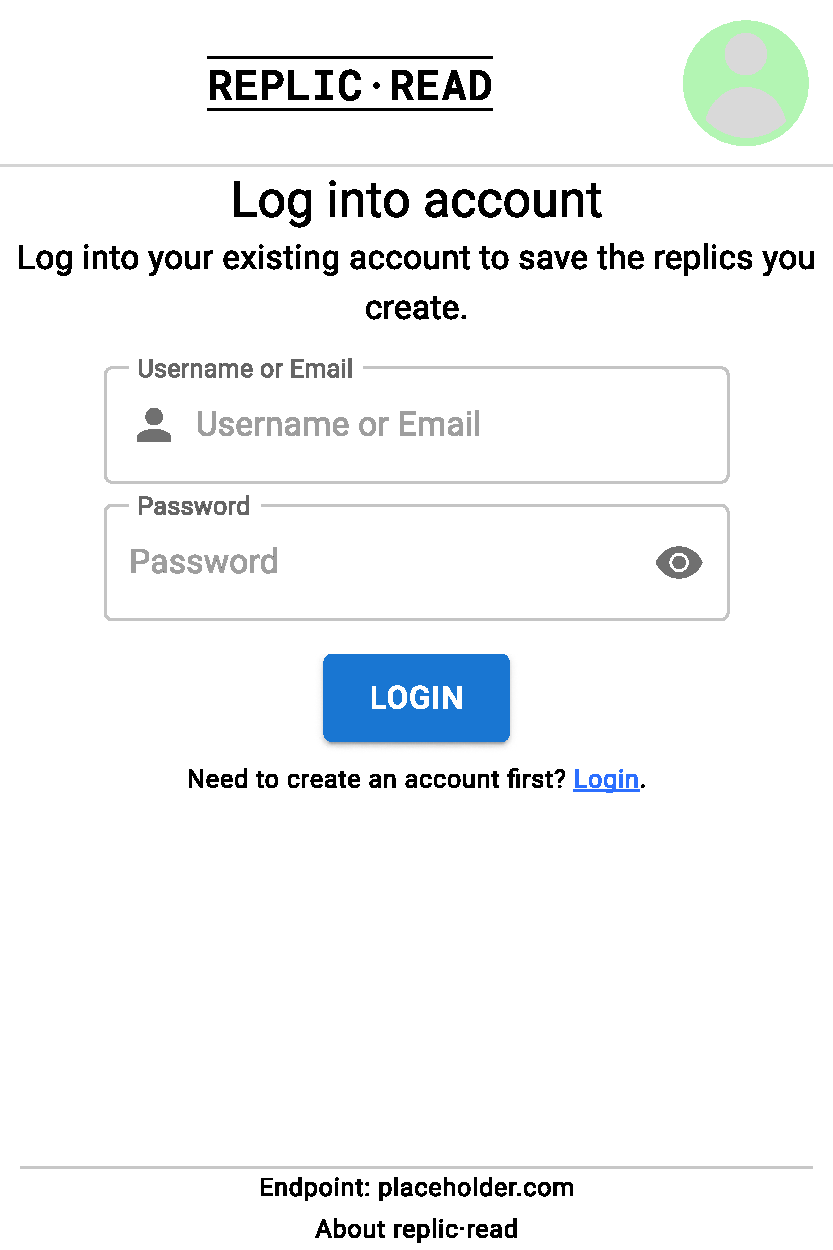
\includegraphics[height=15cm]{ex-login}}

    \caption{Login view}
    \label{fig:ex-login-view}
\end{figure}

\subsubsection{Signup view}
The signup screen (\ref{fig:ex-signup-view}) allows the user to signup (\ref{subsubsec:signup}), or to navigate to the login screen (\ref{fig:ex-login-view}).
\begin{figure}
    \centering
    \fbox{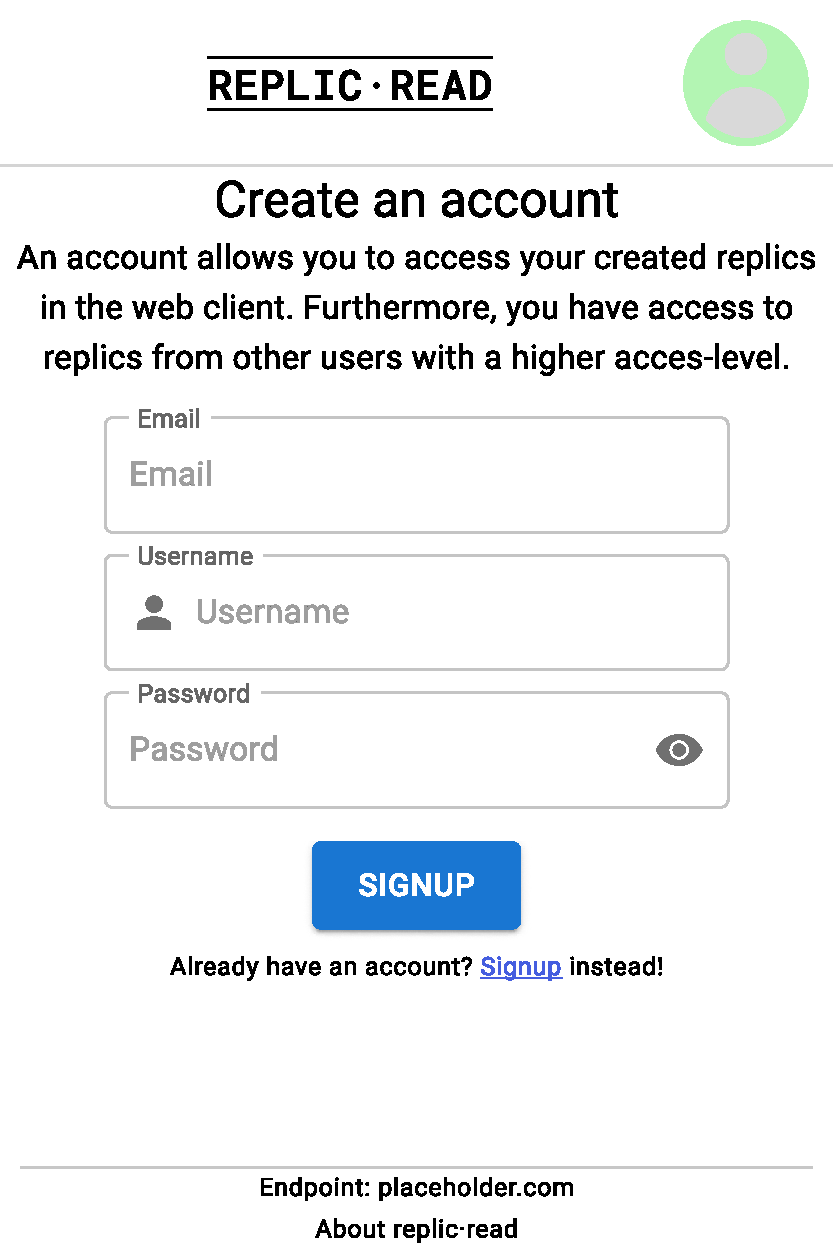
\includegraphics[height=15cm]{ex-signup}}

    \caption{Signup view}
    \label{fig:ex-signup-view}
\end{figure}

\subsubsection{Create replic view}
The create replic view allows a user to create a replic (\ref{subsubsec:create-replic}).
The configuration-panel can be collapsed (\ref{fig:ex-create-replic-view-collapsed}) or expanded (\ref{fig:ex-create-replic-view-expanded}). \newline
After the replic has been created, the user is redirected to (\ref{fig:ex-created-replic-view}).
\begin{figure}
    \centering
    \fbox{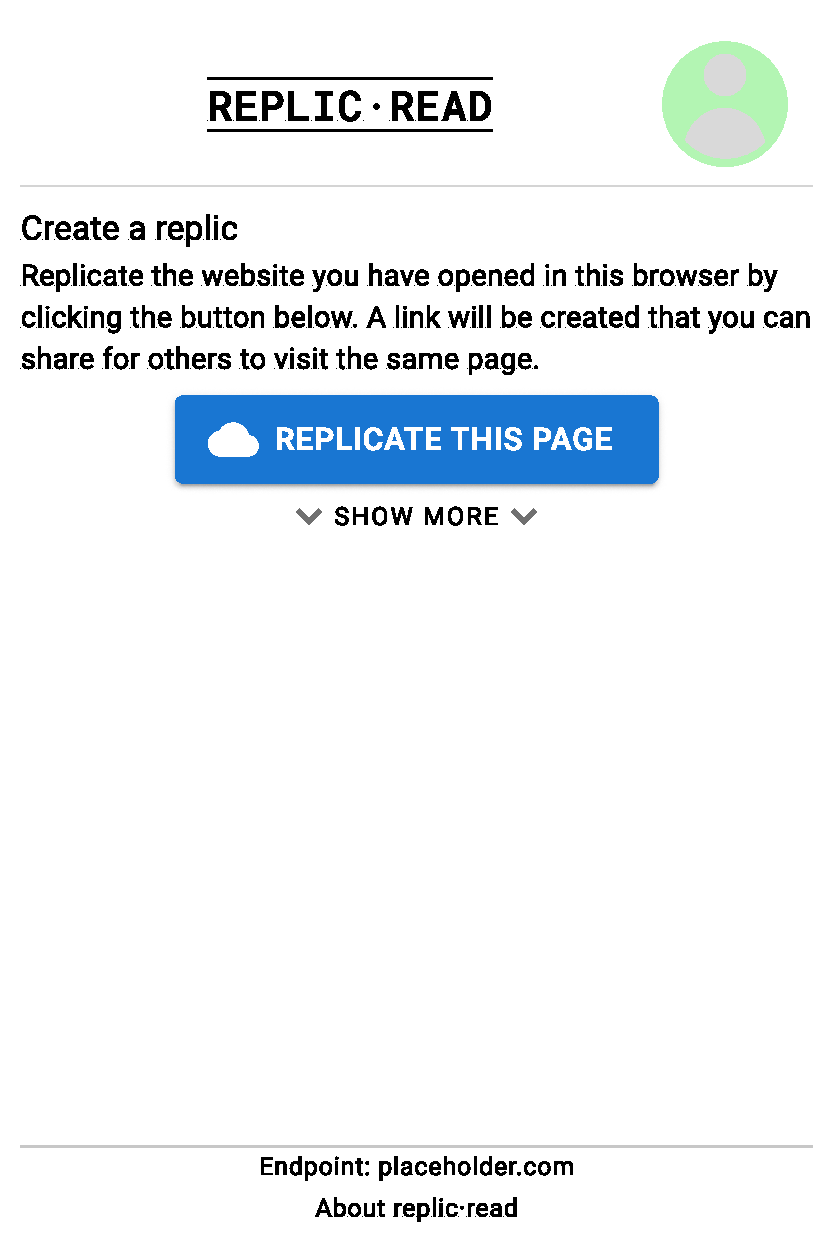
\includegraphics[height=15cm]{ex-create-replic-collapsed}}

    \caption{Create replic view with the configuration menu collapsed}
    \label{fig:ex-create-replic-view-collapsed}
\end{figure}
\begin{figure}
    \centering
    \fbox{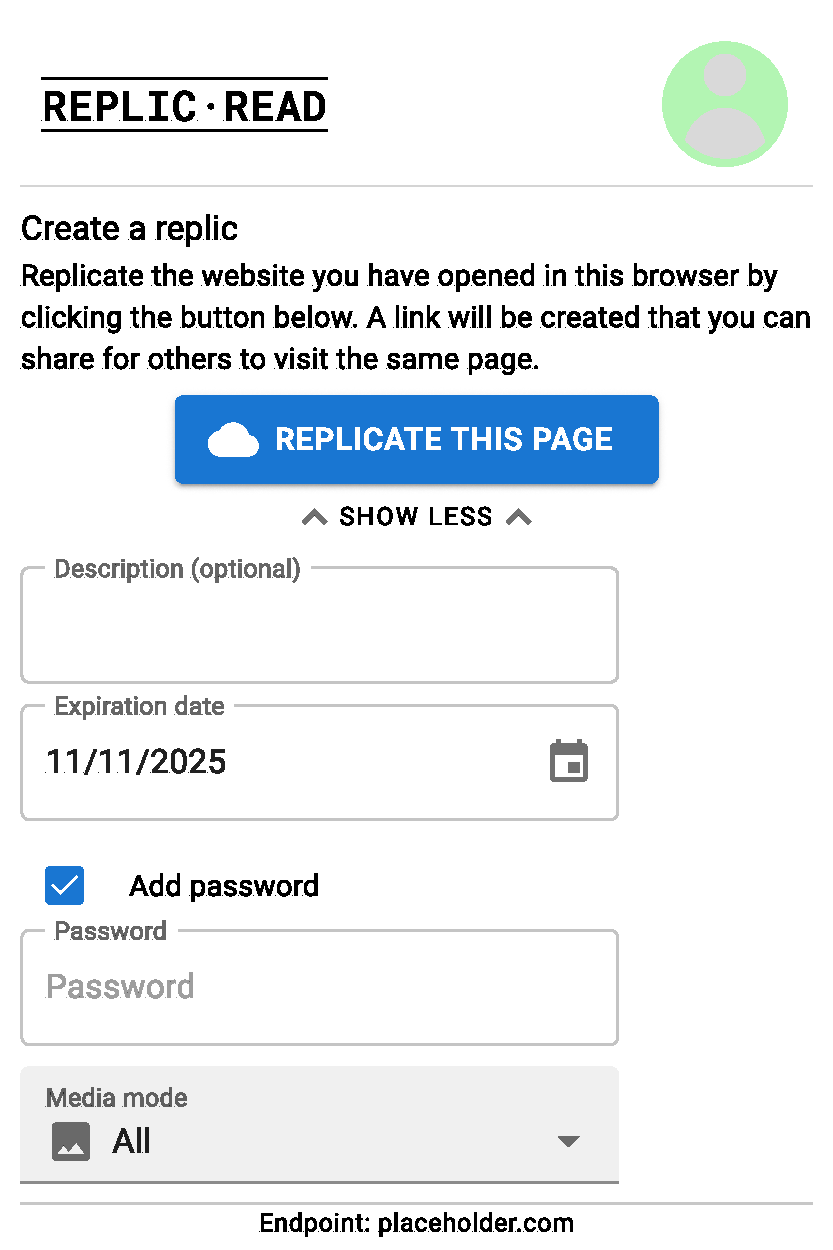
\includegraphics[height=15cm]{ex-create-replic-expanded}}

    \caption{Create replic view with the configuration menu expanded}
    \label{fig:ex-create-replic-view-expanded}
\end{figure}

\subsubsection{Replic created view}
The replic created view shows the user a quick summary of the created replic.
Additionally, the user can copy the target link of the replic that was created (\ref{subsubsec:create-replic}). \newline
A button to create another replic is shown, which will take the user back to the create replic view (\ref{fig:ex-create-replic-view-collapsed})
\begin{figure}
    \centering
    \fbox{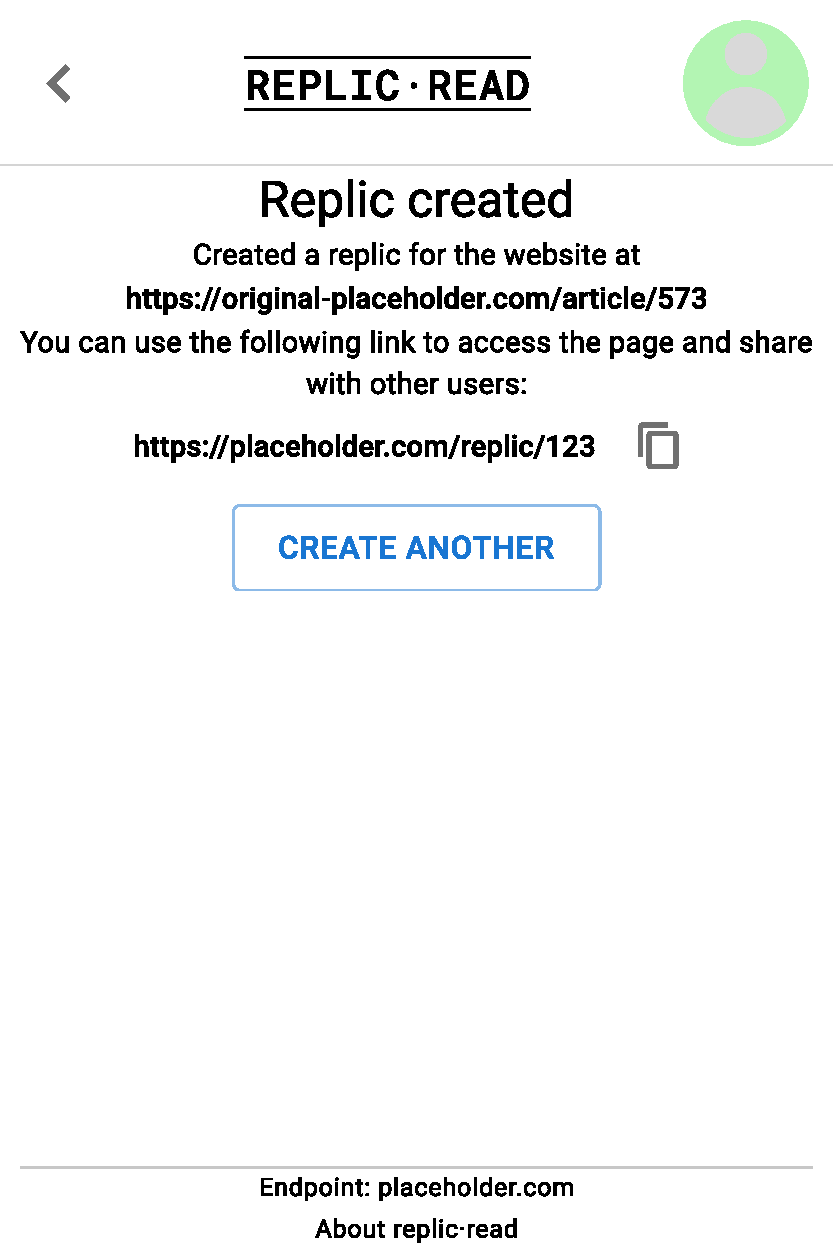
\includegraphics[height=15cm]{ex-replic-created}}

    \caption{Create replic view with the configuration menu expanded}
    \label{fig:ex-created-replic-view}
\end{figure}

\subsubsection{Change endpoint view}
The change endpoint view allows the user to set/change the endpoint the client connects to (\ref{subsubsec:change-server-endpoint}).
This view is navigated to by clicking the endpoint info in the footer. \newline
Depending on whether the user is logged in or -out, and whether an endpoint has already been set, one of~\ref{fig:ex-change-endpoint-view-none-logged-out},~\ref{fig:ex-change-endpoint-view-present-logged-out},~\ref{fig:ex-change-endpoint-view-present-logged-in} is shown.
\begin{figure}
    \centering
    \fbox{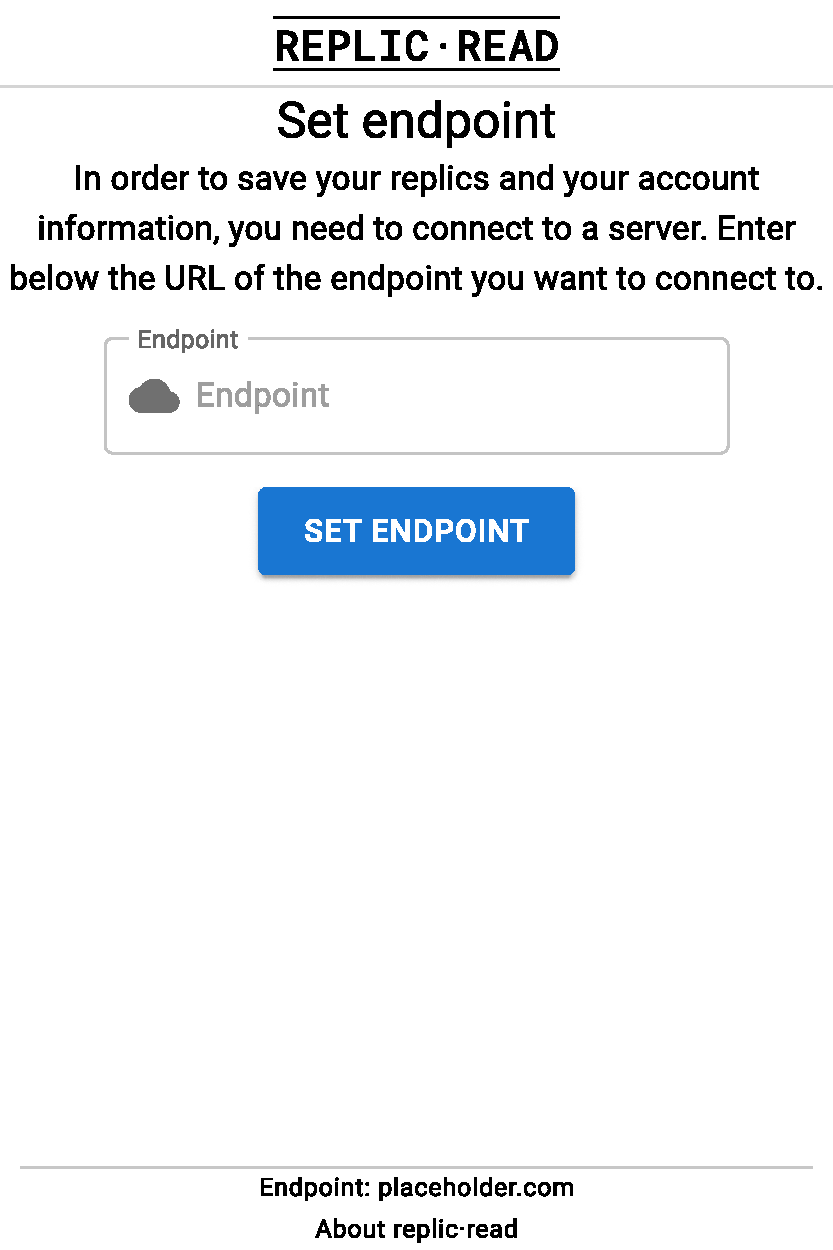
\includegraphics[height=15cm]{ex-change-endpoint-none-logged-out}}

    \caption{Change endpoint screen when the endpoint has to be initially set, and the user is logged out.}
    \label{fig:ex-change-endpoint-view-none-logged-out}
\end{figure}
\begin{figure}
    \centering
    \fbox{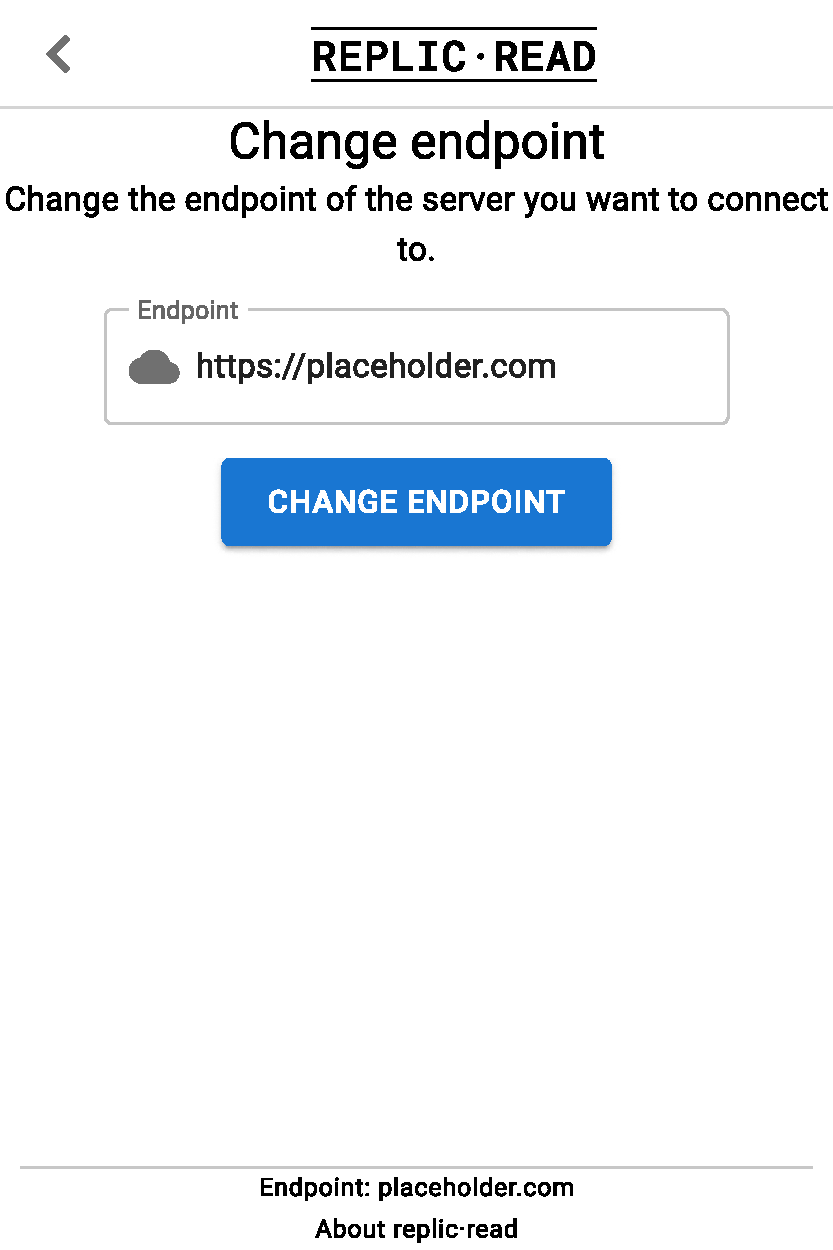
\includegraphics[height=15cm]{ex-change-endpoint-present-logged-out}}

    \caption{Change endpoint screen when the endpoint has already been set, and the user is logged out.}
    \label{fig:ex-change-endpoint-view-present-logged-out}
\end{figure}
\begin{figure}
    \centering
    \fbox{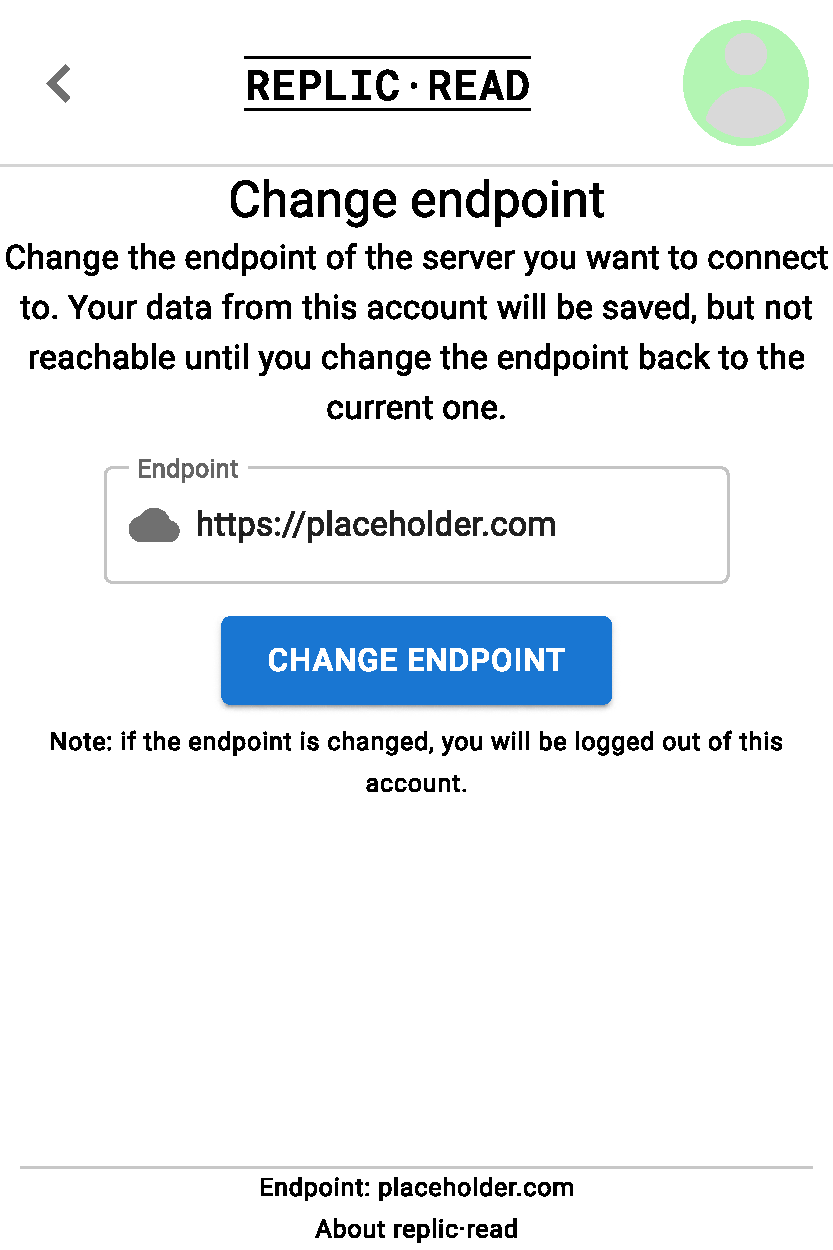
\includegraphics[height=15cm]{ex-change-endpoint-present-logged-in}}

    \caption{Change endpoint screen when the endpoint has already been set, and the user is logged in.}
    \label{fig:ex-change-endpoint-view-present-logged-in}
\end{figure}

\subsubsection{Account menu}
The account menu (\ref{fig:ex-account-menu-view}) gives context actions for the user related to the account, namely to logout (\ref{subsubsec:logout}).
Clicking on the account icon in the top right-hand corner navigates here.

\begin{figure}
    \centering
    \fbox{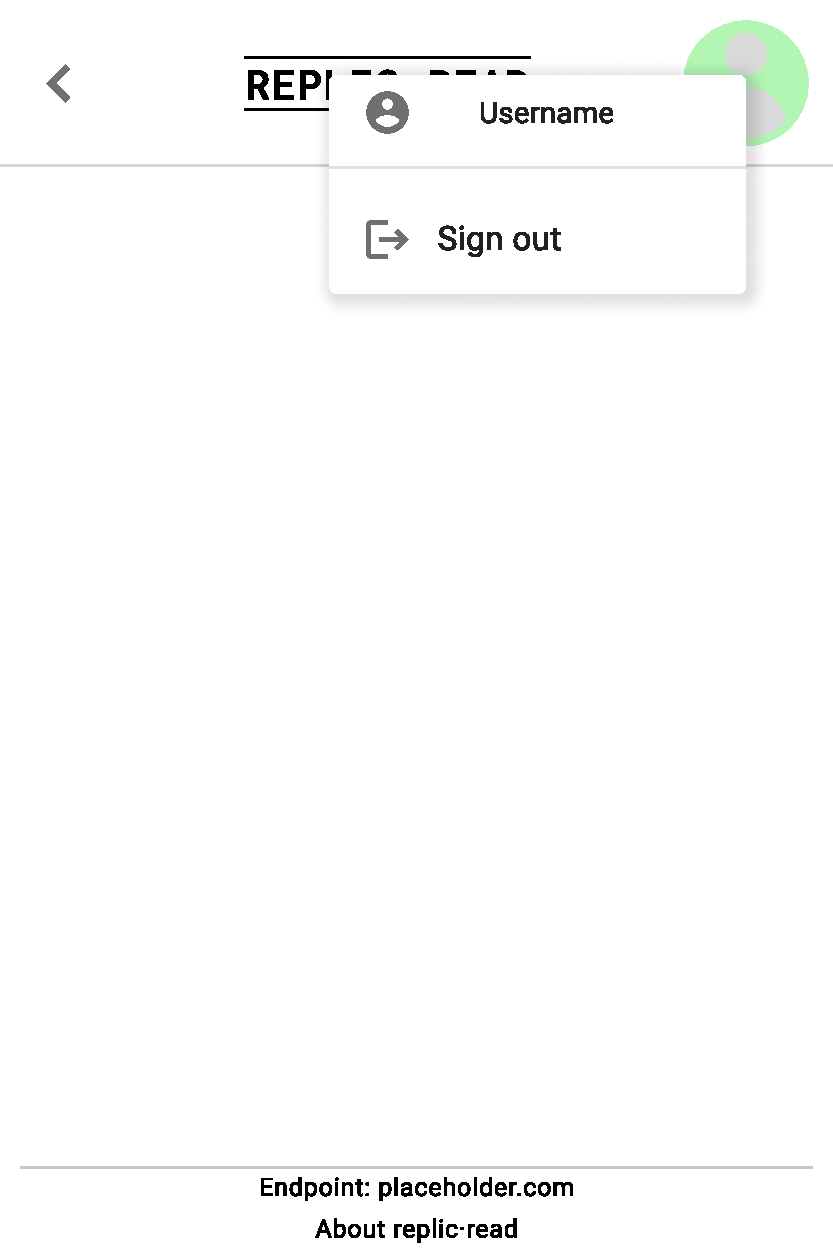
\includegraphics[height=15cm]{ex-account-menu}}

    \caption{Account menu.}
    \label{fig:ex-account-menu-view}
\end{figure}

\subsubsection{Unverified account view}
The account-not-verified view (\ref{fig:ex-account-not-verified-view}) shows an informative text to notify the user that the email has not yet been verified.
The user also has the option to request a new link.

\begin{figure}
    \centering
    \fbox{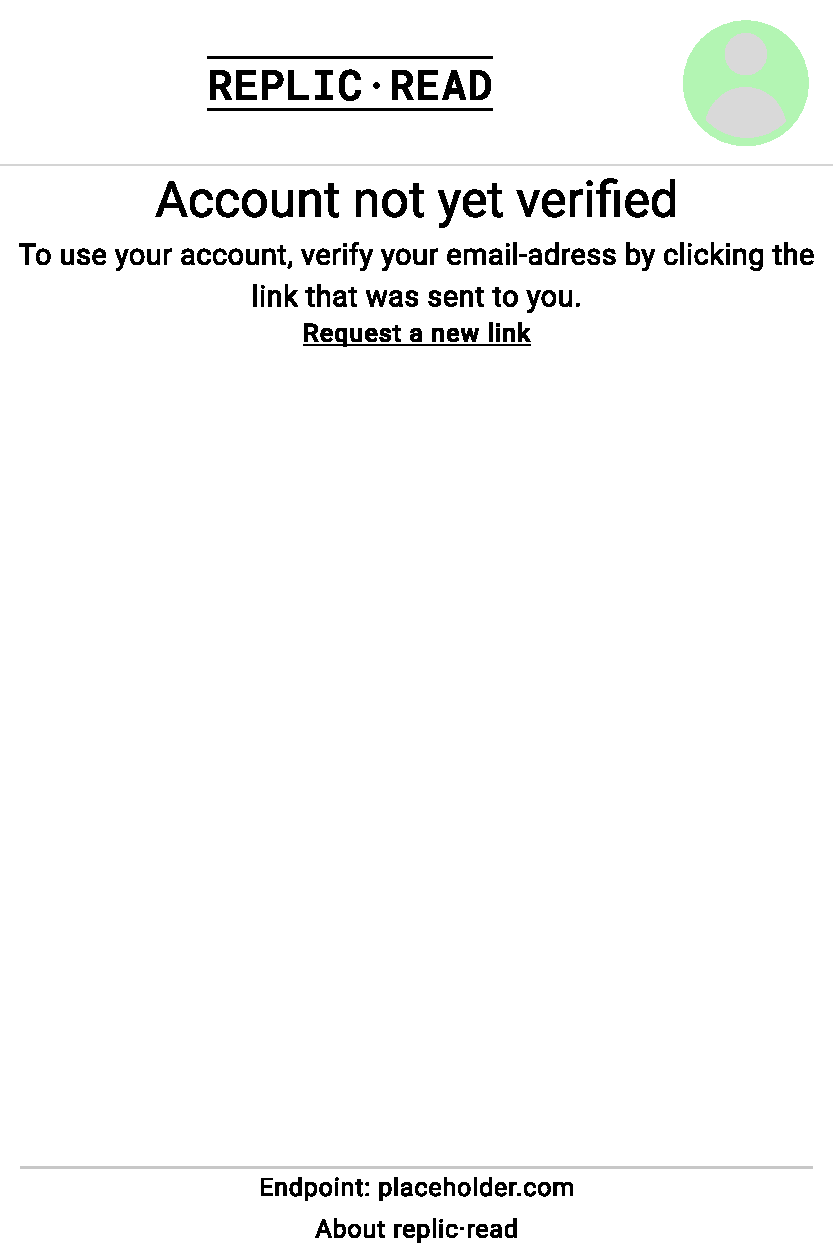
\includegraphics[height=15cm]{ex-account-not-verified}}

    \caption{Account not yet verified.}
    \label{fig:ex-account-not-verified-view}
\end{figure}

\subsection{Web-Client}\label{subsec:web-client}
The user-interface for the web-client will run in any browser thatis supported.
Mobile-adaptive layouts are not supported.
The following graphics depict the screens on a default \SI{400}{px} by \SI{600}{px} desktop environment.
Due to size constraints, the mockups are presented in small display.
The full-size graphics can be found in the appendix.

\subsubsection{Login View}
The login screen (\ref{fig:web-login-view}) allows the user to login (\ref{subsubsec:login}), or to navigate to the signup view (\ref{fig:web-signup-view}) if an account should be created.
\begin{figure}
    \centering
    \fbox{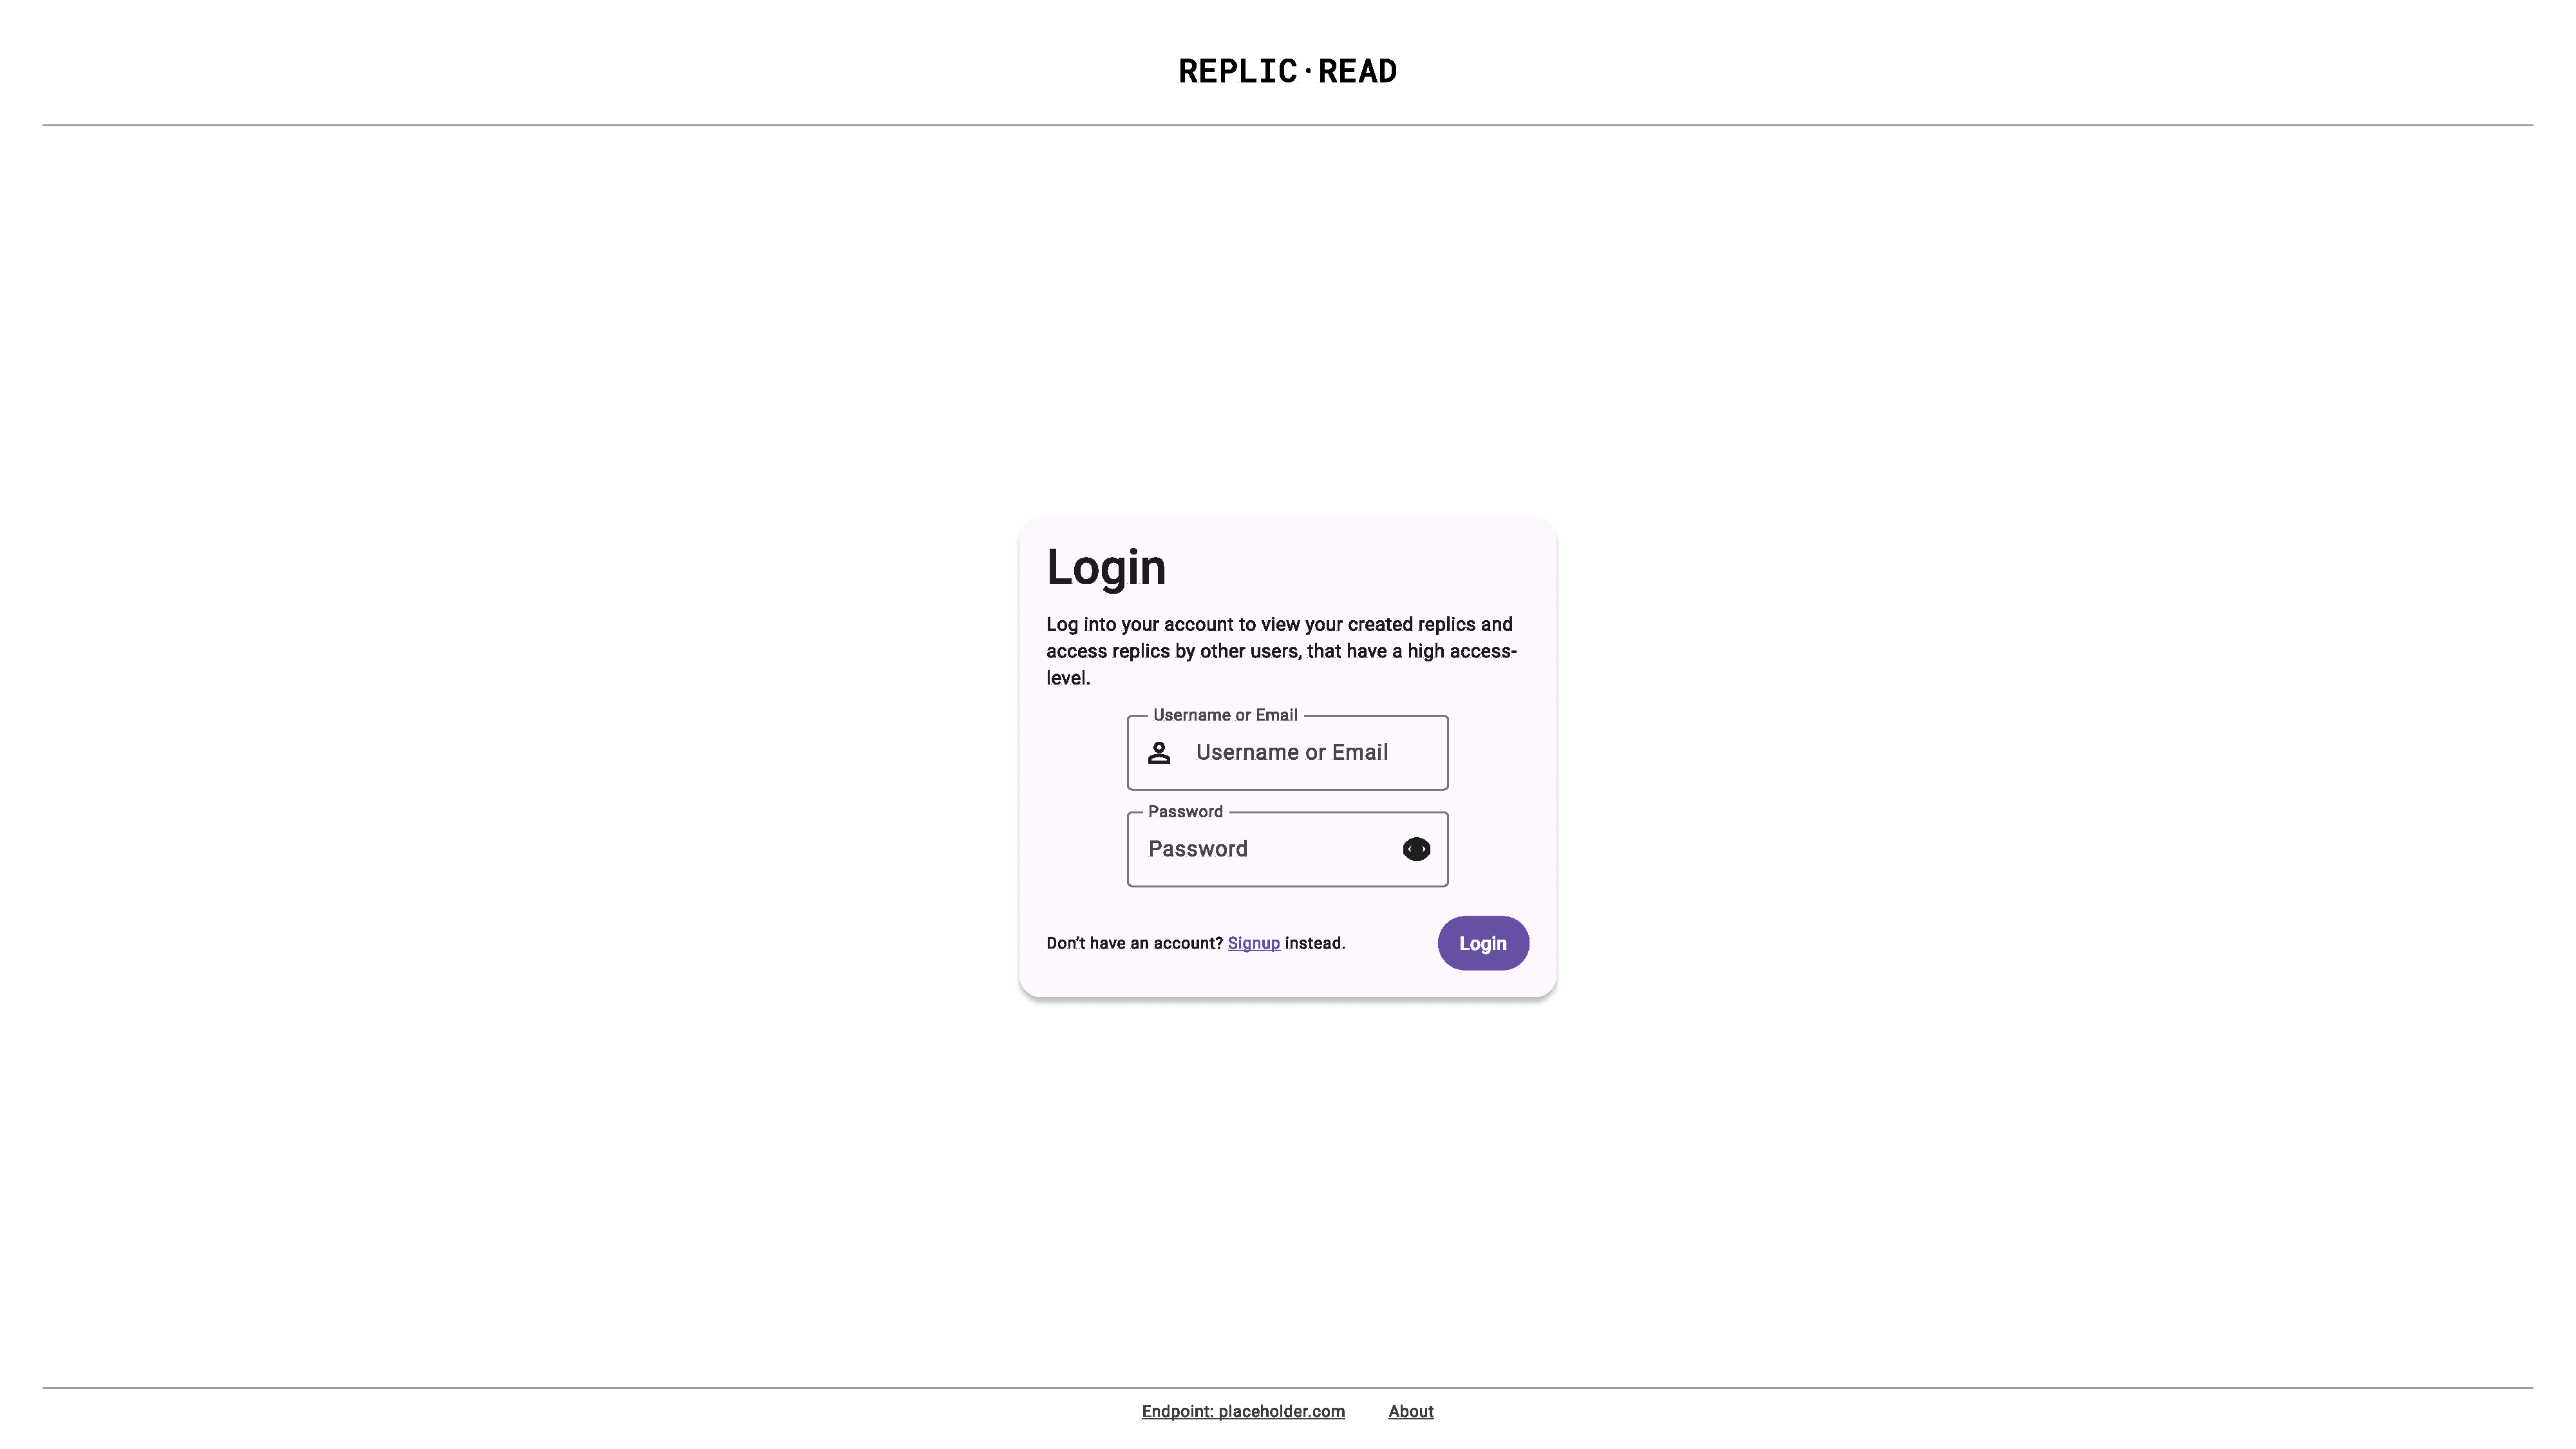
\includegraphics[width=12cm]{web-login}}

    \caption{Login view}
    \label{fig:web-login-view}
\end{figure}

\subsubsection{Signup View}
The signup screen (\ref{fig:web-signup-view}) allows the user to signup (\ref{subsubsec:signup}), or to navigate to the signup view (\ref{fig:web-login-view}) if an account already exists.
\begin{figure}
    \centering
    \fbox{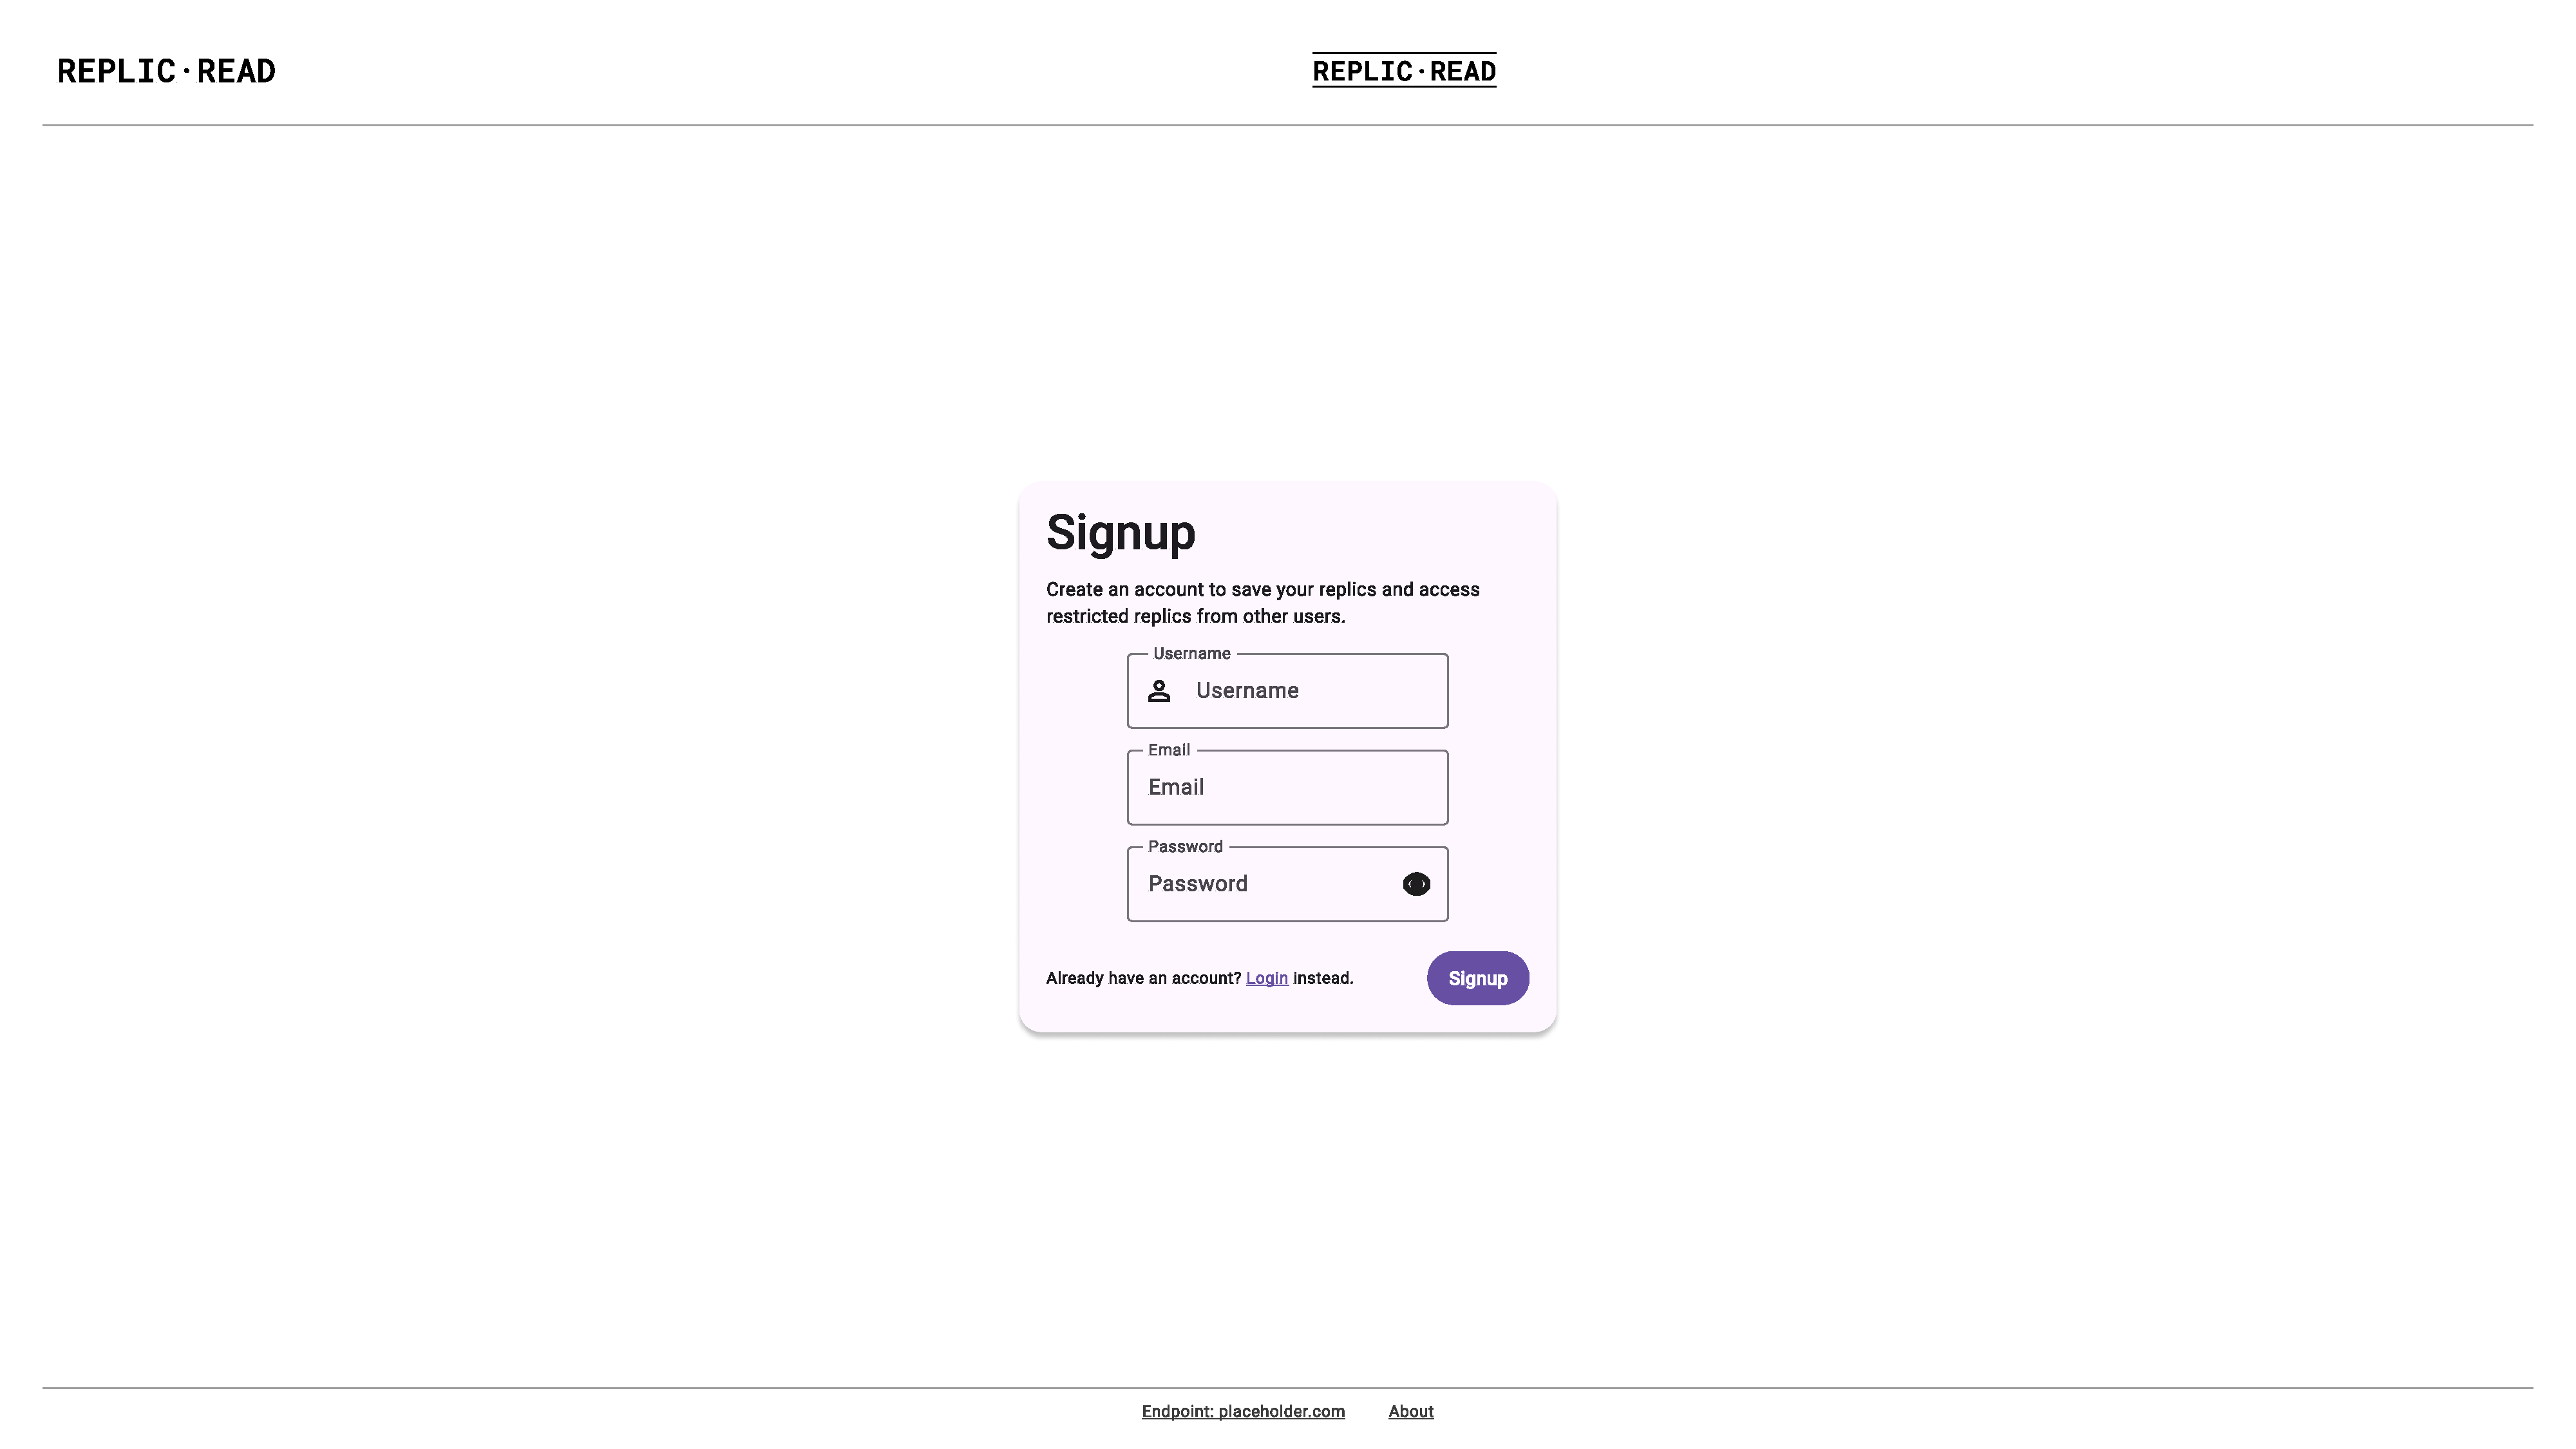
\includegraphics[width=12cm]{web-signup}}

    \caption{Signup view}
    \label{fig:web-signup-view}
\end{figure}

\subsubsection{Account View}
The account screen (\ref{fig:web-account-view}) shows basic information about the current account to the user.
Additionally, the user can change the username (\ref{subsubsec:change-username}), email (\ref{subsubsec:change-email}) and account color (\ref{subsubsec:change-color}).
A requested email-verification email can be cancelled.
\begin{figure}
    \centering
    \fbox{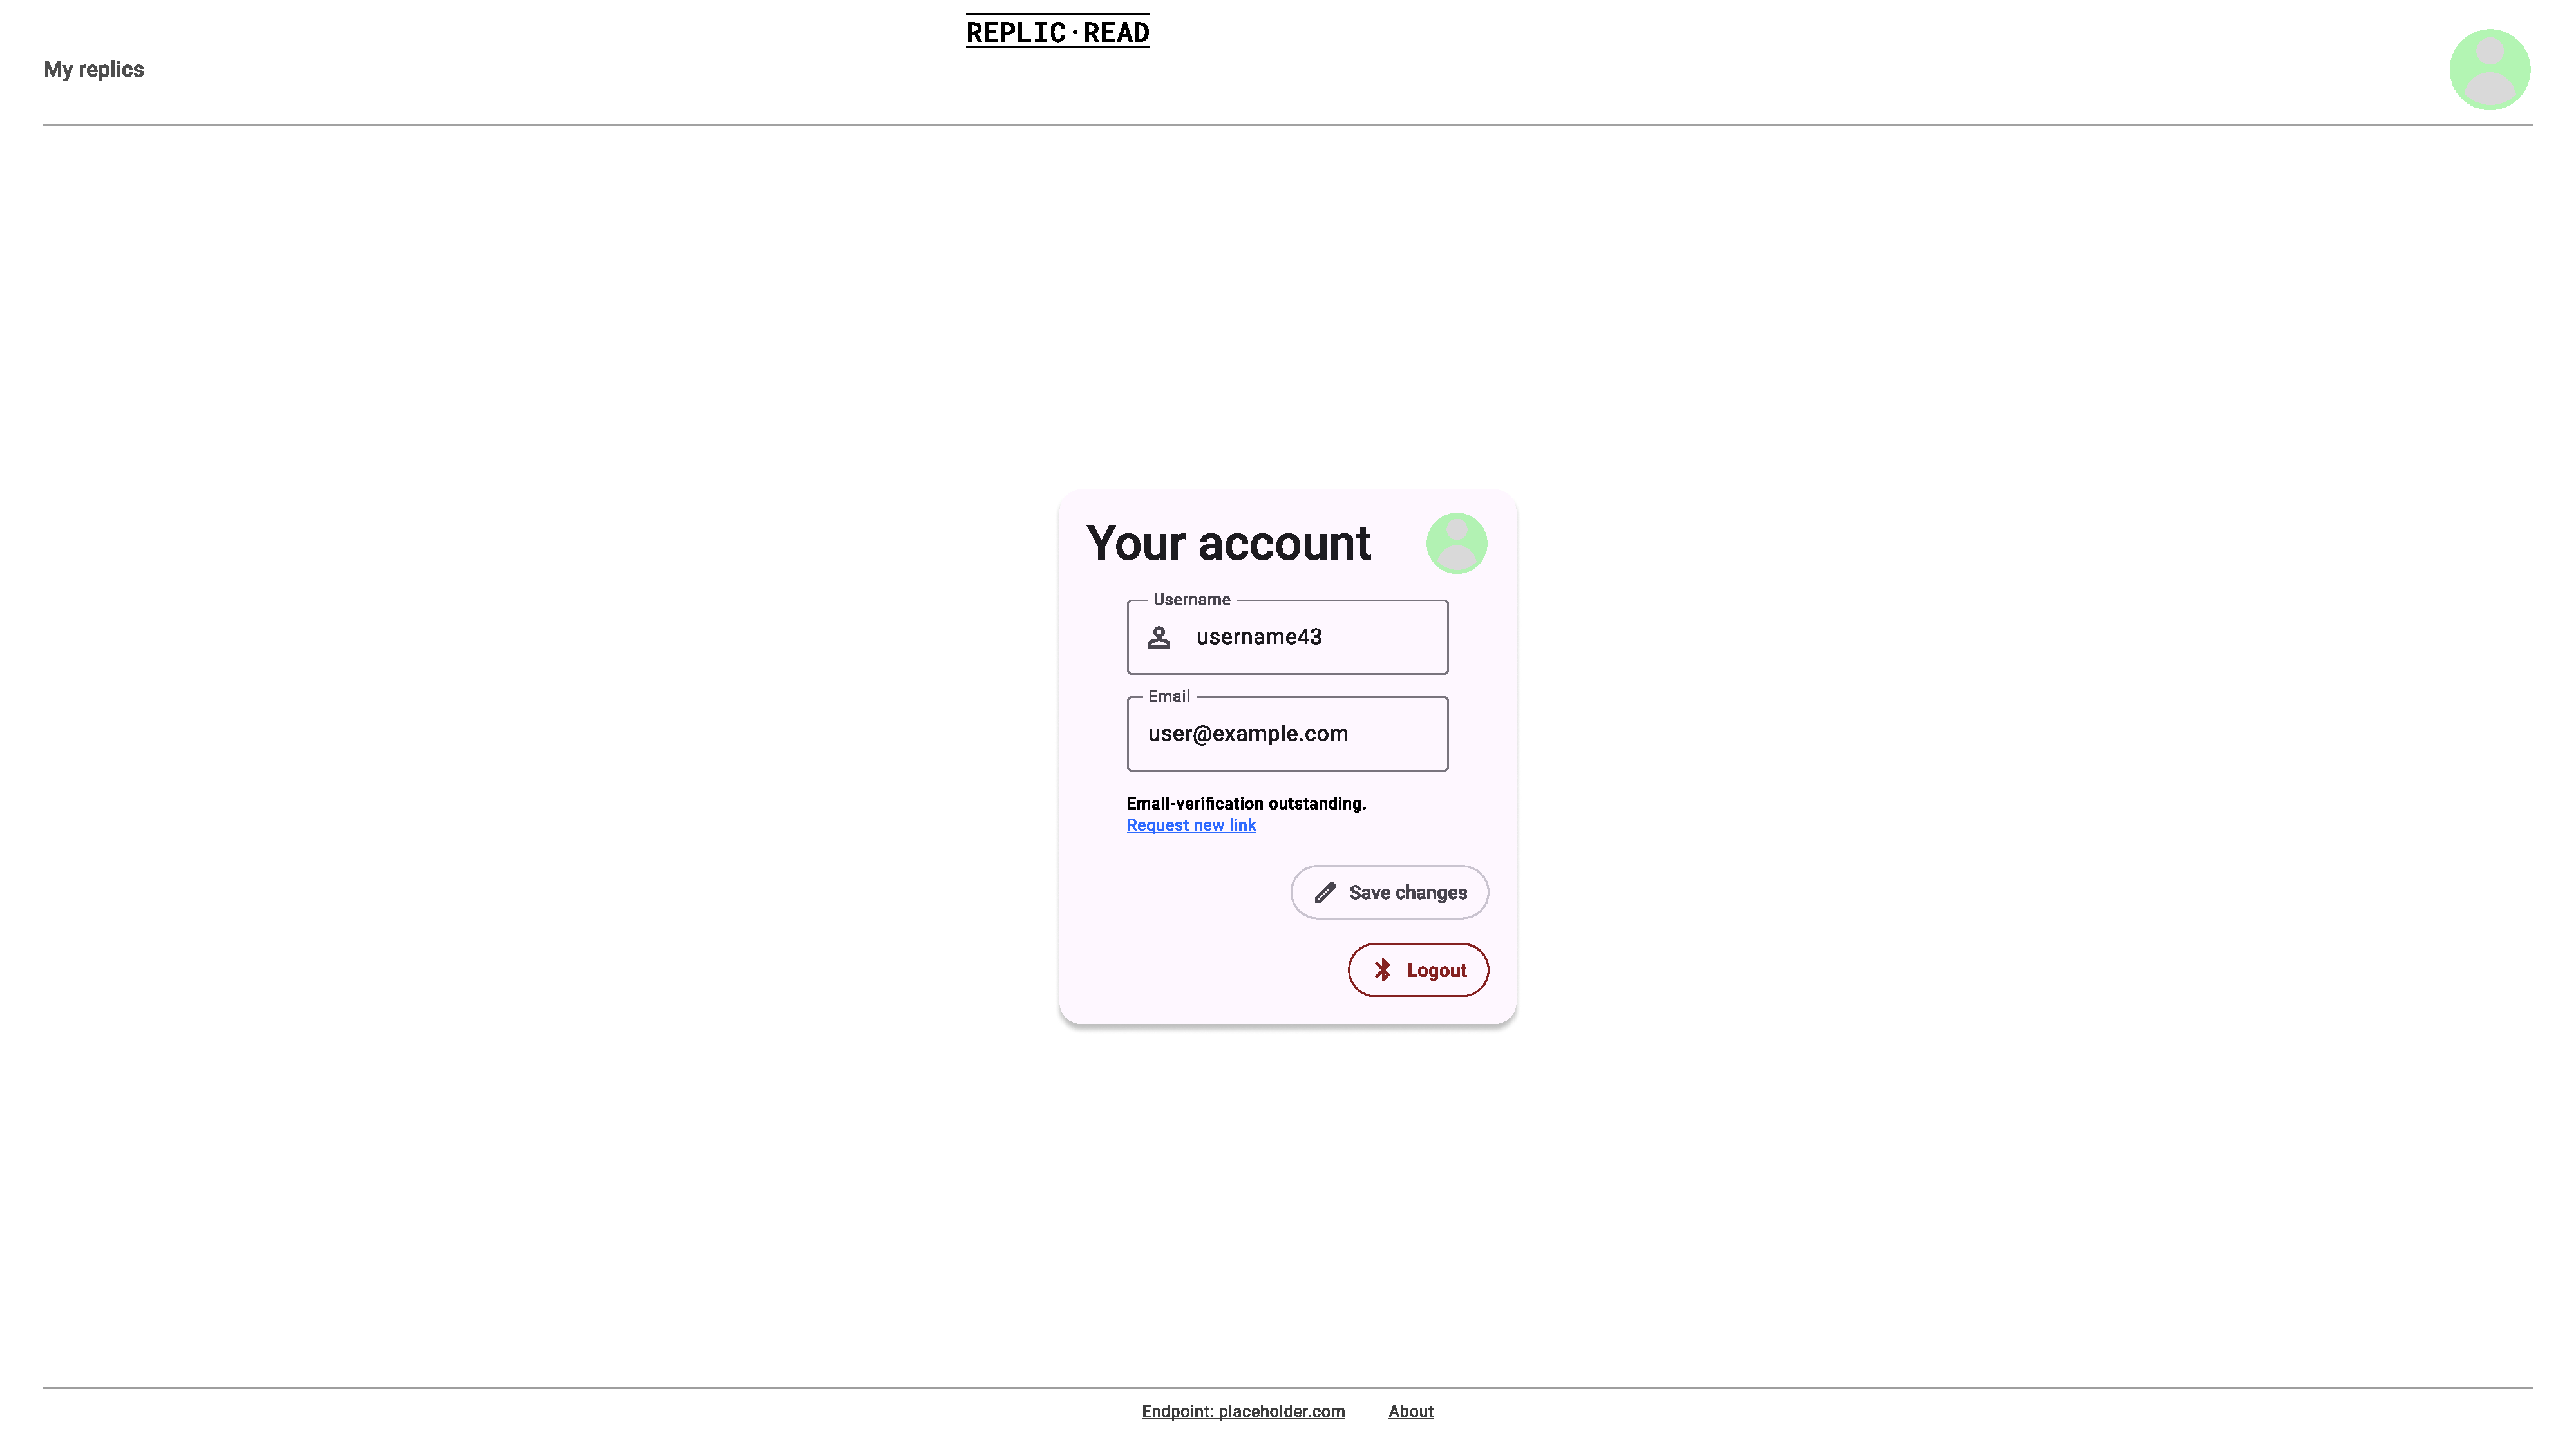
\includegraphics[width=12cm]{web-account}}

    \caption{Account view}
    \label{fig:web-account-view}
\end{figure}

\subsubsection{Admin config View}
The admin config view (\ref{fig:web-config-view}) allows the admin account to perform all the config changes that are available.
Additionally, there is a panel for an admin to create a user (\ref{subsubsec:create-user}).
\begin{figure}
    \centering
    \fbox{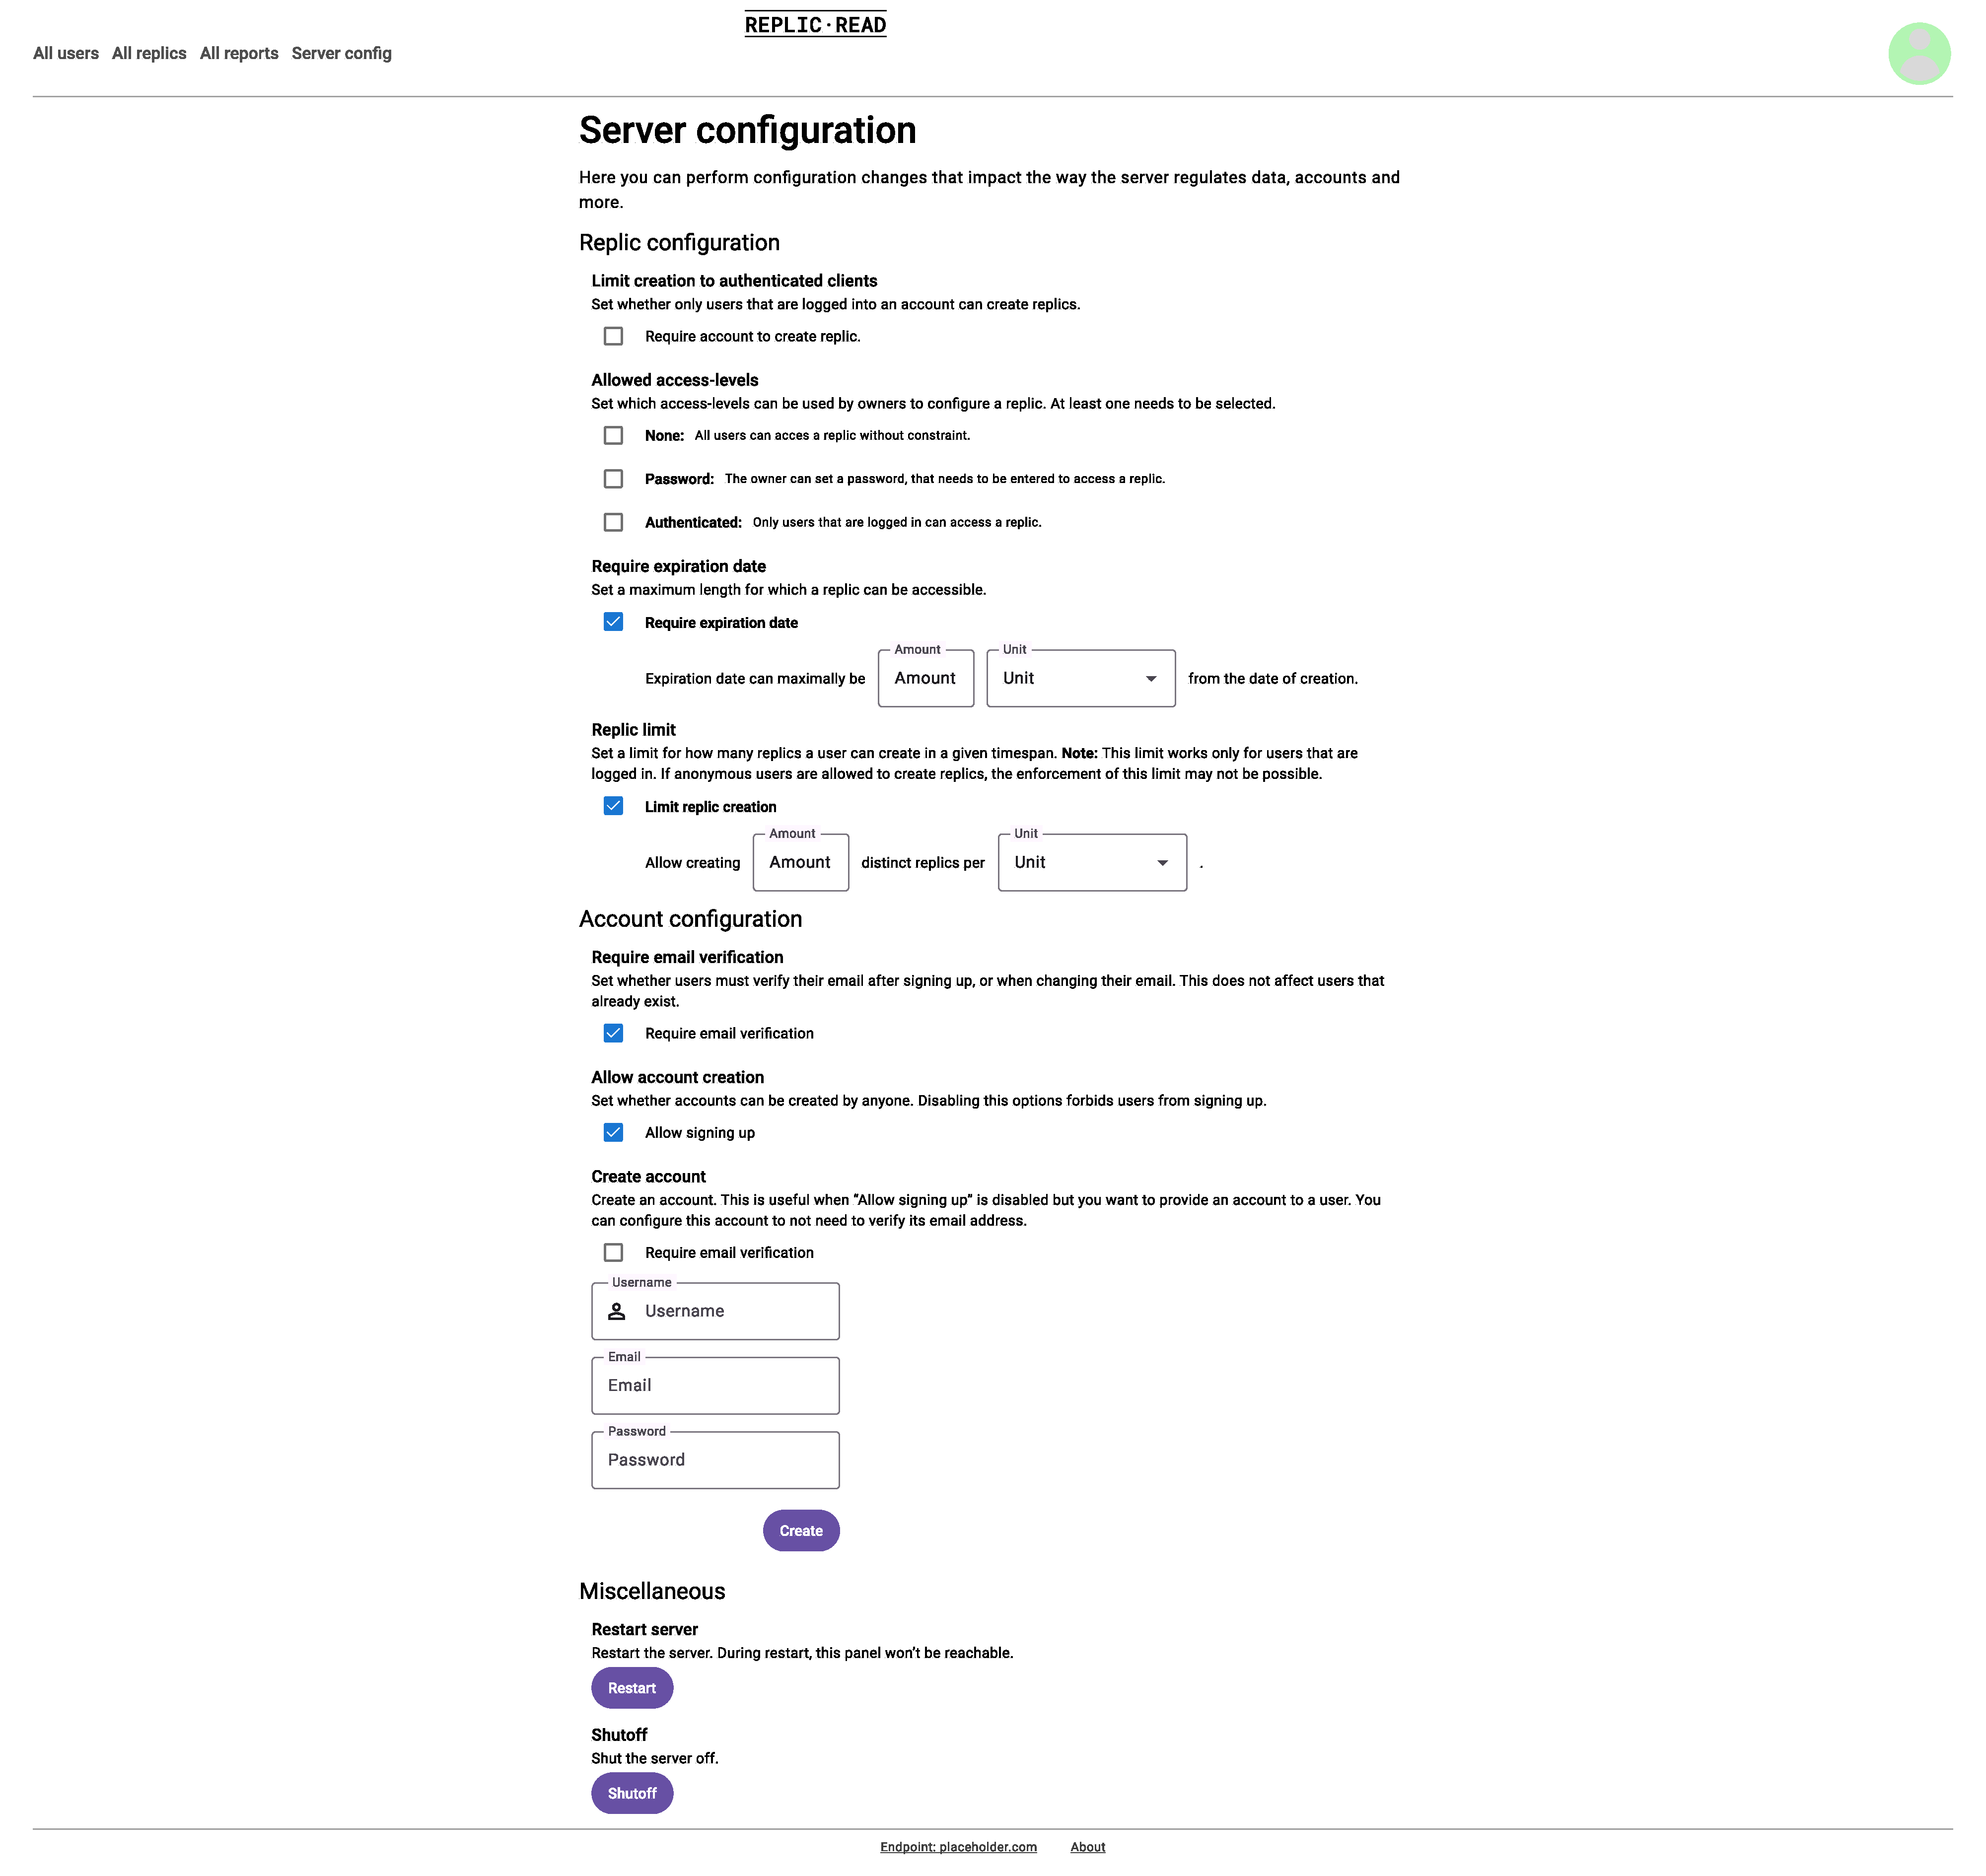
\includegraphics[width=12cm]{web-config}}

    \caption{Admin config view}
    \label{fig:web-config-view}
\end{figure}

\subsubsection{User replics view}
The user replics view gives a user an overview of the replics created by the account.
Each replic is represented by an item in a list that shows the original link, description, size, expiration date and state.
Each item has context actions that allow the user to deactivate (\ref{subsubsec:deactivate-replic}) or reactivate (\ref{subsubsec:reactivate-replic}) the replic.
The replics can be searched using a search bar, and filtered/sorted by using the sorting config that can be expanded (\ref{fig:web-user-replics-config-view}) or collapsed (\ref{fig:web-user-replics-noconfig-view}).
\begin{figure}
    \centering
    \fbox{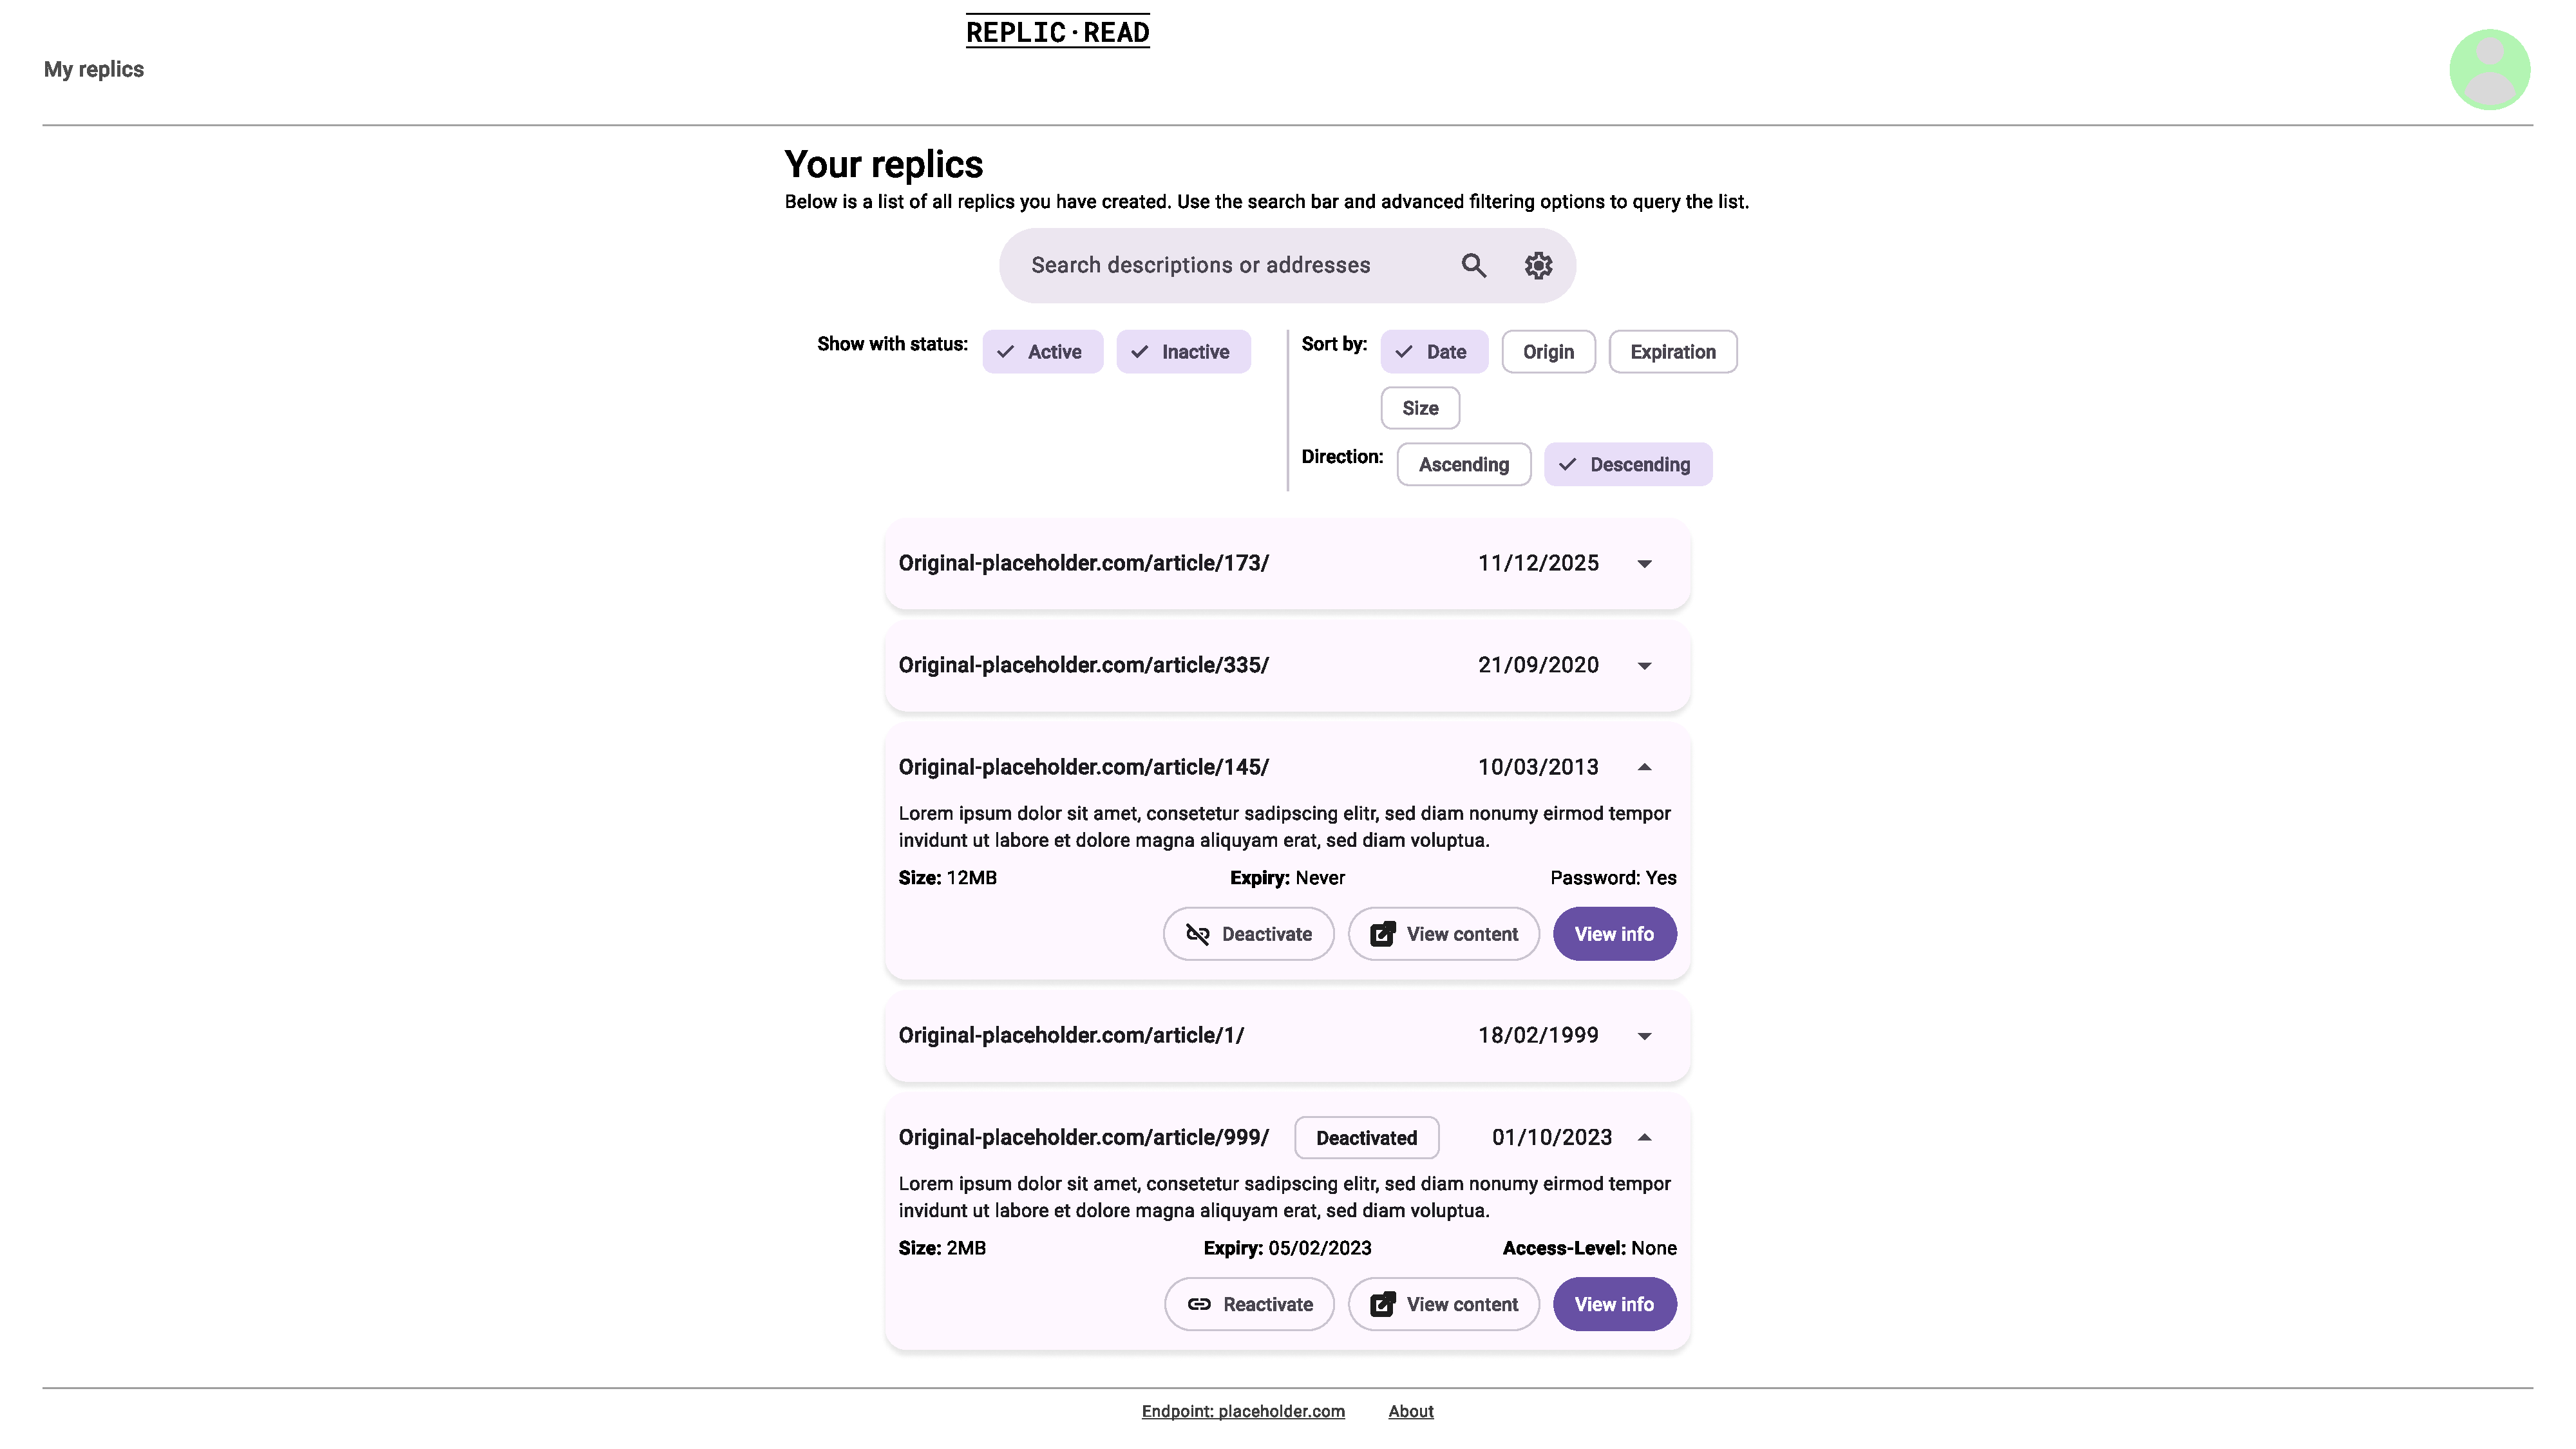
\includegraphics[width=12cm]{web-user-replics-config}}

    \caption{User replics view with search config visible}
    \label{fig:web-user-replics-config-view}
\end{figure}
\begin{figure}
    \centering
    \fbox{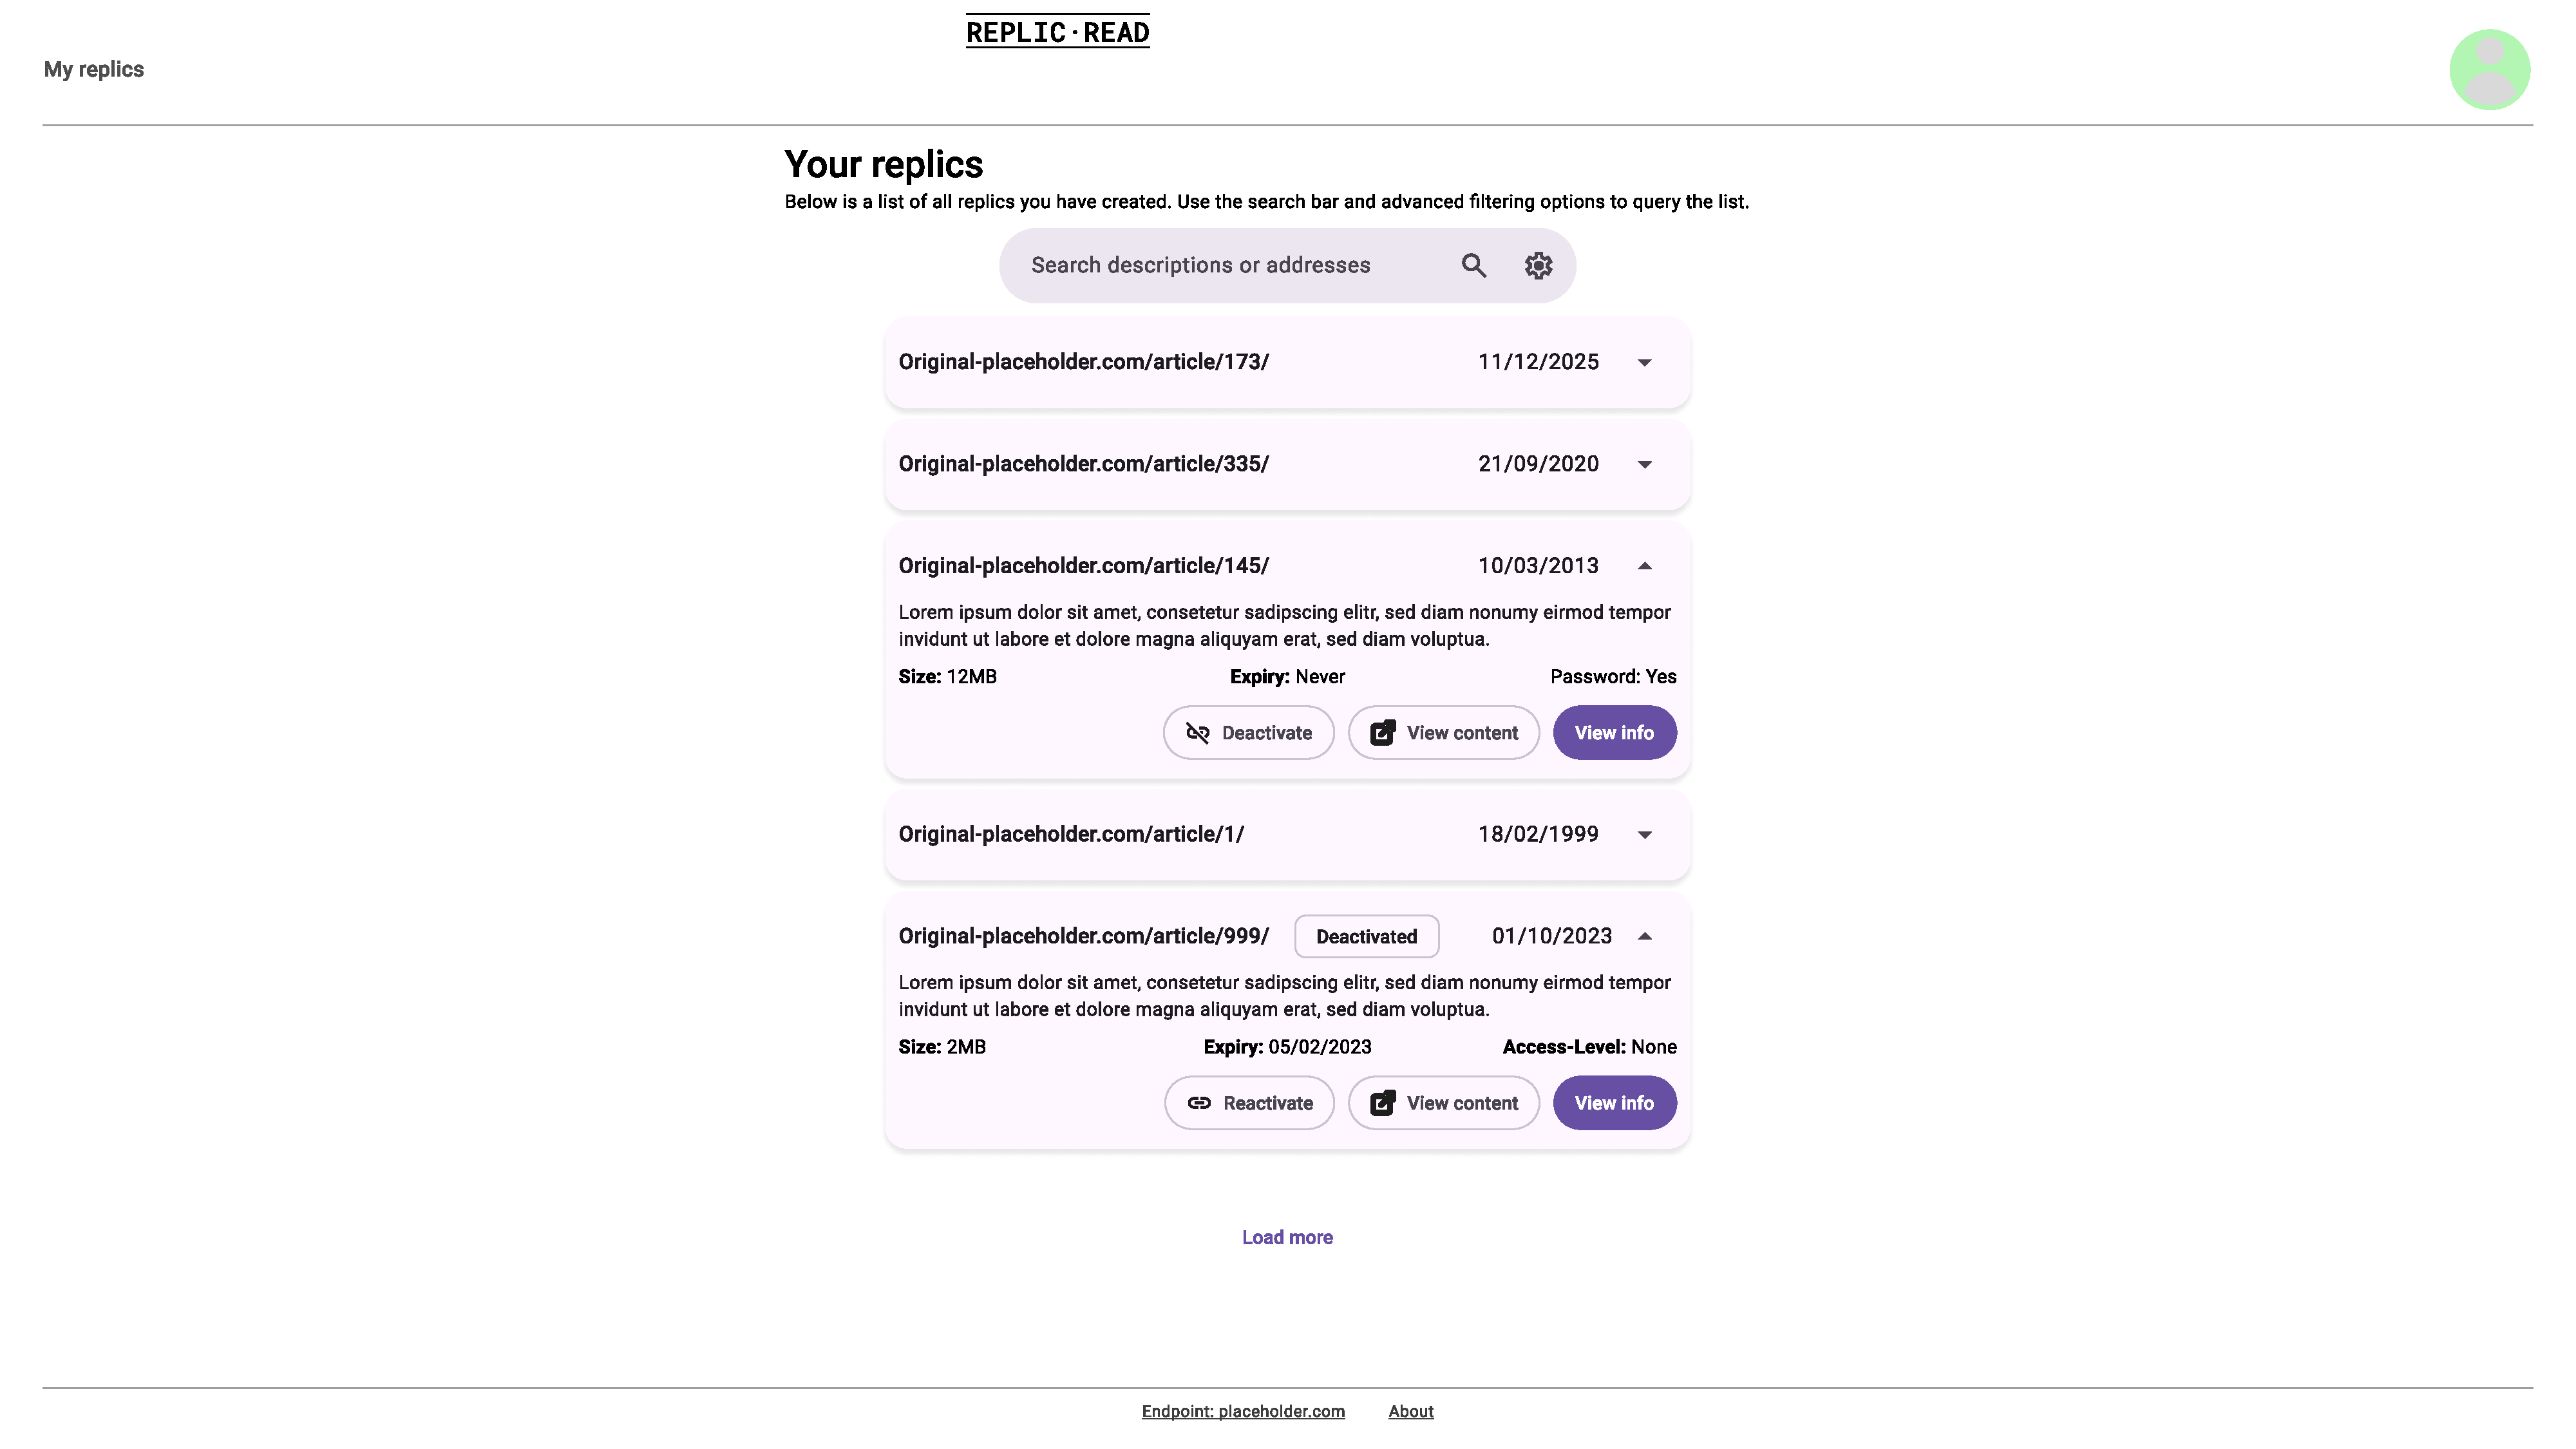
\includegraphics[width=12cm]{web-user-replics-noconfig}}

    \caption{User replics view}
    \label{fig:web-user-replics-noconfig-view}
\end{figure}

\subsubsection{Admin replics view}
The admin replics view allows the admin to view all replics created on the server.
Each replic is represented by an item in a list that shows the original link, description, size, expiration date and state.
Each item has config actions that allows the admin to remove (\ref{subsubsec:remove-replic}) or restore a replic.
The replics can be searched using a search bar, and filtered/sorted by using the sorting config that can be expanded (\ref{fig:web-admin-replics-config-view}) or collapsed (\ref{fig:web-admin-replics-noconfig-view}).
A dropdown to filter the replics by authoring user is also available.
\begin{figure}
    \centering
    \fbox{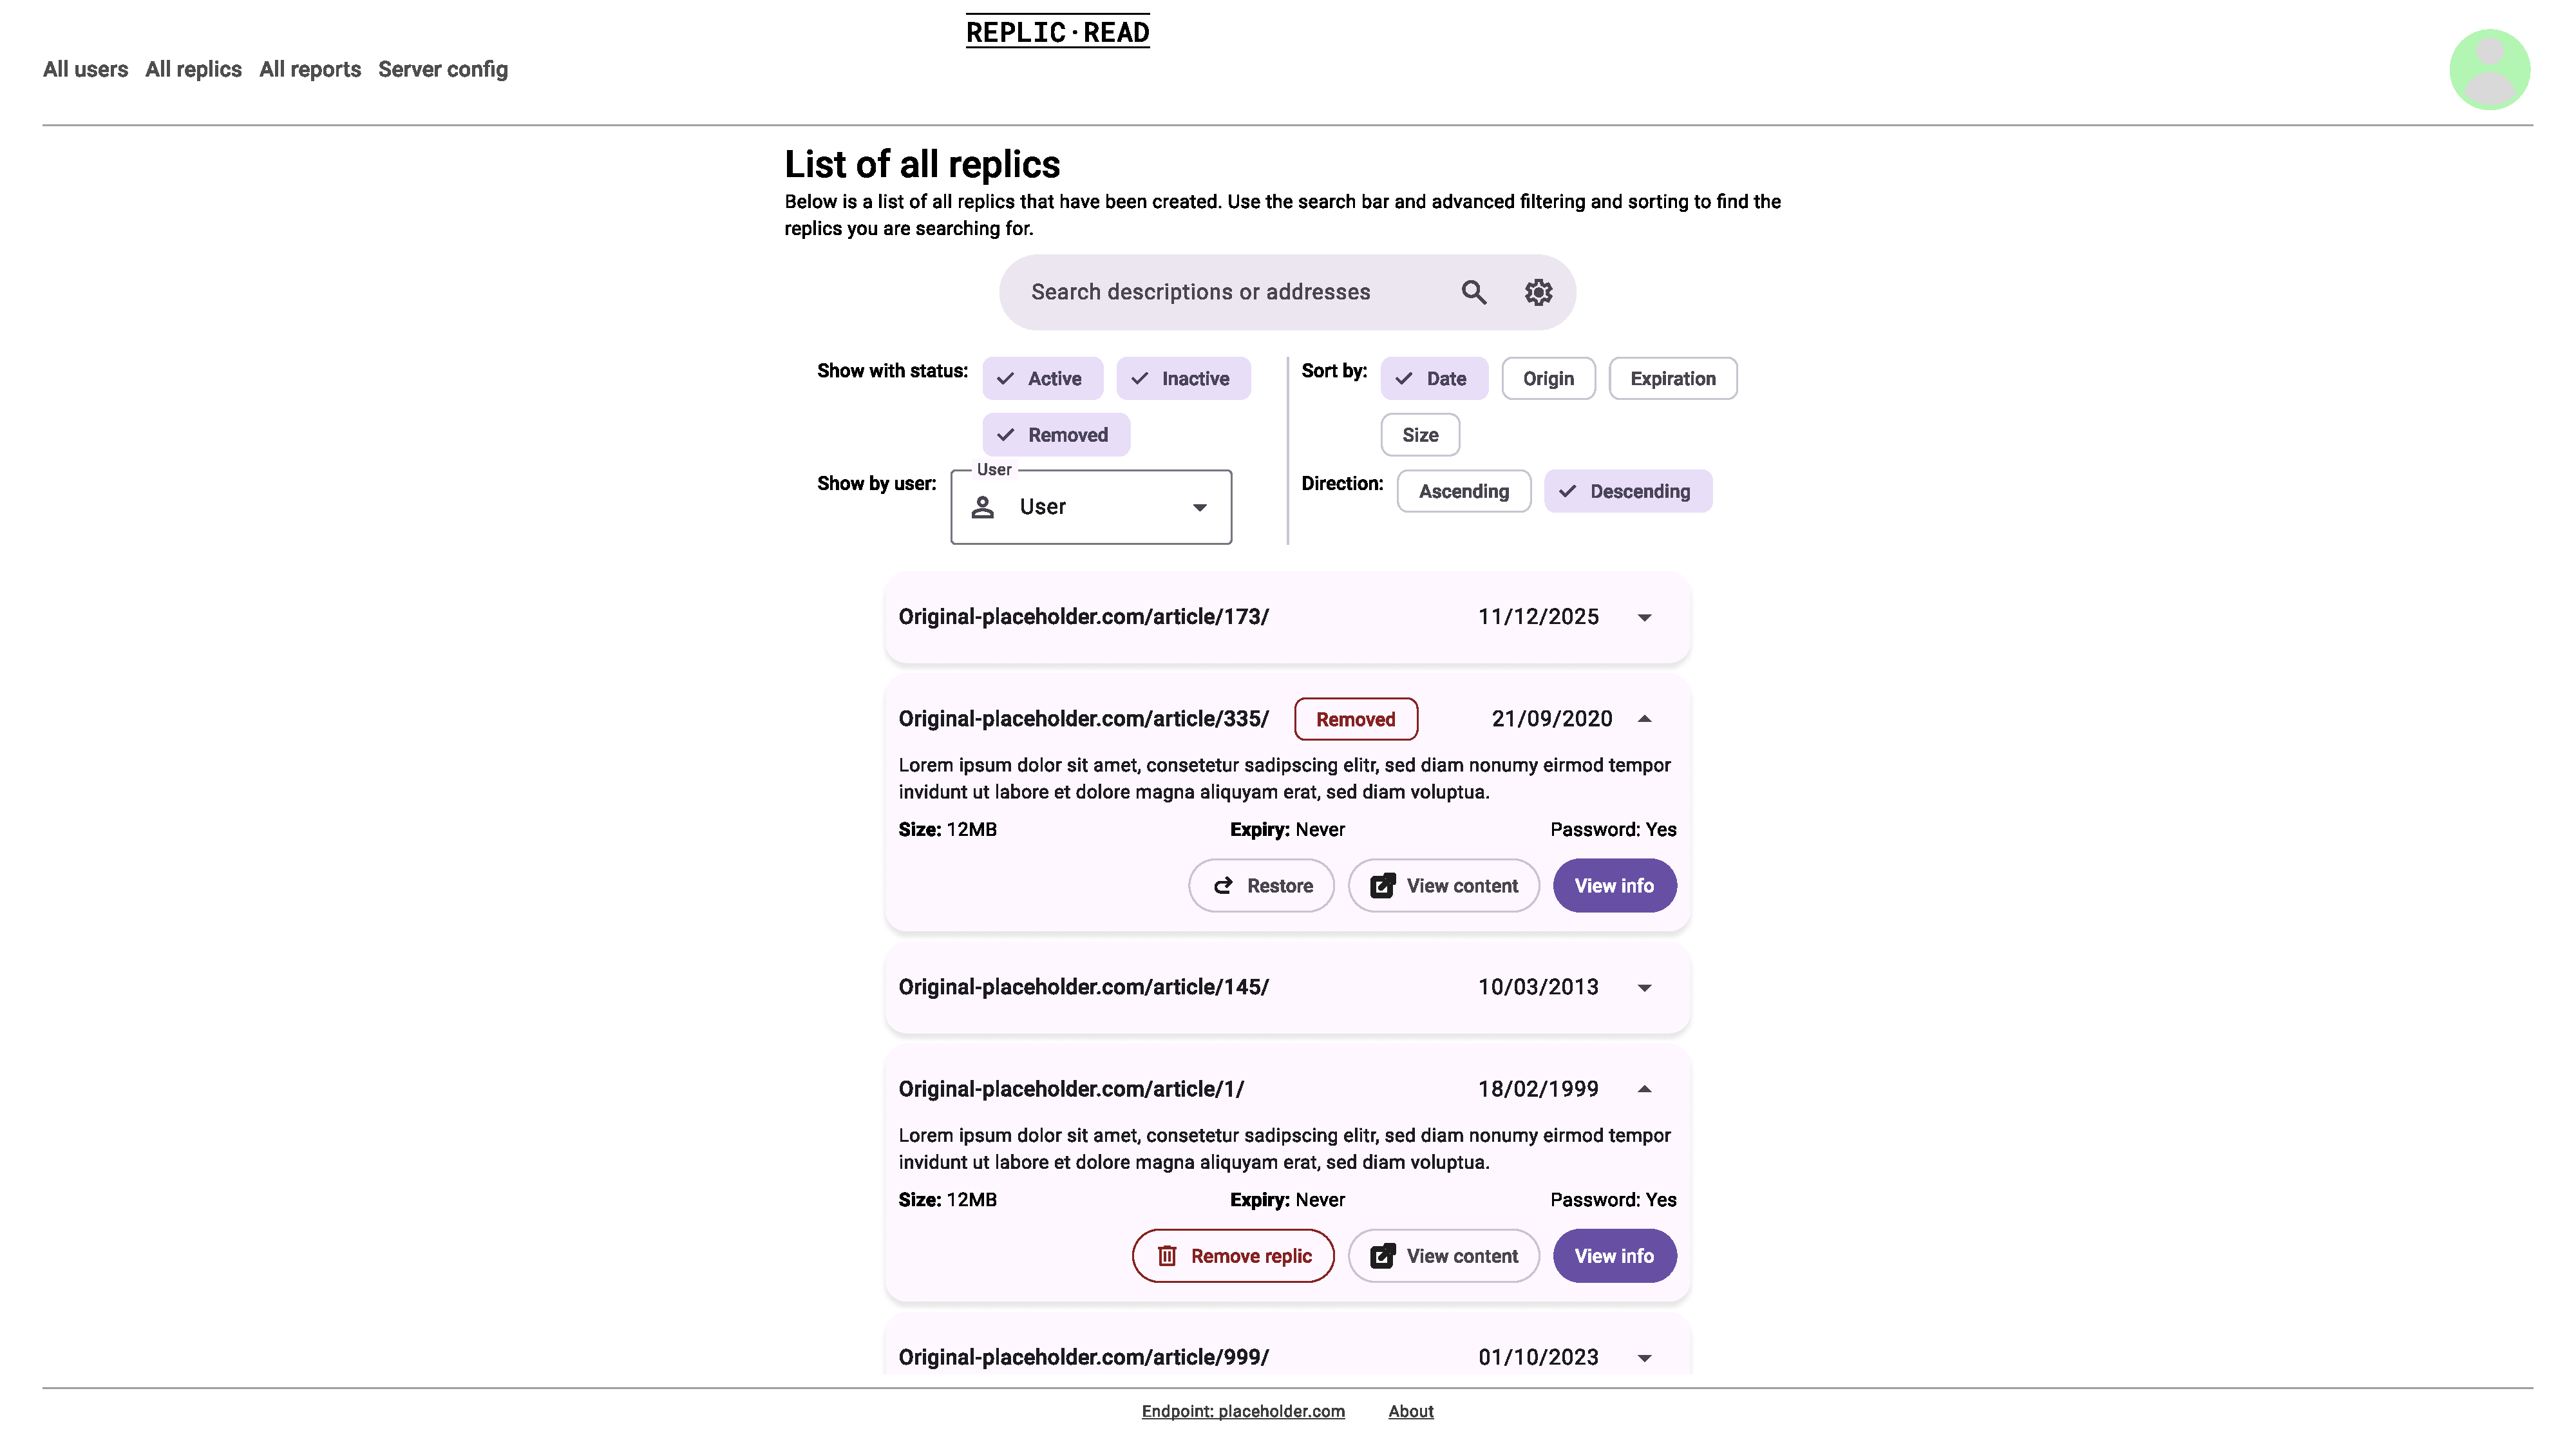
\includegraphics[width=12cm]{web-admin-replics-config}}

    \caption{Admin replics view with search config visible}
    \label{fig:web-admin-replics-config-view}
\end{figure}
\begin{figure}
    \centering
    \fbox{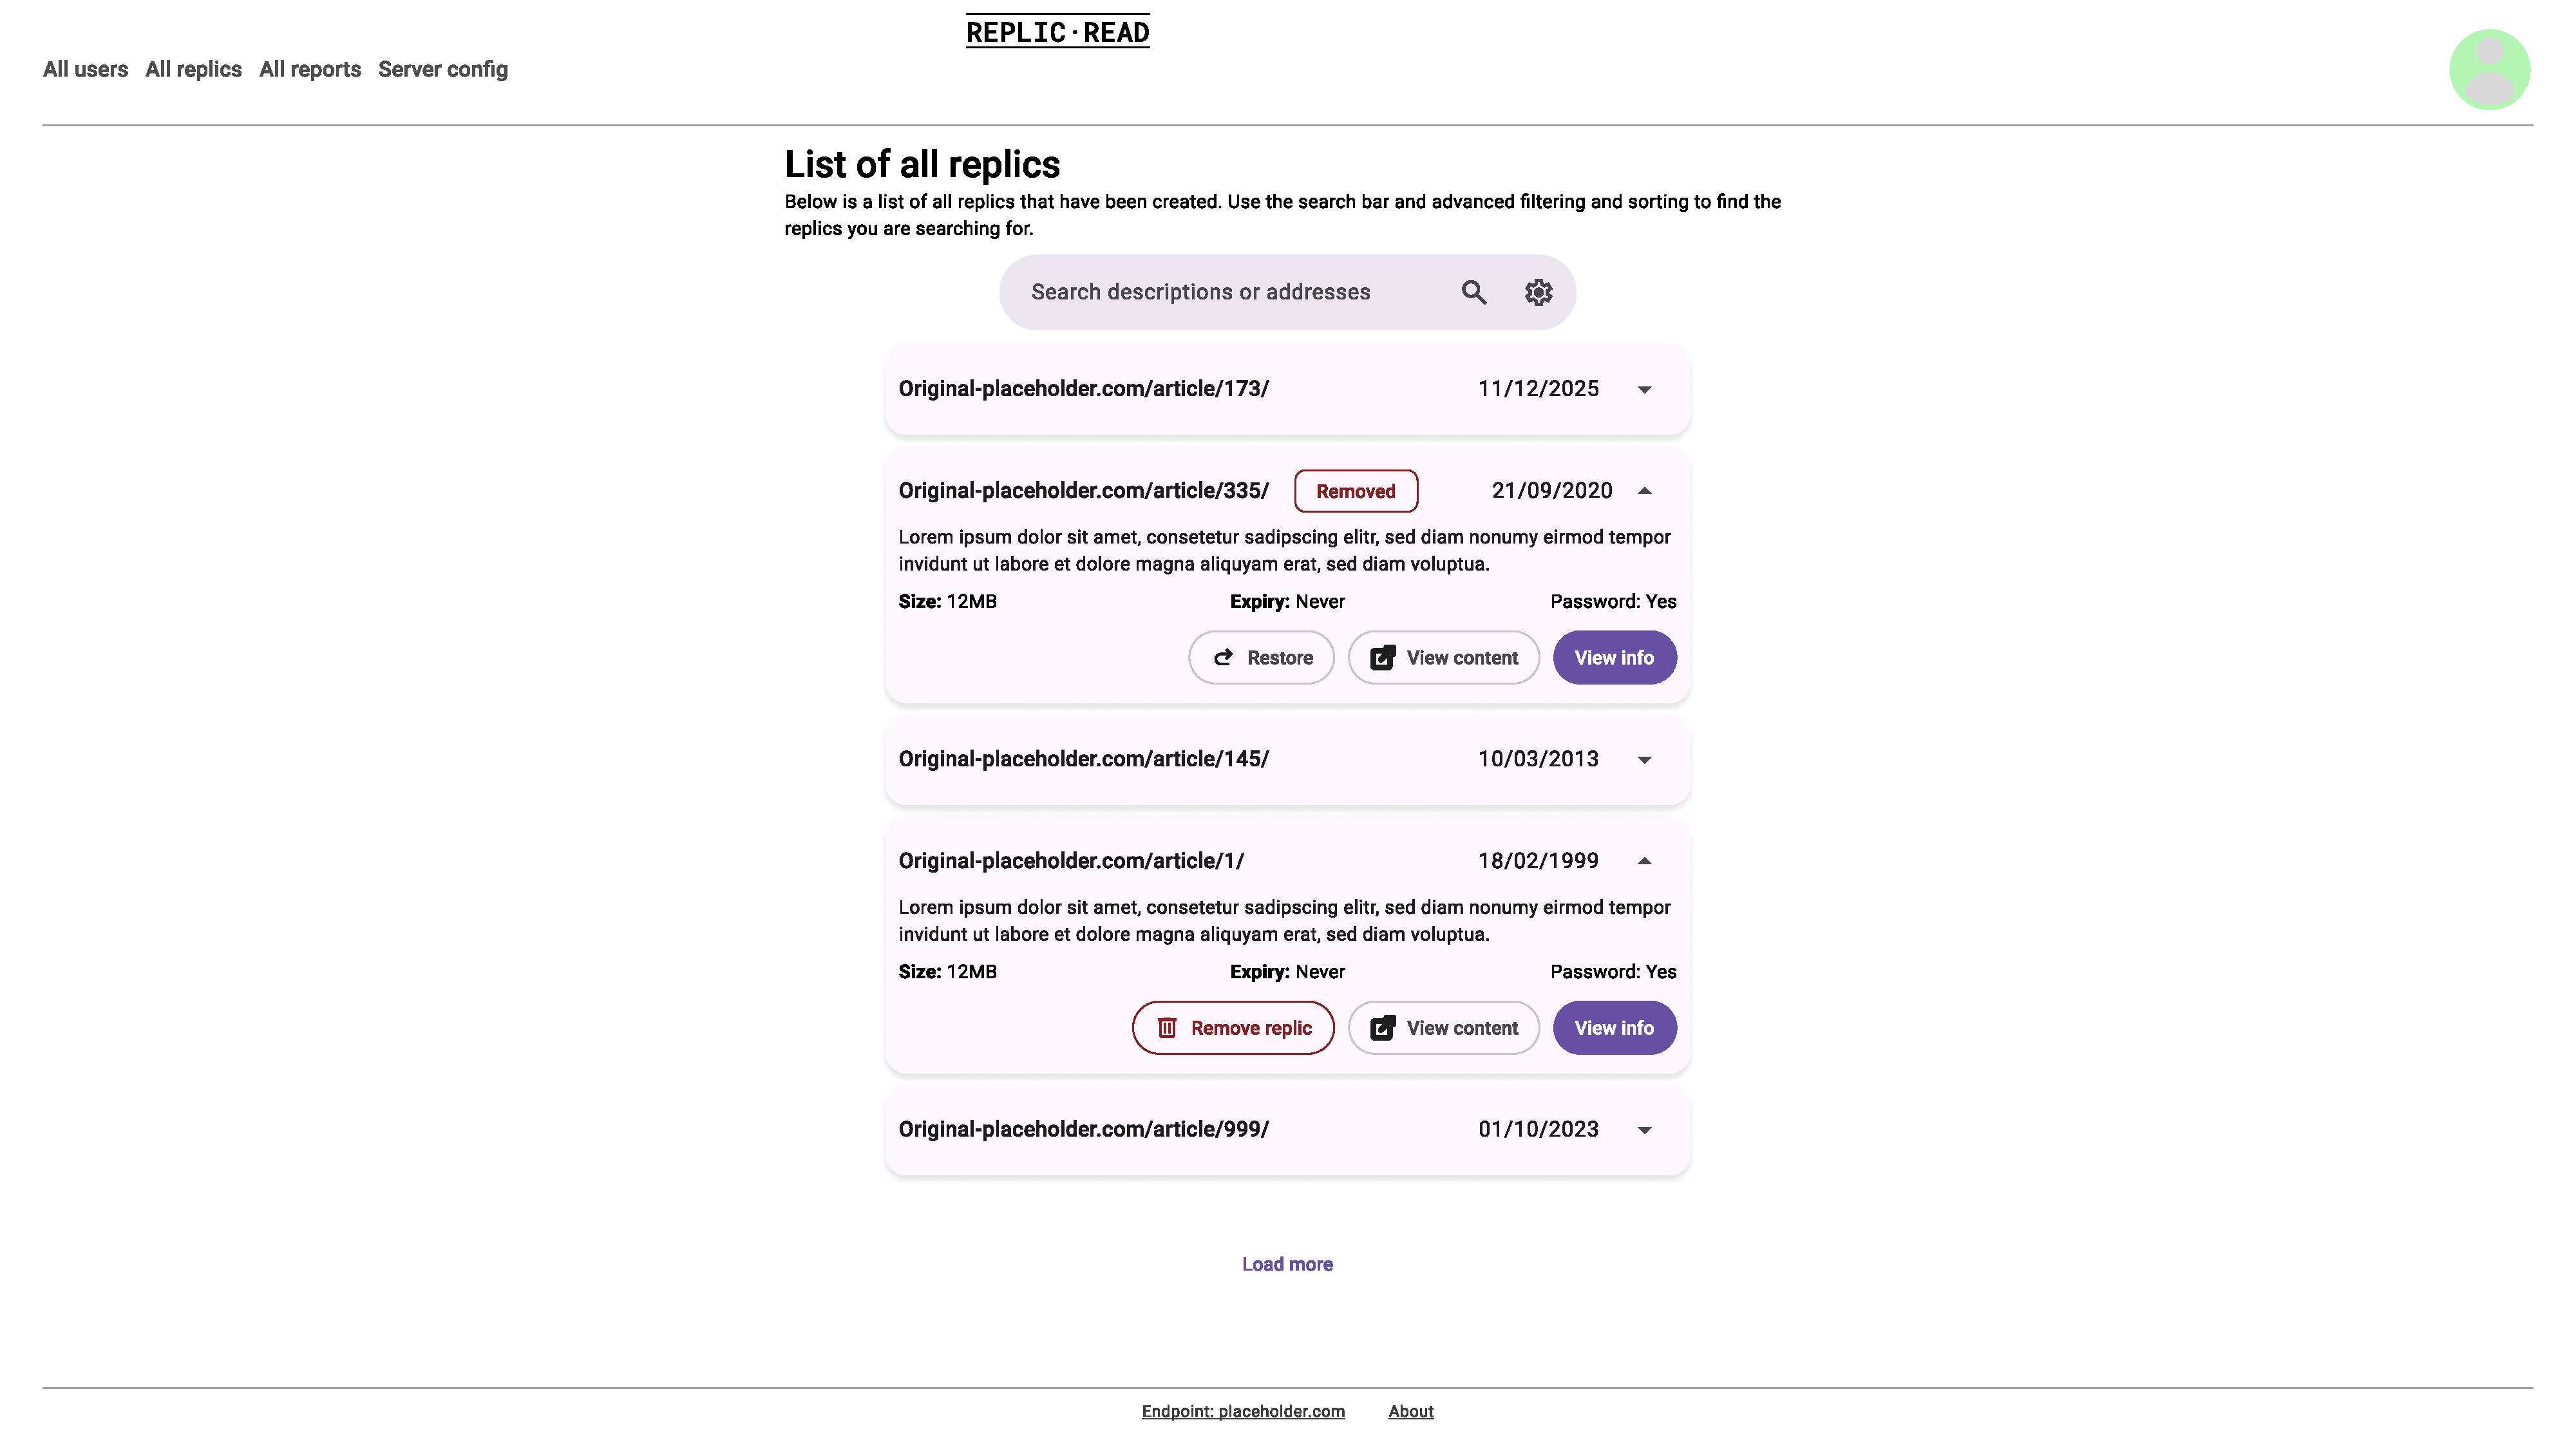
\includegraphics[width=12cm]{web-admin-replics-noconfig}}

    \caption{Admin replics view}
    \label{fig:web-admin-replics-noconfig-view}
\end{figure}

\subsubsection{Admin accounts view}
The admin accounts view allows the admin to view all accounts on the server.
Each account is represented by an item in a list that shows the username, profile color and email-address.
Each item has context actions that allow the admin to deactivate (\ref{subsubsec:deactivate-acc-admin}) or reactivate (\ref{subsubsec:reactivate-acc-admin}) an account, and to reset an account's password (\ref{subsubsec:reset-pass}).
The accounts can be searched using a search bar, and filtered/sorted by using the sorting config that can be expanded (\ref{fig:web-accounts-config-view}) or collapsed (\ref{fig:web-accounts-noconfig-view}).
\begin{figure}
    \centering
    \fbox{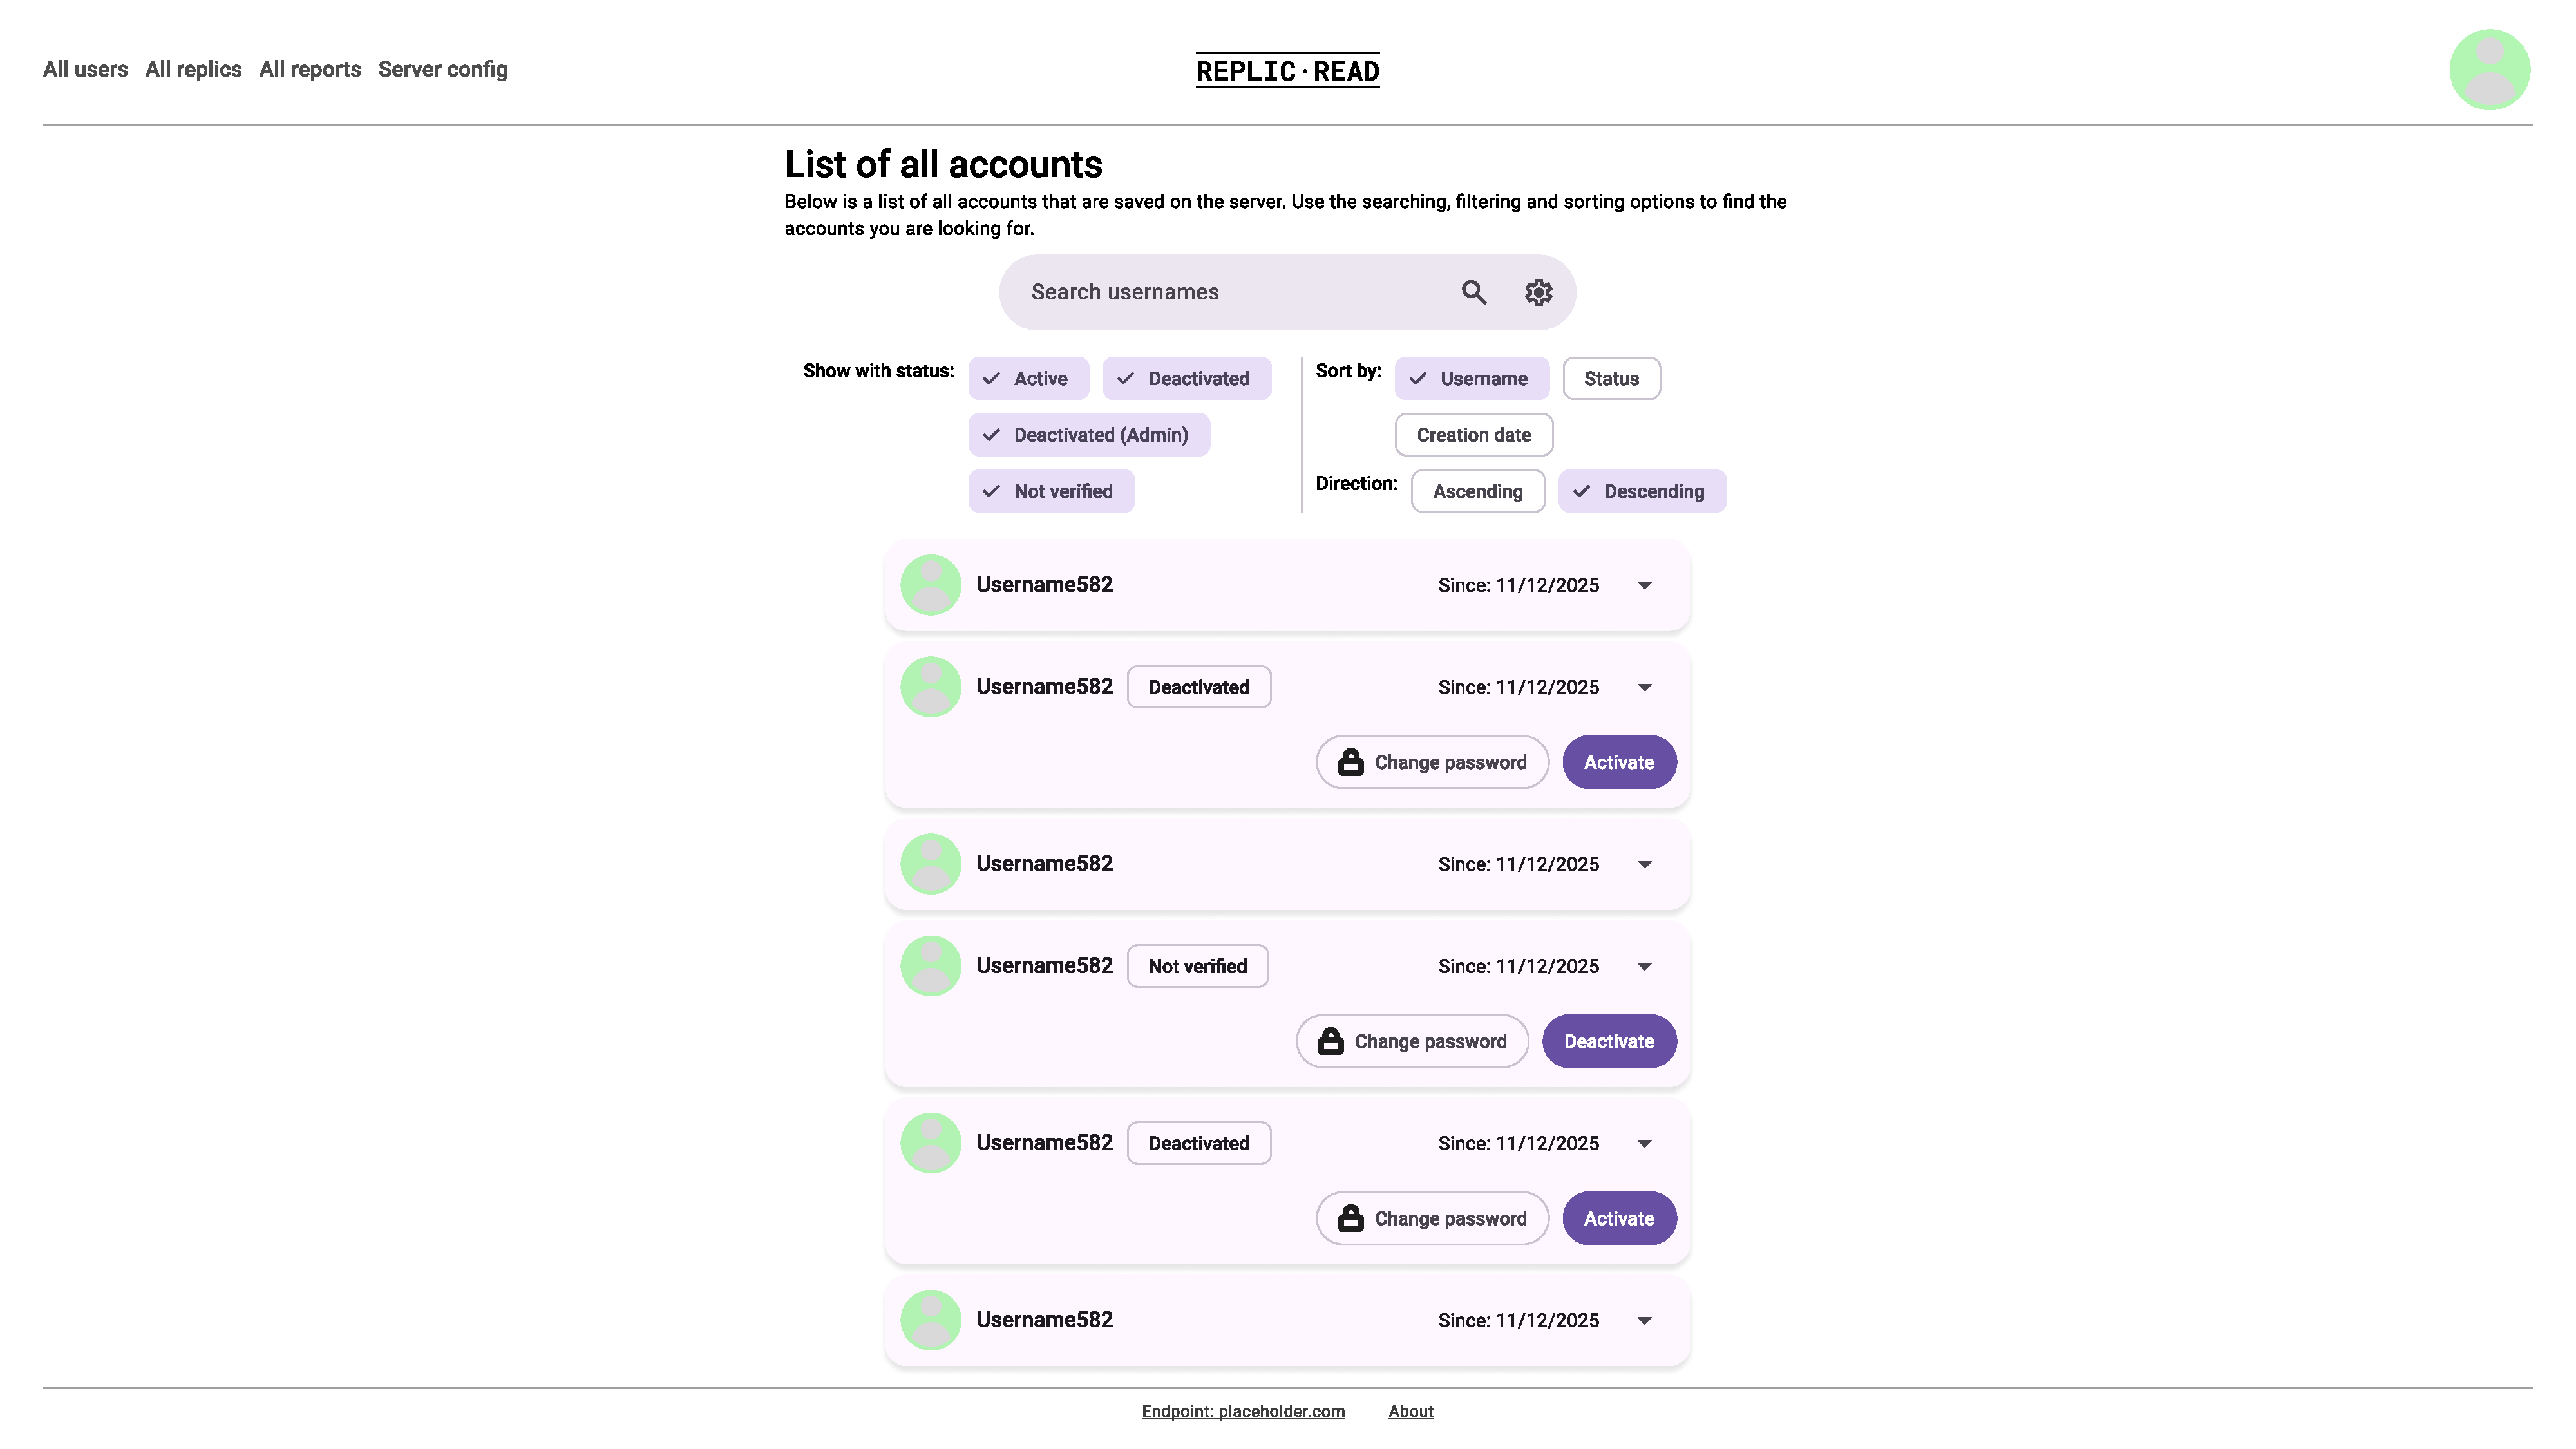
\includegraphics[width=12cm]{web-accounts-config}}

    \caption{Admin accounts view with search config visible}
    \label{fig:web-accounts-config-view}
\end{figure}
\begin{figure}
    \centering
    \fbox{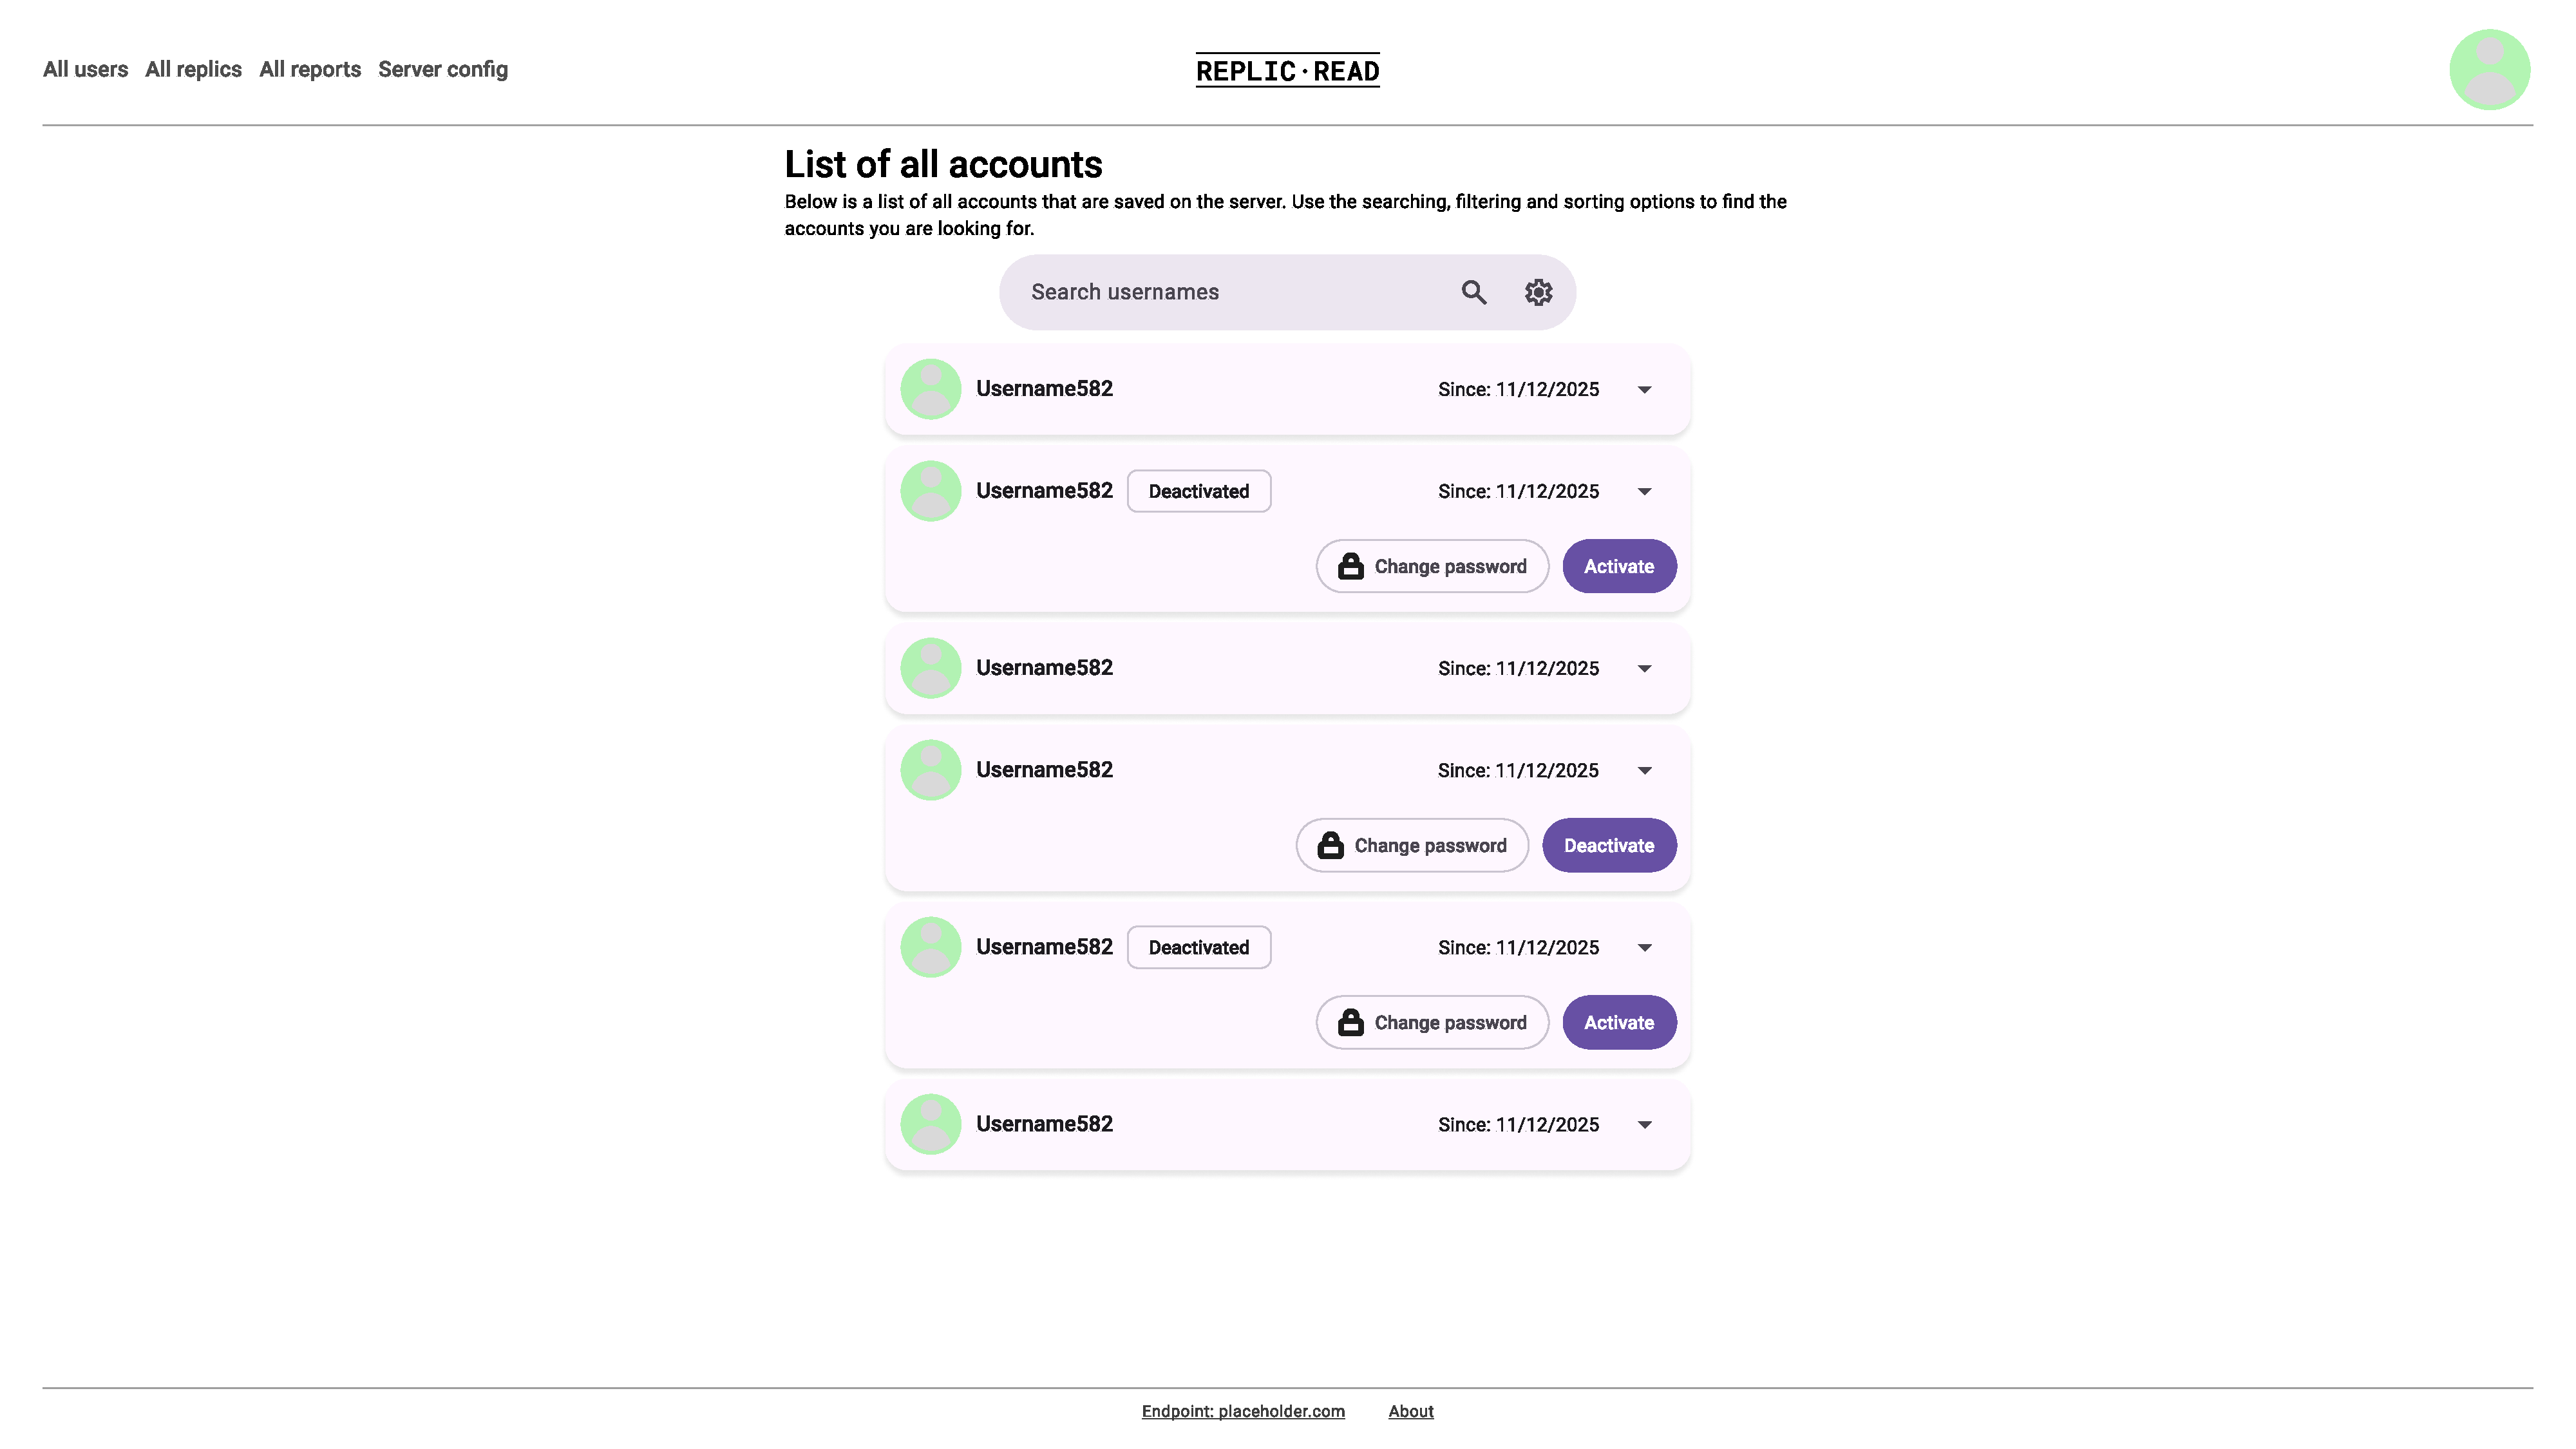
\includegraphics[width=12cm]{web-accounts-noconfig}}

    \caption{Admin accounts view}
    \label{fig:web-accounts-noconfig-view}
\end{figure}

\subsubsection{Admin reports view}
The admin reports view allows the admin to view all open reports that have been made (by users).
Each report is represented by an item in a list that shows the author, submission date and description.
Each item has context actions that allow the admin to review (\ref{subsubsec:review-report}) or close a report.
The reports can be searched using a search bar, and filtered/sorted by using the sorting config that can be expanded (\ref{fig:web-reports-config-view}) or collapsed (\ref{fig:web-reports-noconfig-view}).
\begin{figure}
    \centering
    \fbox{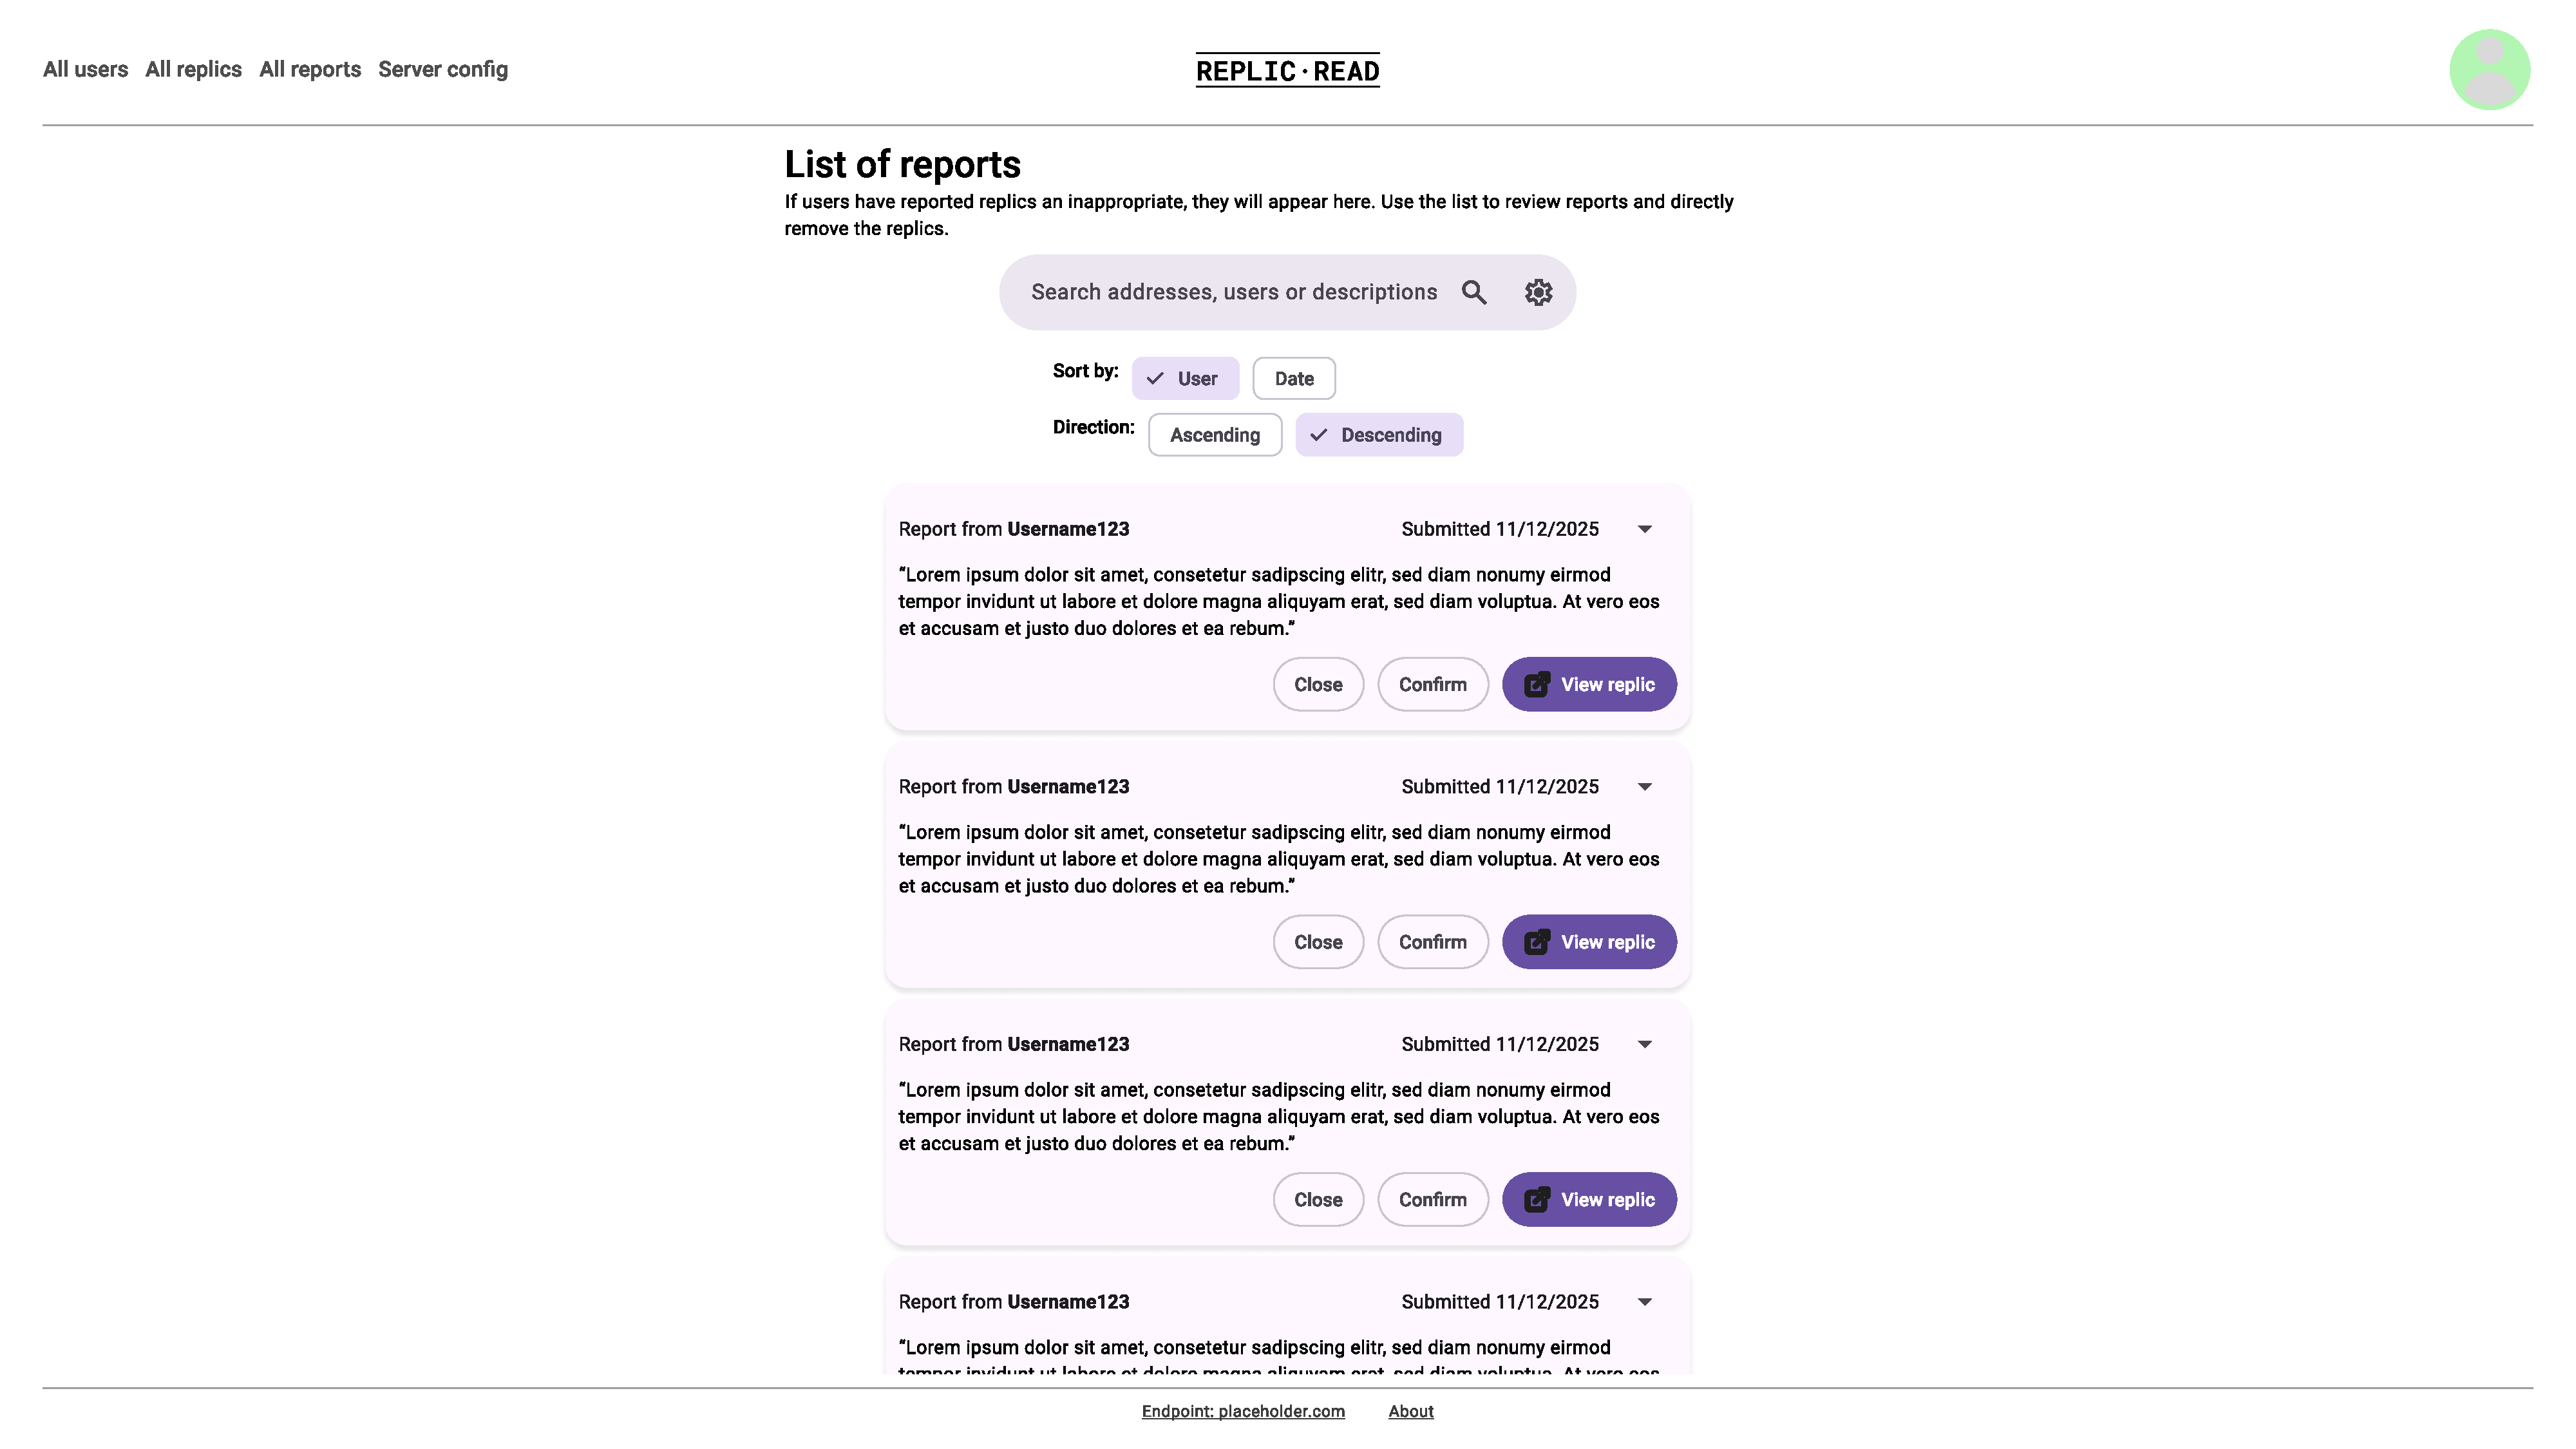
\includegraphics[width=12cm]{web-reports-config}}

    \caption{Admin reports view with search config visible}
    \label{fig:web-reports-config-view}
\end{figure}
\begin{figure}
    \centering
    \fbox{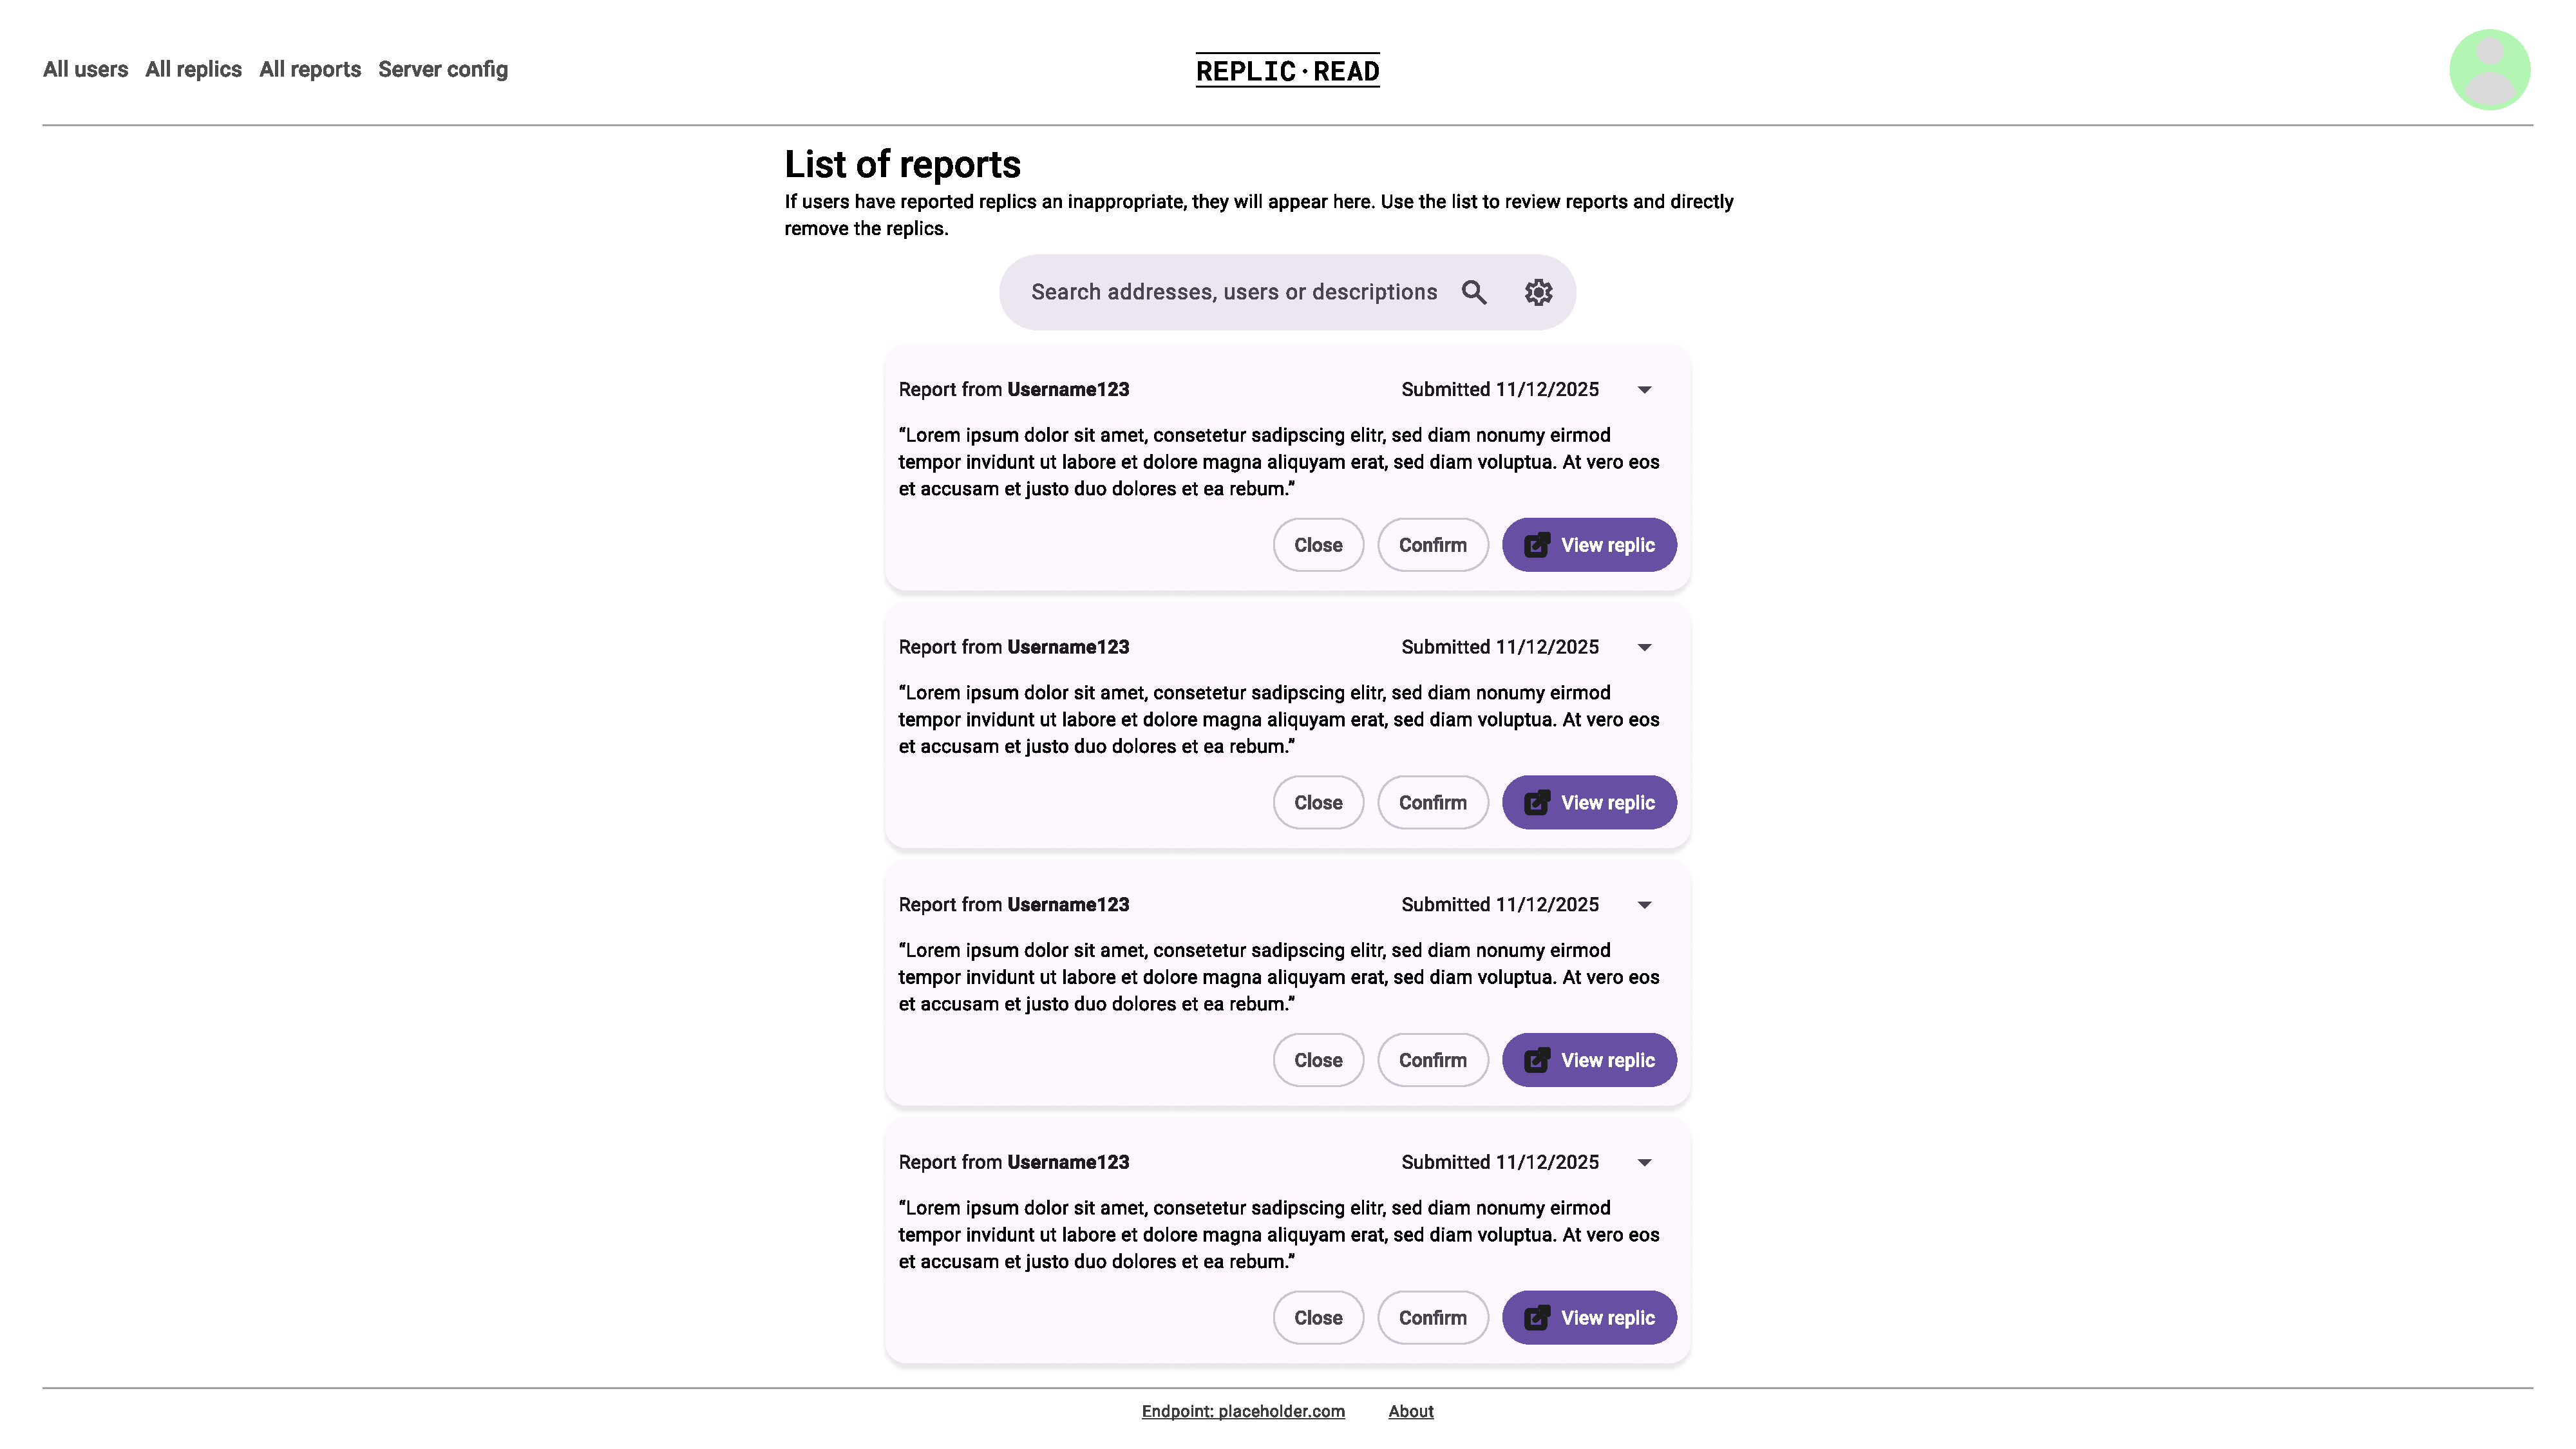
\includegraphics[width=12cm]{web-reports-noconfig}}

    \caption{Admin reports view}
    \label{fig:web-reports-noconfig-view}
\end{figure}

\subsubsection{Replic view}
The replic view (\ref{fig:web-replic-active-view}) shows information about a specific replic and allows the user to view the replic's content.
If the replic is not accessible anymore, it is shown to the user (\ref{fig:web-replic-inactive-view}).
\begin{figure}
    \centering
    \fbox{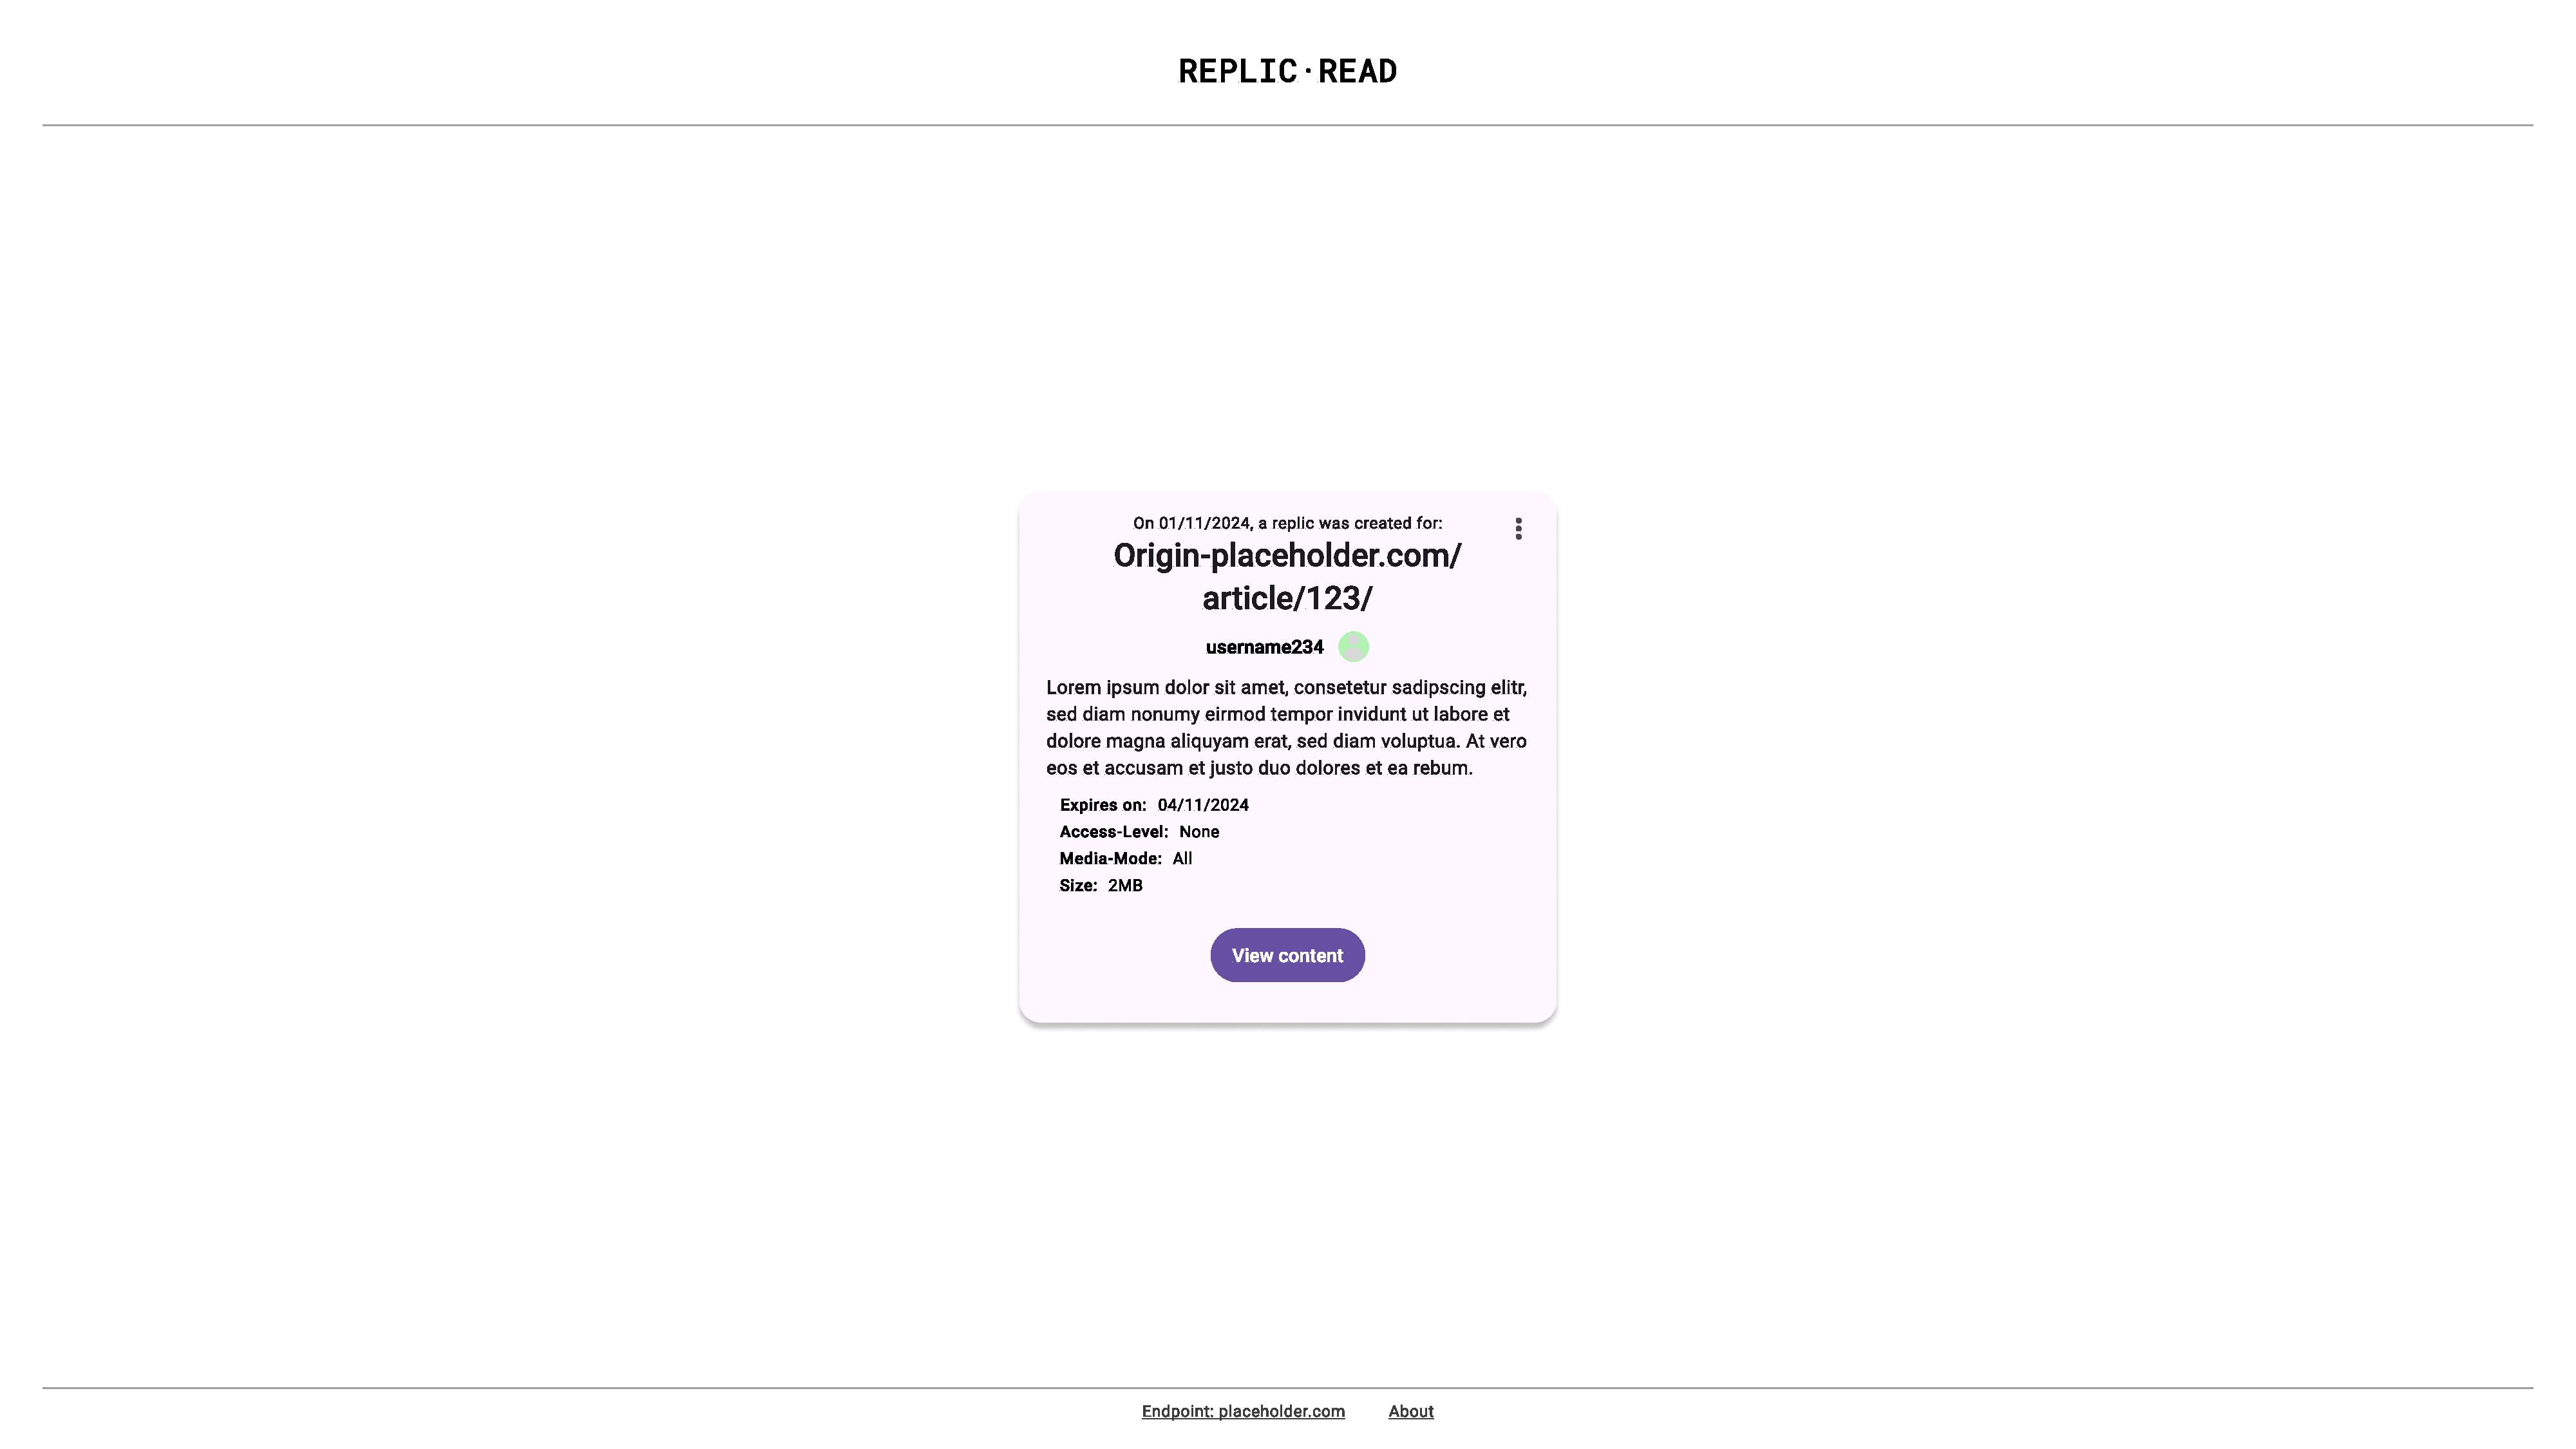
\includegraphics[width=12cm]{web-replic-active}}

    \caption{Active replic view}
    \label{fig:web-replic-active-view}
\end{figure}
\begin{figure}
    \centering
    \fbox{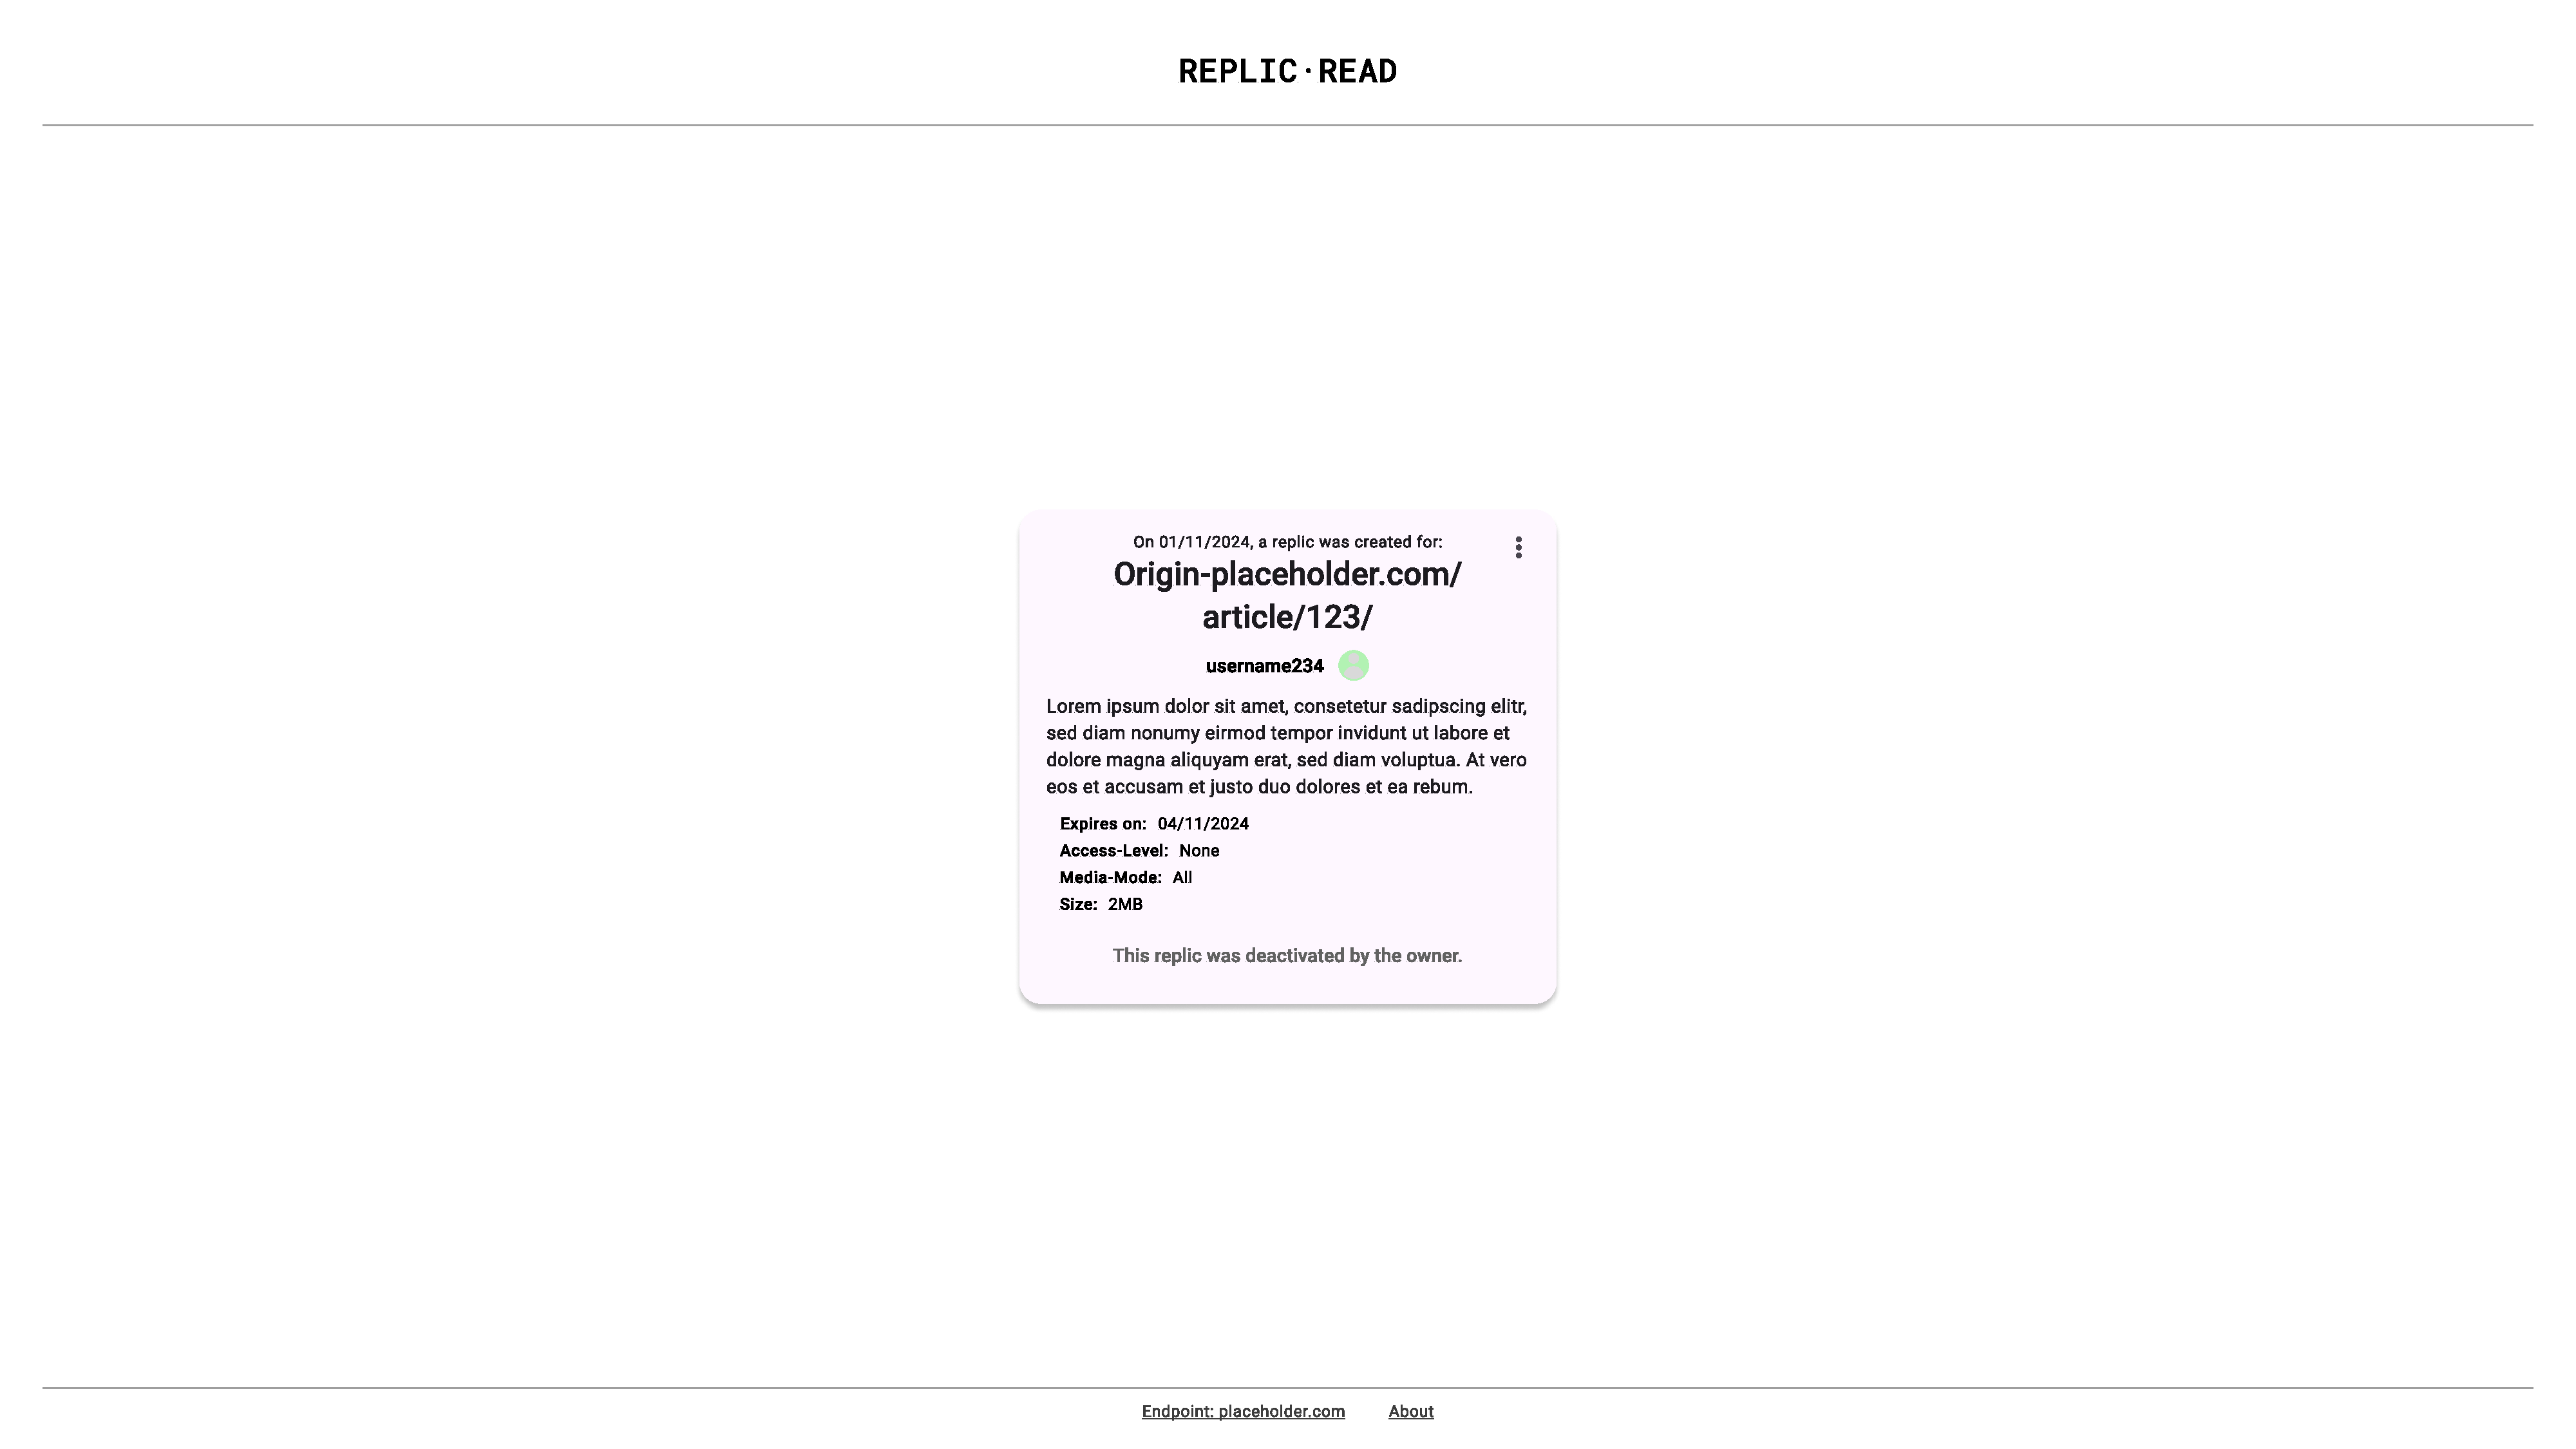
\includegraphics[width=12cm]{web-replic-inactive}}

    \caption{Inactive replic view}
    \label{fig:web-replic-inactive-view}
\end{figure}

\subsubsection{Email-Verification view}
The email-verification view is shown to the user when an email-erification link, that was sent via email, was used.
It either shows a message indicating the success (\ref{fig:web-email-verification-error}) or the failure (\ref{fig:web-email-verification-success}) of the verification process.

\begin{figure}
    \centering
    \fbox{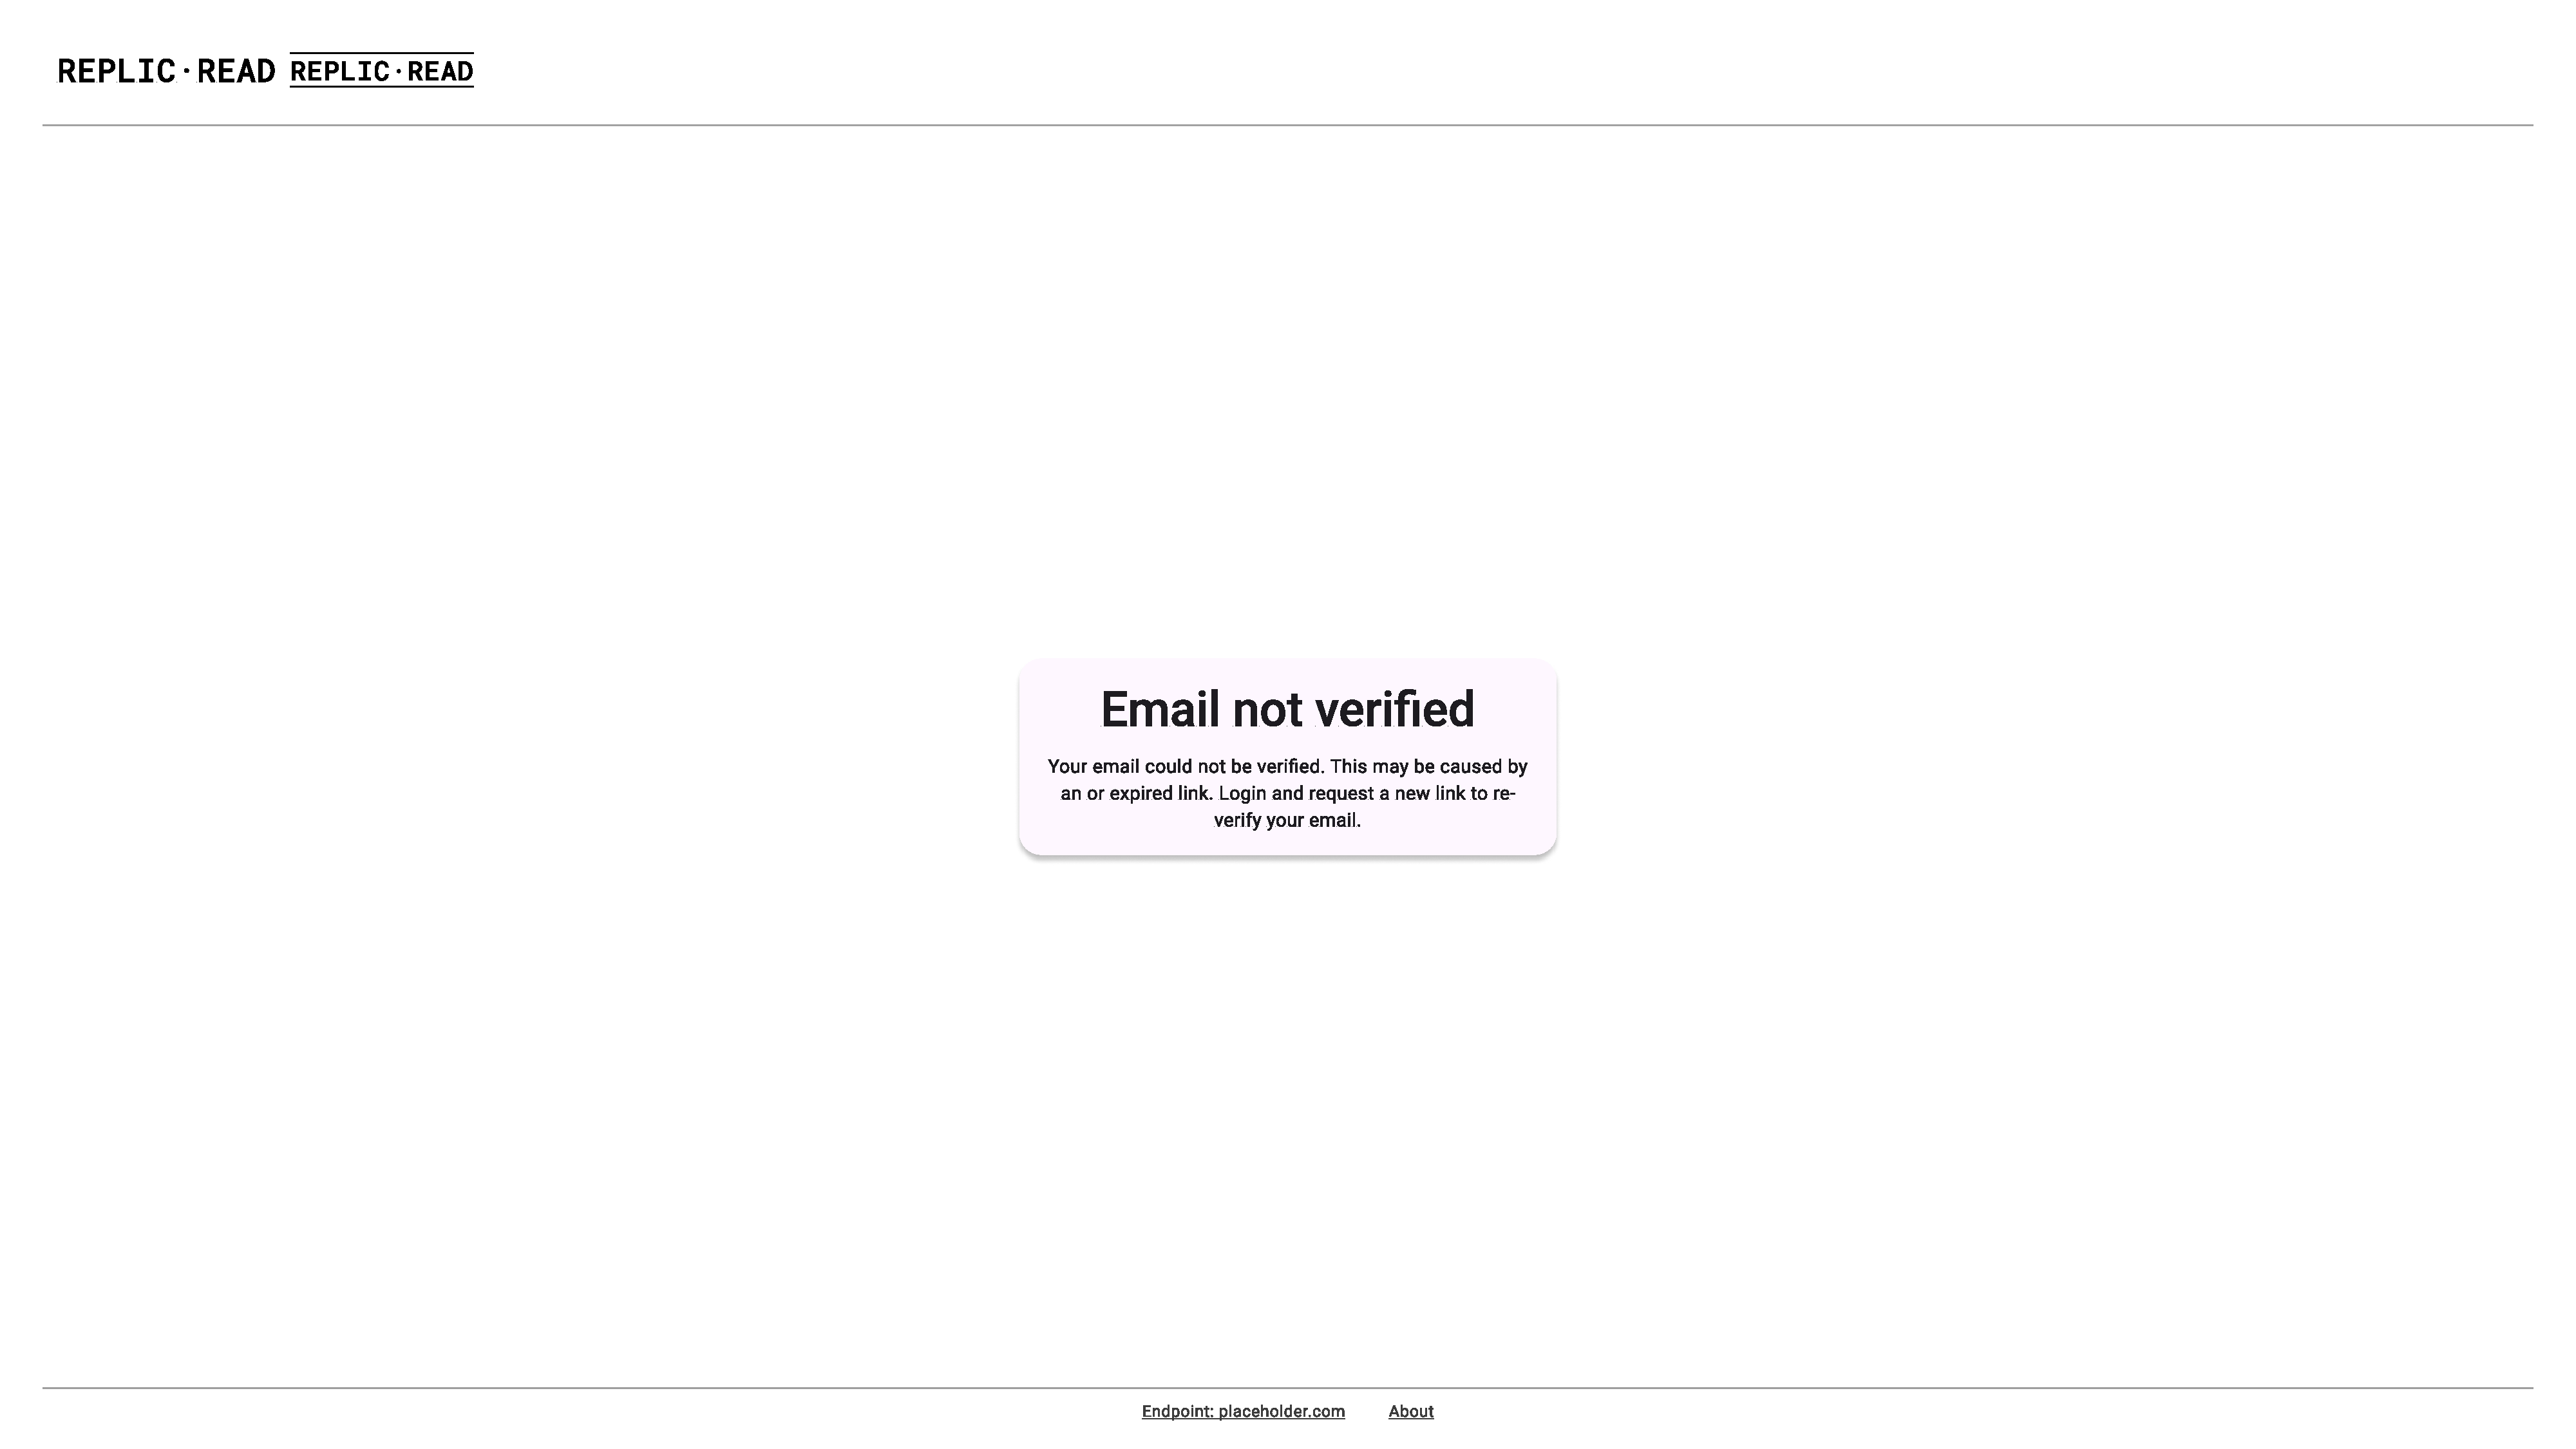
\includegraphics[width=12cm]{web-email-verification-error}}

    \caption{Email-verification view with failure status}
    \label{fig:web-email-verification-error}
\end{figure}
\begin{figure}
    \centering

    \fbox{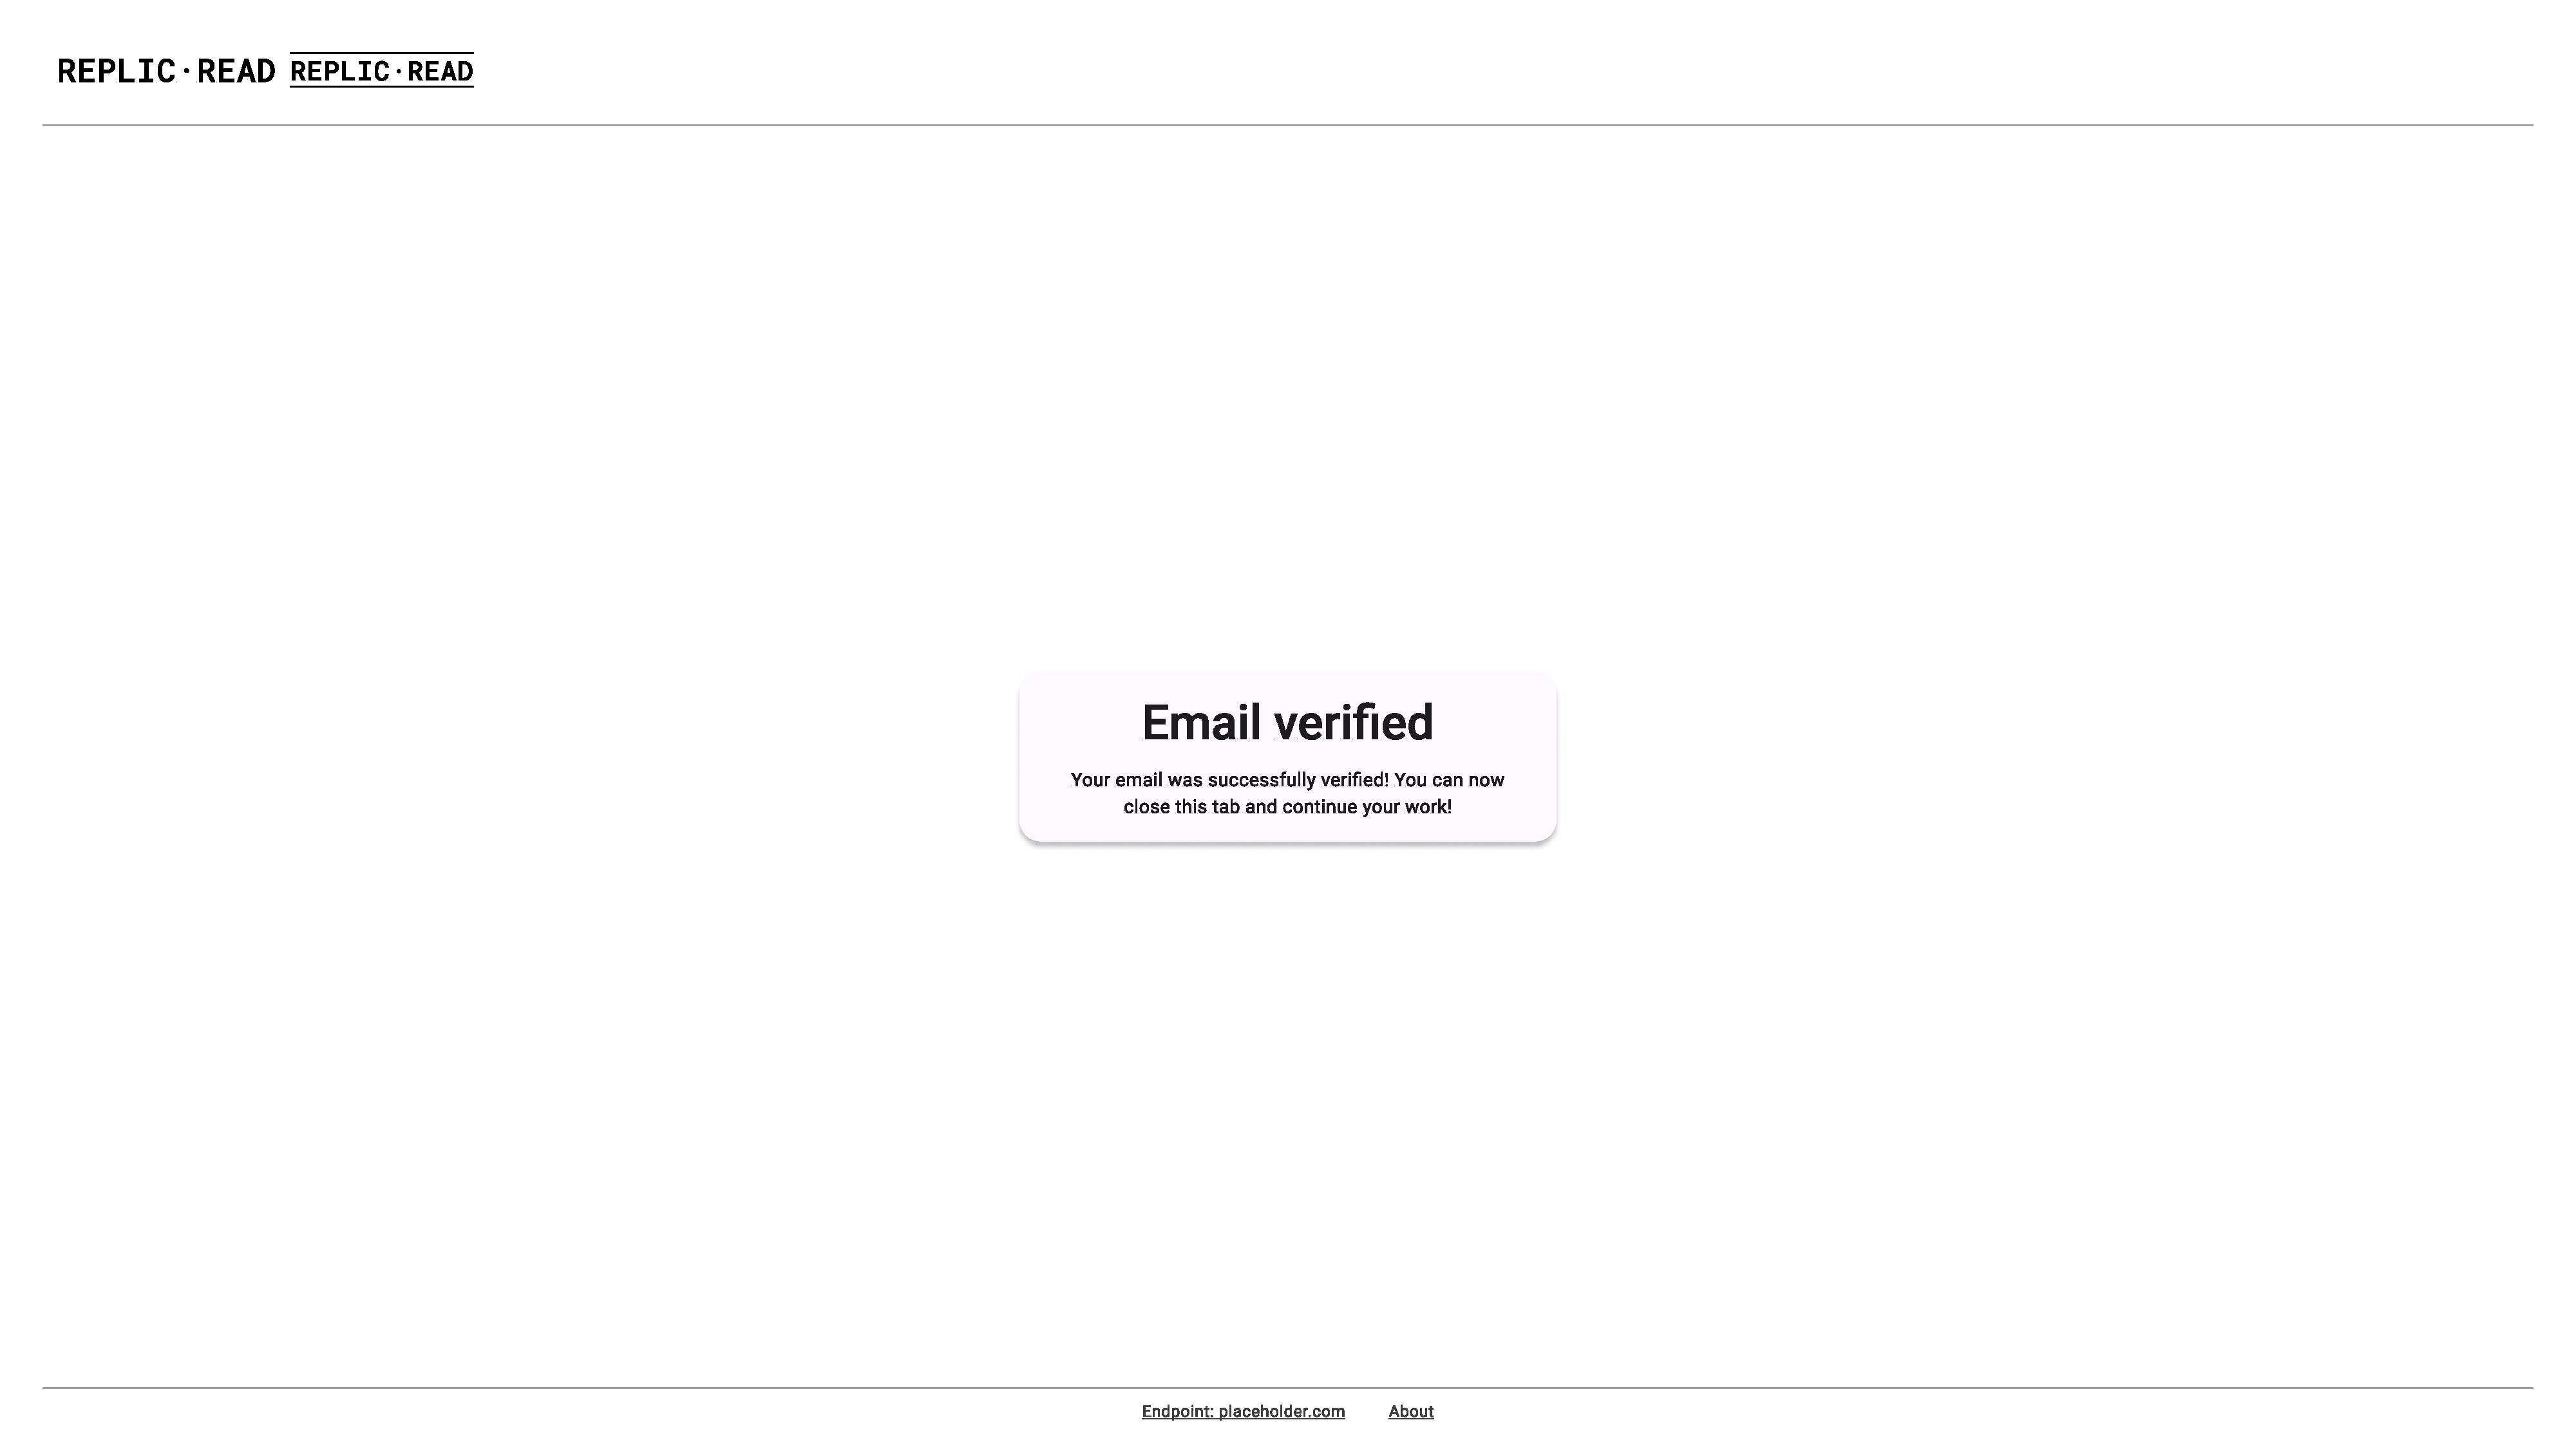
\includegraphics[width=12cm]{web-email-verification-success}}

    \caption{Email-verification view with success status}
    \label{fig:web-email-verification-success}
\end{figure}

\subsubsection{Email-not-verified view}
The email-not-verified view (\ref{fig:web-email-not-verified}) is shown to the user when an operation is attempted that requires the email to be verified.

\begin{figure}
    \centering
    \fbox{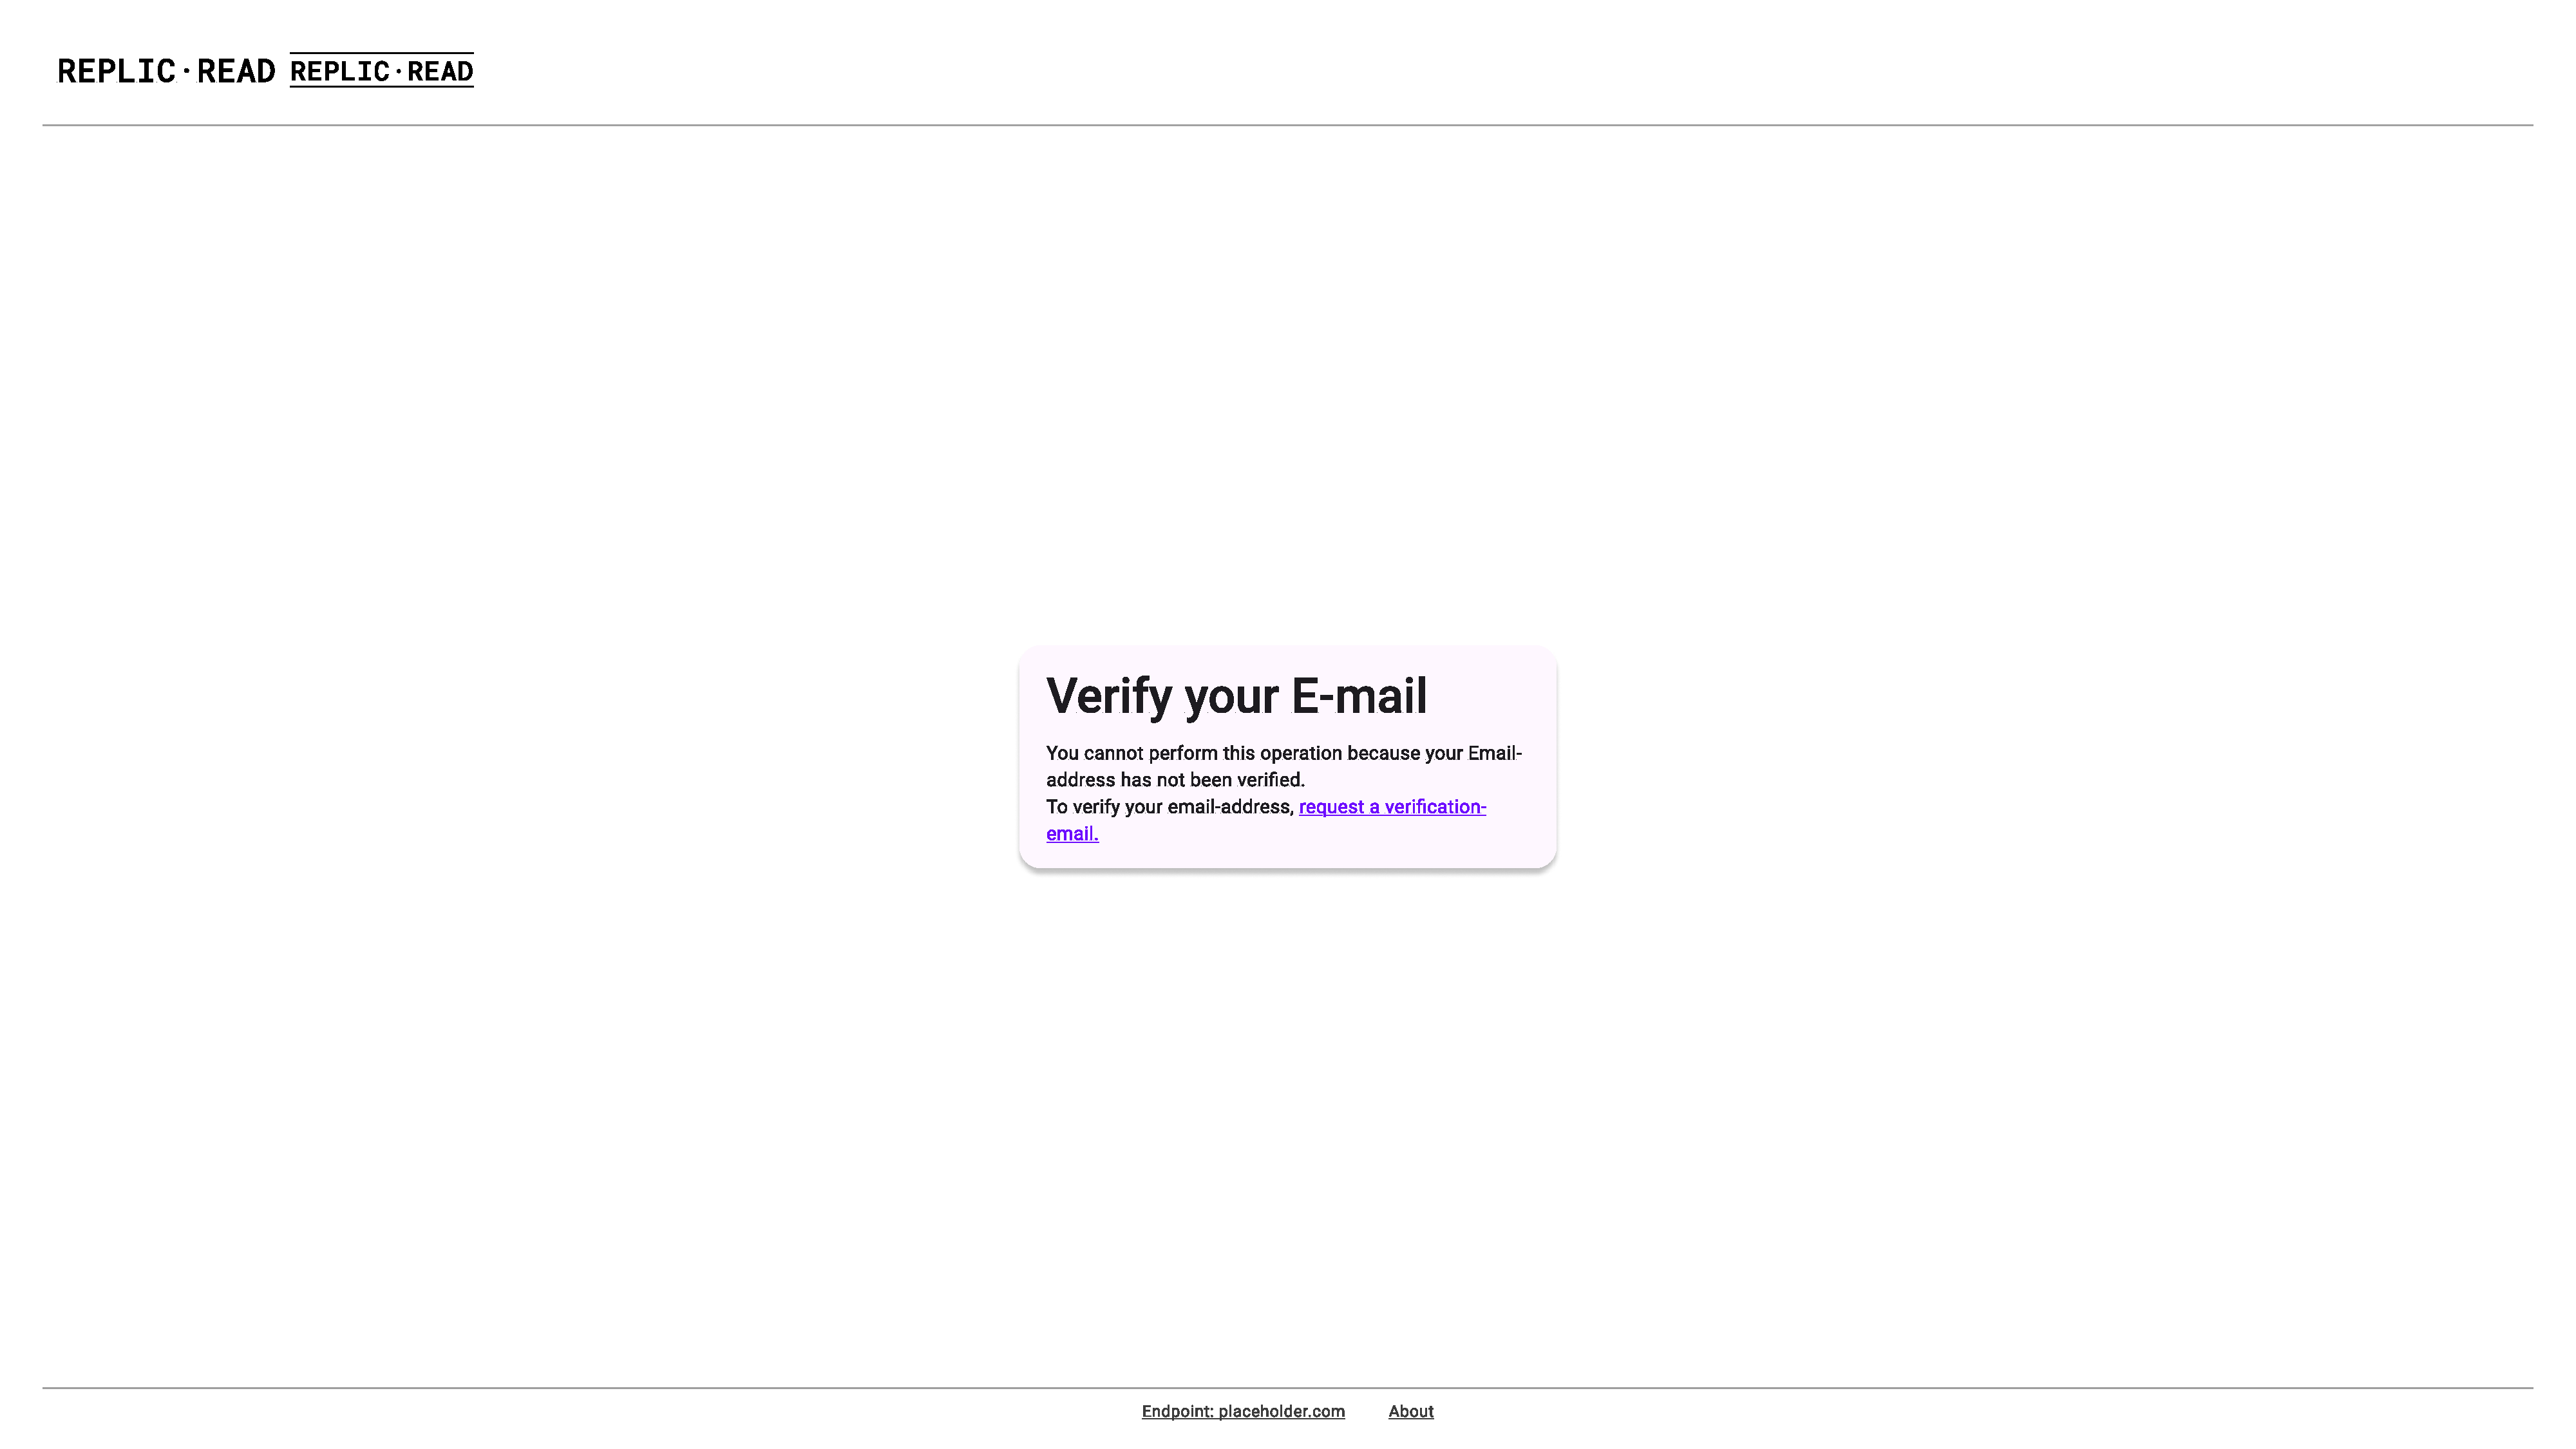
\includegraphics[width=12cm]{web-email-not-verified}}

    \caption{Email-not-verified view}
    \label{fig:web-email-not-verified}
\end{figure}